%%% The main file. It contains definitions of basic parameters and includes all other parts.

\documentclass[a4paper,oneside]{memoir}
\usepackage[english]{babel}
\usepackage[T1]{fontenc}
\usepackage[utf8]{inputenc}
\usepackage{wallpaper}
\usepackage{palatino}
\usepackage[toc,page]{appendix}



% \openright makes the following text appear on a right-hand page
\let\openright=\clearpage

%% Settings for two-sided (duplex) printing
% \documentclass[12pt,a4paper,twoside,openright]{report}
% \setlength\textwidth{145mm}
% \setlength\textheight{247mm}
% \setlength\oddsidemargin{14.2mm}
% \setlength\evensidemargin{0mm}
% \setlength\topmargin{0mm}
% \setlength\headsep{0mm}
% \setlength\headheight{0mm}
% \let\openright=\cleardoublepage

%% Generate PDF/A-2u
\usepackage[a-2u]{pdfx}

%% Character encoding: usually latin2, cp1250 or utf8:
\usepackage[utf8]{inputenc}

%% Prefer Latin Modern fonts
\usepackage{lmodern}

%% Further useful packages (included in most LaTeX distributions)
\usepackage{amsmath}        % extensions for typesetting of math
\usepackage{mathtools}
\usepackage{amsfonts}       % math fonts
\usepackage{amsthm}         % theorems, definitions, etc.
\usepackage{bbding}         % various symbols (squares, asterisks, scissors, ...)
\usepackage{bm}             % boldface symbols (\bm)
\usepackage{graphicx}       % embedding of pictures
\usepackage{fancyvrb}       % improved verbatim environment
\usepackage{natbib}         % citation style AUTHOR (YEAR), or AUTHOR [NUMBER]
\usepackage[nottoc]{tocbibind} % makes sure that bibliography and the lists
			    % of figures/tables are included in the table
			    % of contents
\usepackage{dcolumn}        % improved alignment of table columns
\usepackage{booktabs}       % improved horizontal lines in tables
\usepackage{paralist}       % improved enumerate and itemize
\usepackage[usenames]{xcolor}  % typesetting in color
\usepackage{caption}
\usepackage{subcaption}

\setcounter{tocdepth}{4}
\setcounter{secnumdepth}{4}

%%% Basic information on the thesis

\def\ThesisType{Master Thesis}

%\def\ThesisTitle{Unsupervised Anomaly Detection on Log Data}

%\def\ThesisTitle{Unsupervised Anomaly Detection on Motorola Solution's Unstructured Log Data}

\def\ThesisTitle{Log-Based Unsupervised Anomaly Detection in Mission Critical Radio System}

%\def\ThesisTitle{Anomaly Detection on Log Data Using Unsupervised Machine Learning Techniques}

%\def\ThesisTitle{Unsupervised Anomaly Detection in Unstructured Logs}


\def\ThesisSubtitle{}

\def\SupervisorName{Tijs Slaats}

\def\SupervisorMail{slaats@di.ku.dk}

\def\SupervisorCompanyName{Lucian Tirca}

\def\SupervisorCompanyMail{lucian.tirca@motorolasolutions.com}

\def\StudentFirstName{Gabriela Dvořáková}

\def\StudentFirstMail{kzh186@alumni.ku.dk}

\def\StudentSecondName{Denis Drobný}

\def\StudentSecondMail{htp440@alumni.ku.dk}

% An optional dedication: you can thank whomever you wish (your supervisor,
% consultant, a person who lent the software, etc.)
\def\Acknowledgements{
First and foremost, we would like to thank Motorola Solutions Denmark for giving us the wonderful opportunity to intern there and give us a glimpse into the development of such a complex software product. We are very grateful for their efforts in making us feel comfortable in their work environment throughout the thesis writing process. It was a great experience. 

We would like to thank our university supervisor Tijs Slaats for his continuous guidance, insightful comments and time spent during our meetings and reading our thesis. 

Also, our big thanks go to Lucian Tirca, our company supervisor, who threw around great ideas and always helped us with our struggles. His endless patience and positivity made the whole research a pleasure. 

We would also like to thank the members of the SmartConnect team for every bit of advice. We also appreciated the fruitful discussions with Maarten Faddegon and Jakub Slupecki at Motorola and their reviews throughout the process.

Not to forget, we send hugs to our very informal supervisors Miguel Angel Tovar(ish) and Laura Victoria Florez, who helped us complete the mission.

%First and foremost, we would like to thank our supervisors. 
%Tijs Slaats, our supervisor at the University of Copenhagen, who gave us valuable advice, feedback and assessments.
%Our big thanks also go to Lucian Tirca, the supervisor for Motorola Solutions, who was always very patient, positive and full of ideas.

%We would also like to thank Motorola Solutions Denmark for giving us the opportunity to become part of them for the period of writing the thesis, which allowed us to conduct our research on a very interesting software product. 
%We would like to thank the members of the SmartConnect team for every bit of advice.\\ 
%We also appreciated the fruitful discussions with Maarten Faddegon and Jakub Slupecki from Motorola as well as their reviews throughout the process.

%Not to forget, we send hugs to our very informal supervisors Miguel Angel Tovar and Laura Victoria Florez, who bore with us all the way.
}

% Abstract (recommended length around 80-200 words; this is not a copy of your thesis assignment!)
 
\def\Abstract{
In software systems, logging is traditionally introduced to record information about the execution of a program. Typically, logs are analyzed by humans after an obvious error occurs or is reported by an end user. 
However, as software grows, it is no longer possible to monitor application behavior and troubleshoot errors with the naked eye. 
Machine learning based anomaly detection can overcome these problems and eventually provide a tool to detect bugs at an early stage while they are still relatively harmless.
In our thesis, we analyze time series of log data produced by Motorola Solution's SmartConnect. We aim to prove that it is possible to detect anomalies in a log dataset produced by a real-world system consisting of two main actors - the infrastructure and the push-to-talk radios connected to SmartConnect. We propose an anomaly detection architecture that consists of collecting data from the system, applying log parsing with Drain3, extracting event count features, and feeding the extracted fixed-size time window form into various machine learning models. We use four anomaly detection techniques: Isolation Forest, PCA, Invariants Mining and Log Clustering.
Since this is a highly confidential domain, we had to find an efficient way to train machine learning models based solely on datasets generated in a test phase, which may be different from the datasets generated in the production environment. 
Two of the four algorithms, PCA and Log Clustering, achieved perfect accuracy on the test dataset in distinguishing between normal and anomalous behavior. To evaluate the models on the unknown dataset, we asked the experts from the SmartConnect team to evaluate the predictions. They confirmed that the PCA model was able to detect another anomaly that was not known before the experiment. However, due to the complexity and the large amount of logs they were given to study, they could not tell whether the models had correctly classified non-anomalous samples. Finally, we found that our models monitoring the system could also be used to gain insight into the code coverage of the system tests.
}

\def\RQFirst{Can anomaly detection be applied on the log data that are at the moment produced by Motorola Solutions SmartConnect
system?}

% turn into an overall goal

\def\RQSecond{Does a weighted event vector representation of raw log messages logged by Motorola Solution’s SmartConnect production system provide sufficient information for spotting anomalous outliers in the data?}

% fix the text inbetween, we dont need to be able to proof it 

\def\RQThird{Which anomaly detection techniques and approaches are applicable on time series data produced by Motorola SmartConnect system?}

\def\RQFourth{How are the techniques performing on the given log dataset and why they do or do not yield satisfying results? If not, what could be improved about the log that would increase the performance of anomaly detection?}


% Definitions of macros (see description inside)
%%% This file contains definitions of various useful macros and environments %%%
%%% Please add more macros here instead of cluttering other files with them. %%%

%%% Minor tweaks of style

% Macro for things that need to be done
\usepackage{xcolor}
\usepackage{tabto}
\usepackage{float}
\usepackage{tikz}
\usepackage{cleveref}
\usepackage{dirtree}
\usepackage[english]{babel}
\usepackage[utf8]{inputenc}
\usepackage[T1]{fontenc}
\usepackage{acronym}     
\usepackage{hyperref}
\def\UrlBreaks{\do\/\do-}
\newcommand\TODO[1]{\textcolor{red}{#1}}
\newcommand\definition[1]{\emph{#1}}
\newcommand{\classname}[1]{\texttt{#1}}
\newcommand{\methodname}[1]{\texttt{#1}}
\newcommand{\entityname}[1]{\textit{#1}}
\newcommand{\erstudiotable}[1]{\textit{#1}}
\newcommand{\elementname}[1]{\textit{#1}}
\usepackage{todonotes}
\usepackage{pifont}
\newcommand{\cmark}{\ding{51}}
\newcommand{\xmark}{\ding{55}}
\usepackage{tabularx}
\usepackage{diagbox}
\usetikzlibrary{shapes.geometric, arrows, fit}
\usepackage{dirtree}
\usepackage{minted}
\usepackage{listings}

\usepackage[htt]{hyphenat}

\newcommand*\justify{%
  \fontdimen2\font=0.4em% interword space
  \fontdimen3\font=0.2em% interword stretch
  \fontdimen4\font=0.1em% interword shrink
  \fontdimen7\font=0.1em% extra space
  \hyphenchar\font=`\-% allowing hyphenation
}

% Colors
\definecolor{customGreen}{HTML}{6a9981} %{97C4AD} 
\definecolor{customBlue}{HTML}{76C4C7} 
\definecolor{customDarkBlue}{HTML}{116973}
\definecolor{customDarkRed}{HTML}{7E0000}
\definecolor{customRed}{HTML}{E16D69} 
\definecolor{customGrey}{HTML}{858585} 

% These macros employ a little dirty trick to convince LaTeX to typeset
% chapter headings sanely, without lots of empty space above them.
% Feel free to ignore.
\makeatletter
\def\@makechapterhead#1{
  {\parindent \z@ \raggedright \normalfont
   \Huge\bfseries \thechapter. #1
   \par\nobreak
   \vskip 20\p@
}}
\def\@makeschapterhead#1{
  {\parindent \z@ \raggedright \normalfont
   \Huge\bfseries #1
   \par\nobreak
   \vskip 20\p@
}}
\makeatother

% This macro defines a chapter, which is not numbered, but is included
% in the table of contents.
\def\chapwithtoc#1{
\chapter*{#1}
\addcontentsline{toc}{chapter}{#1}
}

% Draw black "slugs" whenever a line overflows, so that we can spot it easily.
\overfullrule=1mm

% Add elixir lslisting definition
\usepackage[utf8]{inputenc}
\usepackage{listings,xcolor}
\usepackage[T1]{fontenc}
\usepackage{xcolor}
\usepackage[scaled=0.9]{DejaVuSansMono}
\definecolor{commentgreen}{RGB}{2,112,10}
\definecolor{eminence}{RGB}{108,48,130}
\definecolor{weborange}{RGB}{255,165,0}
\definecolor{frenchplum}{RGB}{129,20,83}

\lstdefinelanguage{elixir}{
    morekeywords={case,catch,def,do,else,false,%
        use,alias,receive,timeout,defmacro,defp,%
        for,if,import,defmodule,defprotocol,%
        nil,defmacrop,defoverridable,defimpl,%
        super,fn,raise,true,try,end,with,%
        unless},
    otherkeywords={<-,->, |>, \%\{, \}, \{, \, (, )},
    sensitive=true,
    morecomment=[l]{\#},
    morecomment=[n]{/*}{*/},
    morecomment=[s][\color{purple}]{:}{\ },
    morestring=[s][\color{orange}]"",
    commentstyle=\color{commentgreen},
    keywordstyle=\color{eminence},
    stringstyle=\color{red},
	showstringspaces=false,
}
\lstset{basicstyle=\ttfamily,breaklines=true}
\lstset{frame=tb}
\lstset{numbers=left,xleftmargin=2em,framexleftmargin=0em,numberstyle=\footnotesize\ttfamily}
\lstset{escapeinside={<@}{@>}}

\lstset{language=[gnu] make}
\lstset{
   language=[gnu] make,
   keywordstyle=\color{teal}\textbf,
   stringstyle=\color{blue},
   identifierstyle=\itshape
}
 

%%% Macros for definitions, theorems, claims, examples, ... (requires amsthm package)

\theoremstyle{plain}
\newtheorem{thm}{Theorem}
\newtheorem{lemma}[thm]{Lemma}
\newtheorem{claim}[thm]{Claim}

\theoremstyle{plain}
\newtheorem{defn}{Definition}

\theoremstyle{remark}
\newtheorem*{cor}{Corollary}
\newtheorem*{rem}{Remark}
\newtheorem*{example}{Example}

%%% An environment for proofs

%%% FIXME %%% \newenvironment{proof}{
%%% FIXME %%%   \par\medskip\noindent
%%% FIXME %%%   \textit{Proof}.
%%% FIXME %%% }{
%%% FIXME %%% \newline
%%% FIXME %%% \rightline{$\square$}  % or \SquareCastShadowBottomRight from bbding package
%%% FIXME %%% }

%%% An environment for typesetting of program code and input/output
%%% of programs. (Requires the fancyvrb package -- fancy verbatim.)

\DefineVerbatimEnvironment{code}{Verbatim}{fontsize=\small, frame=single}

%%% The field of all real and natural numbers
\newcommand{\R}{\mathbb{R}}
\newcommand{\N}{\mathbb{N}}

%%% Useful operators for statistics and probability
\DeclareMathOperator{\pr}{\textsf{P}}
\DeclareMathOperator{\E}{\textsf{E}\,}
\DeclareMathOperator{\var}{\textrm{var}}
\DeclareMathOperator{\sd}{\textrm{sd}}

%%% Transposition of a vector/matrix
\newcommand{\T}[1]{#1^\top}

%%% Various math goodies
\newcommand{\goto}{\rightarrow}
\newcommand{\gotop}{\stackrel{P}{\longrightarrow}}
\newcommand{\maon}[1]{o(n^{#1})}
\newcommand{\abs}[1]{\left|{#1}\right|}
\newcommand{\dint}{\int_0^\tau\!\!\int_0^\tau}
\newcommand{\isqr}[1]{\frac{1}{\sqrt{#1}}}

%%% Various table goodies
\newcommand{\pulrad}[1]{\raisebox{1.5ex}[0pt]{#1}}
\newcommand{\mc}[1]{\multicolumn{1}{c}{#1}}

%%% Variables

\def\featureVectorLength{$3\,963$}

%%  Begin document
%%  ==================================================================
\begin{document}

% Title page and various mandatory informational pages
%%% Mandatory information page of the thesis

%%  Begin title page
%%  ==================================================================
    \thispagestyle{empty}
    \ULCornerWallPaper{1}{ku-coverpage/nat-farve.pdf}
    \ULCornerWallPaper{1}{ku-coverpage/nat-en.pdf}
    \begin{adjustwidth}{-3cm}{-1.5cm}
    \vspace*{-1cm}
    \textbf{\Huge \ThesisType} \\
    \vspace*{2.5cm} \\
    \textbf{\Huge \ThesisTitle} \\
    \vspace*{.1cm} \\
    {\huge \ThesisSubtitle} \\
    \begin{tabbing}
    % adjust the hspace below for the longest author name
    \StudentFirstName \hspace{1cm} \= \texttt{<\StudentFirstMail>} \\
    \StudentSecondName \> \texttt{<\StudentSecondMail>} \\
    \\[12cm]
    \textbf{\Large Supervisors} \\
    \SupervisorName \> \texttt{<\SupervisorMail>} \\
    \SupervisorCompanyName \> \texttt{<\SupervisorCompanyMail>} \\
    \end{tabbing}
    \end{adjustwidth}
    \newpage
    \ClearWallPaper
%%  ==================================================================
%%  End title page

\newpage

\openright
\vbox to 0.5\vsize{
\setlength\parindent{0mm}
\setlength\parskip{5mm}

Title:
\ThesisTitle

Authors:
\StudentFirstName, \StudentSecondName

Supervisors:
\SupervisorName, \SupervisorCompanyName

Abstract:
\Abstract

\vss}\newpage\vbox to 0.5\vsize{
\setlength\parindent{0mm}
\setlength\parskip{5mm}

\chapter*{Acknowledgements}
\thispagestyle{empty}
\Acknowledgements


\vss}



%%% A page with automatically generated table of contents of the master thesis
\tableofcontents

%%% Each chapter is kept in a separate file
\chapter*{List of Abbreviations}
\addcontentsline{toc}{chapter}{List of Abbreviations}
\begin{acronym}
 \acro{AD}{\textbf{A}nomaly \textbf{D}etection}
 \acro{IDF}{\textbf{I}nverse \textbf{D}ocument \textbf{F}requency}
 \acro{IF}{\textbf{I}solation \textbf{F}orest}
 \acro{ML}{\textbf{M}achine \textbf{L}earning}
 \acro{MSA}{\textbf{M}icro\textbf{s}ervices \textbf{A}rchitecture}
 \acro{MSI}{\textbf{M}otorola \textbf{S}olut\textbf{i}ons}
 \acro{OCC}{\textbf{O}ne-\textbf{C}lass \textbf{C}lassification/Learning}
 \acro{PCA}{\textbf{P}rincipal \textbf{C}omponent \textbf{A}nalysis}
 \acro{PTT}{\textbf{P}ush \textbf{T}o \textbf{T}alk radio}
 \acro{SC}{\textbf{S}mart\textbf{C}onnect}
 \acro{t-SNE}{\textbf{t-}Distributed \textbf{S}tochastic \textbf{N}eighbor \textbf{E}mbedding}
 \acro{TF-IDF}{\textbf{T}erm \textbf{F}requency\textbf{–}\textbf{I}nverse \textbf{D}ocument \textbf{F}requency}
\end{acronym}

\chapter{Introduction}
\label{introduction}

Software systems and internet are nowadays omnipresent.

Even in an old-fashioned field like communication over push-to-talk devices, that used to be carried out only through analogue networks can be today complemented by software that detects poor coverage and eventually switches to digital connection. 

This is what Motorola SmartConnect system has been developed for. Since this software system serves people in critical job positions such as policemen, policewomen or firefighters, it is crucial that SmartConnect's infrastructure is as robust as possible.

If something goes wrong, it is desirable to firstly recognize that a problem happened and, ideally, to be able to target the problem where it happened in order to act upon it.

For observing and troubleshooting software system's state, it is a good practice for developers to introduce logs.
However, in a complex system like Motorola SmartConnect is, comprised of many different services which produce gigabytes of raw textual data per day in logs, it is becoming unfeasible to track down and figure out solutions to issues by humans.

Not only that there is way too much information in terms of size, logs from different services may be located at different places and it is unrealistic to expect from a person to uncover the internal relationships between various services which lead to errors.

The goal of our thesis is to investigate, whether a reliable solution that could automate the troubleshooting process could be developed using anomaly detection techniques. The solution should be of help for developers and customer support working in the SmartConnect team.

Looking at the logs produced by the telecommunication system as time series data should allow us to experiment with machine learning models detecting scenarios that include erroneous runs of the system.

After proving that this is possible, we aim to invent a tool that would be able to carry out this heavy cumbersome work automatically, monitor Motorola's production system and raise an alarm when an anomaly is detected, or, even better, predicted.

From there a responsible person can pick up the issue with narrowed scope and investigate further on the alleged issue.

In the thesis, we aim to define steps that are necessary to proceed in order to deliver such solution. We also show what possible strategies and tools can be deployed in each of the steps and reason which possibilities are the optimal for this use case.


\section{Research Questions}
% In this paper, we explore anomalies in log data and existing anomaly detection techniques [3].
% He: To bridge this gap, in this paper, we provide a detailed review and evaluation of log-based anomaly detection, as well as release an open-source toolkit1 for anomaly detection. Our goal is not to improve any specific method, but to portray an overall picture of current research on log analysis for anomaly detection. We believe that our work can benefit researchers and practitioners in two aspects: The review can help them grasp a quick understanding of current anomaly detection methods; while the open-source toolkit allows them to easily reuse existing methods and make further customization or improvement. This helps avoid time-consuming yet redundant efforts for re-implementation.

% check log_anomaly-new paper as inspiration
With our master thesis, we are trying to answer the following research questions: 

Firstly, we conducted review of literature on research that has been previously done in the field of anomaly detection on log data. There has been good amount of work done before us, therefore we are able to evaluate which methods are used on problems that are similar to ours and what is their advantages and disadvantages. Based on that we pick some methods that seem to be well suited and we argue why we it makes sense to apply them on our data.\\

% Maybe something more general, like can anomaly detection be applied on Motorola SmartConnect log data? Applying on real-world data. Are their logs informative enough for anomaly detection? 

% Then order the questions in the same way as our anomaly detection workflow. First Log abbstraction and feature extraction -> RQ3 first. 

% Then the anomaly detection method themselves.
    
    \textit{RQ1: Which anomaly detection techniques are applicable on time series data produced by Motorola SmartConnect system in unsupervised manner?}\\
    
After that, we proceed with selected techniques and conduct series of experiments.\\

    \textit{RQ2: How are the techniques performing on the given log dataset and why they do or do not they yield satisfying results? If not, what could be improved about the log that would increase the performance of anomaly detection?}\\ 
    
    \textit{RQ3: Does a weighted event vector representation of raw logged messages logged by Motorola Solution's SmartConnect production system provide sufficient information for anomaly detection?}
    
\section{Glossary}

\glsaddall
\printglossaries


\section{Outline}

\section{Related Work}
Log-based anomaly detection has been widely studied. Anomaly detection research usually follows similar steps. At first, log parser is used to extract log templates from unstructured log data. Then the logs are transformed into a numerical feature vector using the log templates. Lastly, anomaly detection techniques are applied. A crucial assumption is that event types are extracted correctly. Various approaches to each of these steps were presented in previous work on this topic. 

Xu et al. \cite{xu2009} was one of the first ones to apply Principal Component Analysis (PCA) to achieve anomaly detection in log data. They generated event templates based on the source code and used event count matrix as an input to PCA. To form an input, Xu uses the concept of windowing by sessions, where all the logs sharing the same session ID are grouped together. Event count matrix is constructed such that each vector in a row represents events in one session ID and each column vector is an event type. The dataset used for their experiments were collected from the Hadoop Distributed File System (HDFS).
Similar approach was employed by He, \cite{he2016}, who also used event count matrix. In order to extract features, they groups log data into three groups: fixed windows, sliding windows, and session windows. 

Invariant Mining (IM) method was proposed by Lou et al. \cite{lou2010} while also using log event count matrix as an input. IM mines the invariants among log events from log event count vectors. Event count vectors that do not satisfy mined invariants are considered anomalies. 

Recently, as deep learning outperforms the traditional machine learning as the scale of data increases \cite{Sydney2019DeepLF}, neural networks have been also applied to the problem of anomaly detection in system logs. 

Du et al. \cite{duLSTM2017} used deep neural network (DNN) model composed of Long Short-Term Memory (LSTM) units to model logs as natural language sequence. The model is trained using non-anomalous log data. This way, LSTM can automatically learn normal behaviour, forecast the next event type and identify anomalies if it differs from the actual event type. Similarly, Zhang et al. \cite{zhang2016} and DeepLog \cite{deeplog2017} also use LSTM deep learning approach. The former borrowed an idea from term frequency-inverse document frequency (TF-IDF) by taking all the logs in each time window as a document and use TF-IDF weight as a feature representation. The latter work differs from other DNN approaches, as it retains timestamp when encoding log message and performs anomaly detection for each log entry, rather than for each session.

\chapter{Motorola SmartConnect}
\label{smart-connect}
In this chapter, we introduce the reader to the domain of the analyzed product.
We aim to detect anomalies in logs produced by software system called SmartConnect by company Motorola Solutions.

We introduce the business perspective of the product which should help the reader gain insight into why the mission critical system would benefit from an anomaly detection tool.
Also, we provide a high level introduction into the software architecture of the solution that is crucial to understanding what anomalies can happen, where logs are created and how to collect them.

\section{Domain Description}

\textit{Two-way radio} (also a push-to-talk, informally a walkie-talkie  \cite{twowayradio}) is an electronic device that enables a group of people to communicate.

A two-way radio works by converting audio signal to radio waves that are transmitted through the air to receivers. On the receiving end, the waves are converted back to audio signal which allows the recipients to hear the original message.
There are two alternatives of what kind of signal is being transmitted through the air - it can be either analogue or digital.
The advantage of radios that support digital signal is that they can transfer various types of data over the channel, not only the audio. On the other hand, analogue transmission has been the standard for audio data transmission for many years.

Two-way radios are using frequencies between 30MHz and 1000MHz \cite{twowayradio}. The interval between 30MHz and 300MHz is referred to as Very High Frequency and the remaining upper part is called Ultra High Frequency \cite{twowayradio}.


\subsection{Motorola SmartConnect}

SmartConnect is a software product by company Motorola Solutions. 
The state of the art Motorola two-way radios \cite{apxp25radio} support automatic switching in favor of the source strongest signal.

The classical way of interconnecting a set of walkie-talkies is through narrowband land mobile radio (LMR) sites.
However, due to specifics of the network, there is many use-cases where a push-to-talk device is out of range of LMR \cite{apxnextslides}. 

% Use cases
There are many different environments where customers of Motorola Solution's operate and it must be made sure that they get the best connectivity possible. 
However, not everywhere LMR coverage is sufficient. 
Indoor areas such as hospitals, offices or schools are usually equipped with high quality WiFi connection which can be exploited instead.
Also, if mobile broadband, such as LTE \cite{dahlman20134g}, is more accessible than LMR, cellular data can be also taken advantage of. And for the least accessible areas, radio may connect to a satellite modem to ensure the customer doesn't lose contact with colleagues.

Motorola products are compliant with Project 25 (P25 for short) which is an LMR standard that is well suited for fast, secure and interoperable connection \cite{project25}.

A radio with SmartConnect support is able to automatically switch to LTE, WiFi, satellite broadband or even wired internet connection ensuring continuity of push-to-talk voice communications in case strength of the LMR signal drops below specified RSSI (received signal strength indication) threshold. 
The radio is able to switch back to LMR when the signal strengthens with no user intervention required \cite{apxnextfactsheet} \cite{businesswireapxnext}.
The structure of a Motorola PTT radio network is schematically explained in Figure~\ref{smart-connect:smart-connect-architecture}.

\begin{figure}[h]
    \centering
    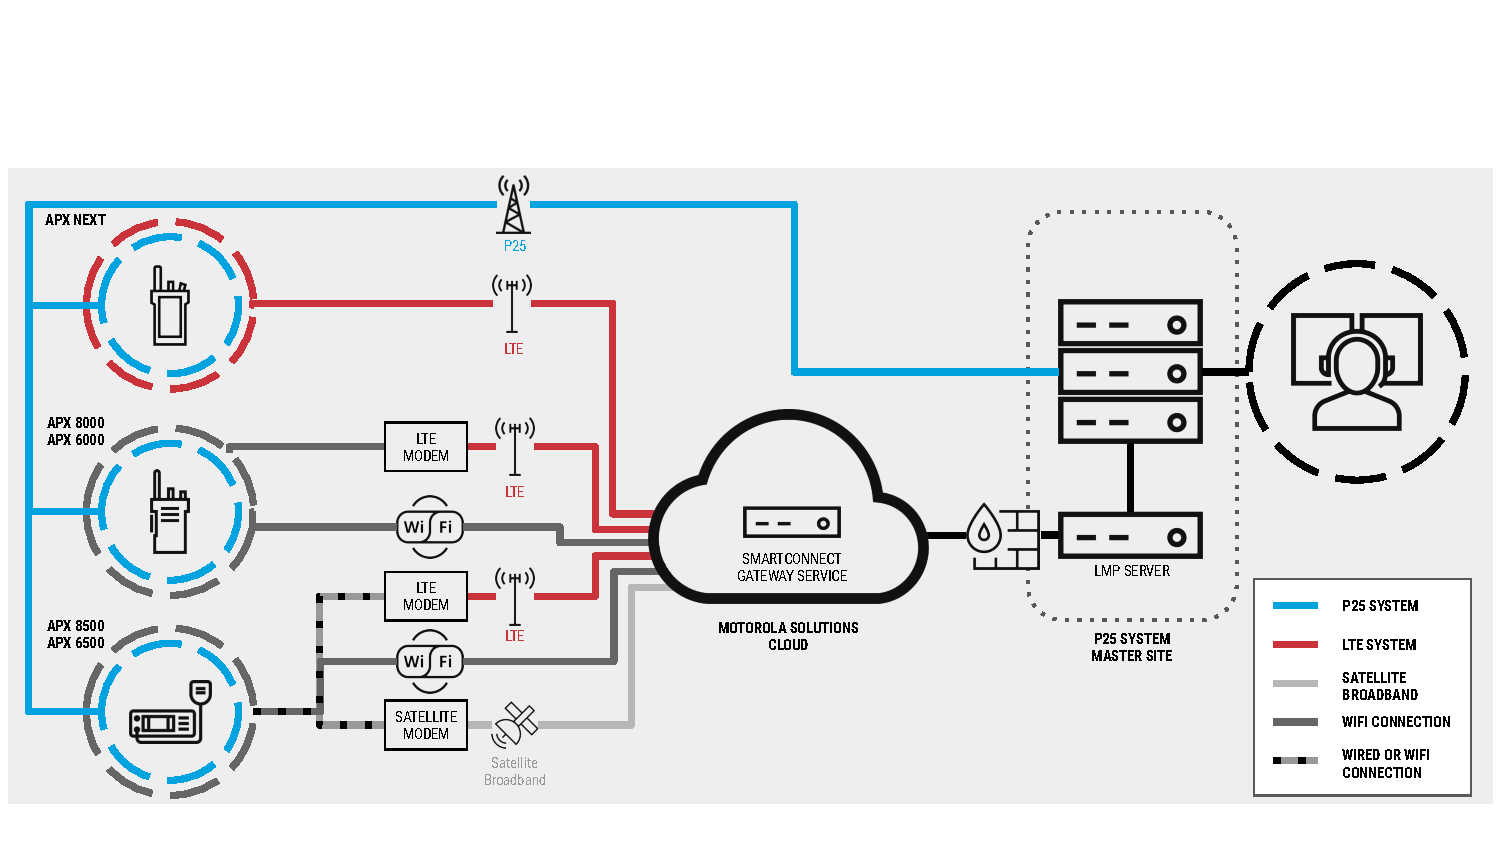
\includegraphics[width=\textwidth]{img/motorola-smart-connect-architecture.pdf}
    \caption{Overview of Motorola two-way radio network showing the various technologies that can be exploited to interconnect push-to-talk radios \cite{apxnextslides}.}
    \label{smart-connect:smart-connect-architecture}
\end{figure}

When a radio utilizes the SmartConnect technology, voice packets are being transferred through the broadband bearer to a cloud-based gateway. This gateway in the cloud connects to the LMR master site. This allows the radios communicating over SmartConnect call back in the LMR system \cite{apxnextslides}.

Therefore, Motorola Solution's SmartConnect helps teams stay connected no matter where they are located by leveraging various means of voice packet transmission.

\section{Software Architecture of SmartConnect}
\label{smart-connect:architecture}

Now let's have a look at the core concepts that form the whole cloud based gateway functionality from the software architecture perspective. 

Having familiarity with the architecture of SmartConnect is important for being able to tackle the anomaly detection problem in an informed way. It gives us a better understanding of what are the weak links that are prone to error about the software.
In this thesis we want to target anomalies based on logs. Knowing the architecture also helps with identifying what parts of the system produce logs that can be collected and extracted information from.

The software follows the \textit{Microservices Architecture} (MSA).
Nadareishvili et al. \cite{nadareishvili2016microservice} define a \textit{microservice} as an independently deployable component of bounded scope that supports interoperability through message-based communication. 

Fowler \cite{fowler2014microservices} understands the microservice architectural style as a way of building a single application by connecting a set of small services. Each of the services runs in its own process and communicates with lightweight mechanisms.

Another attribute of such an architecture is that management of the service is decentralized, therefore it allows for the individual services to be written in various programming languages and use different technologies for storing their data.

A collection of services that communicate together form a \textit{system} \cite{indrasiri2018microservices}.

\subsection{Deployment}

In the analyzed system, the individual services are deployed as Docker\footnote{\url{https://www.docker.com/}} containers in Kubernetes Pods\footnote{\url{https://kubernetes.io/docs/concepts/workloads/pods/}} which are self-standing applications inside of Kubernetes\footnote{\url{https://kubernetes.io/}} clusters.

This approach allows the services to be decoupled as each one resides in its own isolated virtual container.

As described in more detail in Chapter~\ref{data_collection} on Data Collection, the services log each at a different location by default. 
In order to analyze the behaviour of the system holistically, an extra layer for processing logs has to be introduced. SmartConnect, like many others, for this use-case utilizes the Elasticsearch engine that also runs as one of the services in the cluster.

High level view of a Motorola SmartConnect Kubernetes cluster is presented later when discussing the way we deployed our tool for downloading logs from the Elasticsearch service in Figure~\ref{fig:data_collection_elastic}.


\subsection{Elasticsearch}
\label{smart-connect:elastic-search}
Elasticsearch\footnote{\url{https://www.elastic.co/elasticsearch/}} is an open-source, distributed search engine. Gormley and Tong \cite{gormley2015elasticsearch} argue that it can be used for exploring data at unprecedented speed. It is mostly recognized for its exceptional performance on text based data. Operations such as full-text search, structured search and analysis are supported efficiently.
Elasticsearch can also be defined as a NoSQL database since it gathers JSON based \texttt{documents} of a specific \texttt{type} together and multiple \texttt{types} are organized into \texttt{indices}\footnote{\url{https://www.elastic.co/blog/what-is-an-elasticsearch-index}}. 

\subsection{Messaging}
\label{architecture:messaging}
As mentioned earlier, services in an MSA application may be designed in a different way and two services are free to use two dissimilar sets of technologies. That makes the communication within a system more complicated than calling a function - what one would do in a traditional, monolithic architecture.

Two main strategies of passing messages between system's services are \textit{synchronous} and \textit{asynchronous} communication. One of the most common types of synchronous communication is Representational state transfer (REST) \cite{indrasiri2018microservices}.

On the other hand, asynchronous communication promotes autonomy between services as the communicating client does not need to wait for the response. 
For implementation of asynchronous protocols, the concept of a \textit{broker} is introduced. A broker is a centralized entity with high-availability \cite{indrasiri2018microservices}.

In SmartConnect, services are passing values asynchronously. In order to achieve some high-level goal, services form a chain of $1$ or more microservices. Each link of the chain receives an input, processes it and if needed, forwards its output through a broker to another microservice(s) that take(s) this data as input.

For dealing with asynchronous messages, \texttt{RabbitMQ}\footnote{https://rabbitmq.com/documentation.html} brokers are deployed.
\texttt{RabbitMQ} is an open-source publisher/subscriber message broker.

\subsection{Storing Data}
\label{architecture:caching}
In microservices architecture systems, microservices that are immutable and stateless are favoured \cite{indrasiri2018microservices}. 
Therefore, data that the internal state of a microservice comprises of needs to be persisted in storage that is external to memory of a microservice application.

Traditionally, a database is utilized for persisting data externally to the application. However, it is well known that there are major set back when it comes to performance of read/write operations that can be improved by deploying supporting caches \cite{elhardt1984database}.

Performance of the system is fairly crucial as, among others, UDP (user datagram protocol) audio packets of push-to-talk radio calls are being transferred and processed in the system. 
In order to satisfy strict requirements on jitter in the audio signal, a NoSQL data storage Redis\footnote{https://redis.io/} service is running inside of the Kubernetes cluster to serve requests for the stored data rapidly.

\chapter{Literature Review}
\label{chapter:literatureReview}

Before we begin the actual development of our anomaly detection tool, we first needed to establish some core concepts and review the good work that has already been done in this area.

Therefore, in the following sections, we will introduce the notion of anomaly detection. We will present ideas that the reader should be familiar with in order to fully understand anomaly detection techniques and, by extension, our work.

We then explain the three main categories of machine learning - supervised, semi-supervised and unsupervised. We discuss what their distinctive features are when applied in the anomaly detection domain. 
We then go into detail about four different machine learning algorithms and argue why they are the most suitable candidates for our task.

We also explain what we understand by a log, log template, and discuss the most common techniques for log parsing and log-template mining.

We conclude the chapter with an analysis of various log parsing tools. The overview allows us to argue which log parser would be best suited for our application.

\section{Anomaly Detection}
\label{section:anomalyDetectionLiteratureReview}

% The definition of anomaly detection
\textit{Anomaly detection} is a problem of finding patterns in data that do not follow the expected normal behaviour represented by the majority of data points. It follows that defining the normal behaviour is one of the crucial challenges of anomaly detection. 
The unusual patterns are also called \textit{outliers} or \textit{anomalies} and anomaly detection is often called \textit{outlier detection}. 
Outlier was defined by Ord \cite{ORD1996175} as an outlying observation that appears to be significantly different from other members of the sample in which it occurs. 
In other words, the statistical properties of the anomalous data points are not in alignment with the rest of the data. 
Outliers vary by domain and can occur for a variety of reasons, such as fraudulent behaviour in credit card fraud, computer network intrusions, system failures, mechanical failures in industrial applications, deviations due to natural behaviour, or human error. 

Anomaly detection is also related to the term \textit{noise}. Noise is defined as an undesirable phenomenon in data that is not of interest to the analyst but hinders data analysis \cite{cvbakv2009}. Noise is caused by an external factor unrelated to the distribution that generates the data \cite{ggh2017} and leads to excessively complex models with degraded performance \cite{wu2007}. 

In our thesis, we focus on anomaly detection in \textit{time series} data. Time series outlier analysis examines anomalies in the behaviour of data over time \cite{gupta2014}. An outlier in time series data is a data point that does not follow a common behaviour, either a general long-term trend or a tendency of the data to increase or decrease in seasonal patterns.

Originally, outliers were detected manually by the hand of a domain expert. 
Nowadays, the focus of anomaly detection is on automatic detection of anomalous behaviour. 
It has been proven on many occasions that the problem of automatic anomaly detection can be successfully tackled by learning from data \cite{he2016} \cite{wang2017timeseriesanomaly}.
\\
We can divide anomaly detection methods into three broad categories: \textit{supervised}, \textit{semi-supervised} and \textit{unsupervised} anomaly detection. Supervised learning algorithms are trained by examples and require a dataset that is already labeled. Unsupervised methods, on the other hand, do not require any labeled data at all. Semi-supervised methods combine both approaches; in addition, some semi-supervised approaches assume that normal class instances are labeled.

% describe the advantages of unsupervised methods over supervised ones https://reader.elsevier.com/reader/sd/pii/S0167404818306333?token=9C7DC222C83AC3AD33CBF921C2E23508BEA68B59C5336EC0200EF02A1F60DAB2916EEE9D83663EE9029AB30B9C1CC538

\subsection{Supervised Anomaly Detection}
Supervised methods require previously labeled data, where the labels describe whether the behaviour in each data instance is normal or abnormal (anomalous). The main focus of supervised learning methods is then to derive a model from the labeled data that maximizes the discrimination between the classes (normal and anomalous). A drawback of the supervised method is that it can only be trained on the types of anomalies introduced in the training examples. It cannot handle previously unseen anomalies. 

\subsection{Semi-supervised Anomaly Detection} %https://www-users.cs.york.ac.uk/vicky/myPapers/Hodge+Austin_OutlierDetection_AIRE381.pdf.
%https://researchbank.swinburne.edu.au/file/cee84793-6f09-49ce-a099-41451c803b81/1/mostafa_farshchi_thesis.pdf
Semi-supervised learning is defined as a machine learning paradigm that studies how computers, or even natural systems like humans, learn in the presence of both labeled and unlabeled data \cite{zhu2009introduction}.

 
\subsection{Unsupervised Anomaly Detection}
Unsupervised learning, unlike supervised learning, does not require any prior knowledge about the data. One of the main difficulties faced by anomaly detection is unlabeled data. In most cases, logs with labeled anomalies are not available. The process of log annotation would have to be done manually by the experts - developers who are familiar with the system. Along with the growth of data volume, labeling becoms very time consuming. For this reason, in practice, anomaly detection mostly relies on unsupervised learning to deal with unlabeled data. Unsupervised anomaly detection algorithms learn what normal behaviour looks like. Based on these observations, systems based on unsupervised methods detect anomalies as outliers that are significantly different from other examples. Moreover, any type of anomaly can be detected by these systems. Thus, the main difference between supervised and unsupervised learning techniques is that the former focuses on discriminating concept classes, while the latter rather focuses on data characterization \cite{Goernitz_2013}. % They work on the basis of the observation that an abnormal instance usually manifests as an outlier point that is distant from other instances. As such, unsupervised learning techniques, such as clustering, can be applied.
 
\subsubsection*{One-Class Classification}
When it comes to anomaly detection, it is common to use a special method called One-Class Classification (or One-Class Learning) formulated by Tax \cite{tax2002occ}. 
 
In OCC, labels are only provided for instances of the normal class, while labels are not required for classes describing anomalies. In fact, it is discouraged that they occur in the training dataset. There should be so few instances of outliers that they do not form a statistically representative sample of the positive concept, where positive refers to anomalous class \cite{khan_madden_2014}.
 
Thus, in a semi-supervised mode, the model that captures normal behaviour is created and used to identify anomalous behaviour. A class describing normal data is used primarily because it is more readily available, while a labeled dataset that would cover all anomalies is difficult to obtain \cite{cvbakv2009}.
 
Due to the nature of our data, we used unsupervised anomaly detection methods in a one-class manner for this study.

\subsubsection{Isolation Forest}
\label{section:lrIsolationForest}
Isolation Forest or iForest \cite{liu2012isolation} is an ensemble approach for anomaly detection. Majority of existing model-based methods attempt to model normal behaviour, and then a deviation from the normal region that does not fit the model well is considered an anomaly \cite{introToDataMining2005}. Isolation Forest approach, on the other hand, isolates anomalies directly without using the distance from the previously defined normal region. It exploits two properties that can be observed in anomalies. Anomalous instances are the minority of data points and their attribute-values are very different from normal instances. Due to these properties, anomalies are susceptible to a concept called \textit{isolation}, which is the main idea behind Isolation Forests. Liu et al. \cite{liu2012isolation} defined isolation in their research paper as "separation of an instance from the rest of the instances".

Isolation Forest starts by selecting a random attribute and then creates a random partition between the maximum and minimum values of that attribute. This process is applied recursively until all samples are isolated, which can be represented by a binary tree structure (Isolation Tree of iTree). Then, the number of partitions performed to isolate a point is equal to the length of the traversal path from the root node to a terminating node. The iForest is built by adding a given number of iTrees obtained by randomly generated partitions, and their averaged traversal path lengths are then used as a measure of anomaly score. It is easy to see that the isolation of anomaly instances happens closer to the root of the tree, hence the path lengths are also shorter.

Since the anomaly score is the average path length of iTree, which corresponds to an unsuccessful search in the binary search tree, the equation for the anomaly score is derived from the analysis of the binary search tree. Let $n$ be the number of instances in a dataset $X$. The anomaly score $s$ of an instance $x \in X$ is defined as:
 
 \begin{gather}
     s(x, n) = 2^{- \dfrac{E(h(x))}{c(n)}},
 \end{gather}
 
 where $h(x)$ a length of a traversed path from the root node to a terminating node $x$, $E(h(x))$ is the average of $h(x)$ in all isolation trees and $c(n)$ is a normalization factor defined as: 
 
 \[
 c(n) = 
  \begin{dcases}
     c(n) = 2H(n - 1) - (2(n - 1) / n), & \text{if } n > 2\\
     1, & \text{if } n = 2\\
     0, & \text{otherwise}
 \end{dcases} 
 \]
 
where $H(i)$ is the harmonic number estimated by $ln(i) + 0.5772156649$. \\

The Isolation Forest algorithm operates in linear time complexity and is particularly suitable for large and high dimensional datasets due to its low memory requirements. It is proven to be an accurate and effective anomaly detector.

\subsubsection*{Anomaly Detection Forest}
Recently, a variant of the Isolation Forest algorithm has been studied by Sternby et al. \cite{adForest} for the specific use case of Anomaly Detection - Anomaly Detection Forest. It is also commonly referred to as One-Class Isolation Forest. 
It falls under the category of One-Class Classification algorithms.

In their work they claim that the algorithm outperforms the state-of-the-art algorithms Isolation Forest and One-Class Random Forest for the task of anomaly detection in the one-class learning setting. They argue that IF has an intrinsic bias towards labeling similar unusual normal instances as anomalies.

They try to improve that by introducing two new concepts:
\begin{itemize}
    \item \textit{Anomaly leaves} with the aim of catching anomalies with feature values that are not contained
            in the range of the subsample of tree training observations.
    \item \textit{Isolation level}, which is a lower size bound on the training samples in a node during training, and determines when anomaly leaves should be created rather than further subdividing the training samples.
\end{itemize}

Although the results seem promising, we decided not to proceed with this algorithm because the reference implementation is proprietary.
Our goal is to optimize the original IF algorithm so that it performs reasonably well when learning from normal data only.
 
\subsubsection{PCA}
\label{section:lrPCA}
%https://www.usenix.org/legacy/event/sysml08/tech/full_papers/xu/xu.pdf
One problem with high dimensional data is that it is often noisy and even redundant. In such a case, dimensionality reduction is a useful tool to address this problem. Principal Component Analysis (PCA) is one of the most commonly used dimension reduction methods. The reduction is done by projecting the data onto a lower dimensional subspace that captures the "essence" of the data \cite{murphy2013machine}. The similarities and differences in the data become visible in the new coordinate system. 

PCA uses projection methods on a given set of input data points with many input features. Once a PCA model is obtained, a distance from test log entries (either positive or negative) to normal space can be calculated to detect anomalies. Correlations in the original feature space are searched for and the combination of variables that maximizes variance is found to preserve all information with minimal redundancy. A new, more representative and compact feature space is generated. This feature space with lower dimensions is called the \textit{principal components}. The features in the principal components are uncorrelated and ordered by the proportion of the data variance that each feature captures.\\

To put it formally, let's say we have an $m$-dimensional vector $\mathbf{Y} \in \mathbb{R}^n$ with $n$ standardized input features in the original data. The PCA model decomposes $\mathbf{Y}$ into two parts \cite{pca1997}:

\begin{gather}
 \mathbf{Y} = \mathbf{\hat{Y}} + \mathbf{\widetilde{Y}}
\end{gather}

Where $\mathbf{\hat{Y}}$ represents the modeled part of the projection - the selected principal components. $\mathbf{\widetilde{Y}}$ represents the residual part of the projection. The modeled part is obtained by projecting the original data $\mathbf{{Y}}$. The projection is shown in the equation \ref{formula:projection}, where $\mathbf{P} \in \mathbb{R}^{n \times k}$ is the PCA loading matrix, $k$ is the number of principal components, and the matrix $\mathbf{C = \mathbf{PP}^T}$ is a projection matrix. 
Thus, $\mathbf{C}$ is a matrix for a projection of the original data onto a model space, so called normal space $S_d$ with $n$ dimensions.

\begin{gather}
     \mathbf{\hat{Y}} = \mathbf{P}\mathbf{P}^T\mathbf{Y} = \mathbf{CY}
    \label{formula:projection}
\end{gather}

The remaining $(n - k)$ dimensions form the residual subspace, also called the anomaly space $S_a$. $\mathbf{\widetilde{Y}}$ corresponds to the projection of $\mathbf{Y}$ onto the residual subspace $S_a$. The equation \ref{formula:residualProjection} shows how the $\mathbf{\widetilde{Y}}$ can be mathematically computed.  

\begin{gather}
     \mathbf{\widetilde{Y}} = (\mathbf{I - C})\mathbf{Y} = \mathbf{\widetilde{C}Y}
    \label{formula:residualProjection}
\end{gather}
 
% How is it applied in anomaly detection.
When PCA is applied to an anomaly detection task, for each new input its projection is computed. An anomaly can be detected with a large change in variable correlation if normal behaviour is not preserved. If this is the case, the projection on the residual subspace $S_a$ is increased. As a side effect, unusual values of the magnitude of $\mathbf{\widetilde{Y}}$ can be observed. In other words, an anomalous vector is farther away from the normal space $S_d$.\\

The squared prediction error (SPE) in the equation \ref{formula:predictionError} is a useful evaluation metric to measure the distance from $S_d$.
 
 \begin{gather}
     SPE = \parallel \mathbf{\widetilde{Y}} \parallel^2  = \parallel \mathbf{\widetilde{C}Y} \parallel^2
    \label{formula:predictionError}
\end{gather}

SPE is used as an anomaly score: The higher the prediction error, the more anomalous the data instance. A process block is considered an anomaly if:

\begin{gather}
     SPE \leq \delta^2
\end{gather}

where $\delta^2$ is a threshold for the error. A standard implementation of the threshold  $\delta^2$ in anomaly detection is based on the \textit{Q-statistics} proposed by Jackson \cite{pcaJackson1979}. According to this, an anomaly is detected if the following holds:

\begin{gather}
    SPE = \parallel \mathbf{\widetilde{Y}} \parallel^2 > Q_{\alpha} 
\end{gather}
 
where $Q_{\alpha}$ denotes a Q-value statistics providing a $(1 - \alpha)$ confidence level. 

\subsubsection{Invariants Mining}
\label{section:lrInvariantMining}
 
A linear program invariant is a predicate that always holds the same value under different normal executions - different workloads or inputs. Lou et al. were the first to propose automatic anomaly detection by mining linear invariants from logs \cite{lou2010}. It is based on the assumption that log sequences provide enough information about the execution paths of the system. Linear invariants are extracted from execution path properties by analyzing log sequences that follow workflow logic. The ideal candidate for the dataset for mining invariants are positive log samples. We know that some examples of linear relationship between logs can also be found in the Motorola SmartConnect system dataset. 
There are steps in the call logic, such as subscribing to a call group, calling, and unsubscribing that are recorded and could potentially be exploited for anomaly detection. The occurrence of the above messages in pairs is an expected normal behaviour. Therefore, the number of these event types should be the same in one execution of the program. 

We can formally define a linear invariant as a linear equation:

\begin{gather}
    a_0 + a_1 x_1 + ... + a_m x_m = 0,
\end{gather}

where $x_i$ is the event count of the event type with identifier $i$ and $\theta = [a_0, a_1, ... a_m]^T$ is the vector representing the coefficients. It holds that: 

\begin{gather}
\mathbf{X} \theta = 
\begin{bmatrix}
1 & x_{11} & x_{12} & \hdots & x_{1m}\\
1 & x_{21} & x_{22} & \ddots & x_{2m}\\
1 & \vdots & \vdots & \vdots &\vdots \\
1 & x_{n1} & x_{n2} & \hdots & x_{nm}\\
\end{bmatrix}
\theta = 0
\end{gather}

Log datasets that contain information about the specific execution flow, such as session ID or job ID, are best suited for invariant mining because they reflect the execution workflow of that session or job. An execution workflow consists of smaller elementary units called elementary workflow structures, such as \textit{sequential}, \textit{branched}, \textit{joint}, or \textit{looping} structures. For example, in the execution flow shown in Figure \ref{figure:invariantMiningExecutionFlow}, we can see a sequential workflow structure from A to B, a branched workflow structure from B to C or D, and a shared workflow structure from C to E or from D to E. Multiple execution instances of the program may run concurrently, they may execute different branches of the flow, and the logs produced may intersperse. In any case, the following should hold:

\begin{align}
    c(A) &= c(B) = c(E) \\
    c(B) &= c(C) + c(D),
\end{align}

where $c(x)$ denotes the number of log messages of event type $x$. 

Intuitively, invariant mining reveals the linear relationships between the logs and their respective events in the program workflows, e.g., the invariant $c(B) = c(C) + c(D)$ tells us that there could be a branched or shared elementary structure in the workflow. 

In invariant mining, anomalies are detected by checking the invariant rules, which are broken by some log events. This not only detects an anomaly, but we can also see the logical reasoning behind an anomaly by looking at the invariants.

\begin{figure}\centering
	\begin{tikzpicture} [
    serviceNode/.style={circle,draw=customDarkBlue,fill=white,thick,inner sep=0pt,minimum size=8mm, thin},
    condition/.style={diamond, thin, draw=black,fill=white,inner sep=0pt,minimum width=3cm, minimum height=1cm, draw=customBlue},
    arrow/.style={thin, -latex, color=customGrey}
]
    % output invisible node
    \node[serviceNode] (E) at (10, 3) {\tiny E};
    \node[serviceNode] (D) at (8, 1) {\tiny D};
    \node[serviceNode] (C) at (8, 5) {\tiny C};
    \node[condition] (cond) at (6, 3) {\small \textcolor{customDarkBlue}{Condition}};
    \node[serviceNode] (B) at (2, 3) {\tiny B};
    \node[serviceNode] (A) at (0, 3){\tiny A};
    
    \draw [arrow] (A) -- (B);
    \draw [arrow] (B) -- (cond);
    \draw [arrow] (cond) |-  node[anchor=south] {\textcolor{black}{\small $x = 0$}} (C);
    \draw [arrow] (cond) |- node[anchor=north] {\textcolor{black}{\small $x \neq 0$}} (D);
    \draw [arrow] (C) -- (E);
    \draw [arrow] (D) -- (E);
\end{tikzpicture}
	\caption{An example of an execution flow of a program that sequentially executes $A$ and $B$, then based on a given condition branches and proceeds with either execution of $C$ or $D$, and finally runs $E$.}
	\label{figure:invariantMiningExecutionFlow}
\end{figure}

The workflow of the invariant mining anomaly detection approach is partially identical to other methods described in our thesis. Unstructured free-form log messages representing normal behaviour are parsed into a structured form. The second step requires grouping messages. Grouping is performed for log messages that contain cogenetic parameters (e.g., session ID). An event count vector is generated for each group. Next, sparse integer valued invariants are discovered on the event count vectors using a greedy invariant mining algorithm. Finally, the learned invariant rules are used to detect anomalies.

\subsubsection{Log Clustering}
 \label{section:lrLogClustering}

Clustering-based approaches to anomaly detection rely on an intuitive principle. Normal data samples generate clusters, and data that do not conform to these clusters (they are far from them) are considered as anomalies. LogCluster is a tool developed by Lin et al. \cite{logCluster2016} that enables unsupervised anomaly detection by clustering log sequences that are similar. 

LogCluster consists of two phases: \textit{construction} phase and \textit{production} phase. 

\subsubsection*{Construction Phase}
The construction phase can again be divided into four steps: Log vectorization, log clustering, extraction of representative log sequences, and recurrence checking.

\begin{enumerate}
    \item \textbf{Log vectorization}:In the log vectorization step, unstructured log messages are parsed into numeric vectors by abstracting log events. Then, log sequences are obtained by grouping logs with the same task ID and vectorization by counting the frequency of the event ID in the log sequence. Event ID frequency is further weighted using the Inverse Document Frequency based weighting. The Inverse Document Frequency (IDF) weighting technique is also used in our research and we describe it in more detail in Section \ref{subsection:features}.
    
    While in our research we combine IDF weight with event type frequency per log sequence, in LogCluster they use \textit{contrast-based} weighting. The intuition behind the contrast-based weighting is the observation that an event that occurs in both the test and production environments is less discriminative for anomaly detection than an event that appears only in the production environment. Events that occur only in the production environment are assigned a higher weight because they are assumed to better reflect failures.
    
    \item \textbf{Log clustering}: The vector representation of log sequences allows the computation of distances between two vectors $A$ and $B$ of dimension $n$. The similarity measure used in LogCluster is the cosine similarity:

    \begin{align*}
        similarity(A, B) = cos(\theta) &= \dfrac{A \cdot B}{\|A \| \|B\|} \\
        &= \dfrac{\sum_{i=1}^n A_i B_i}{\sqrt{\sum_{i=1}^n A_i^2} \sqrt{\sum_{i=1}^n B_i^2}}
    \end{align*}
    
    Normal and anomalous log sequences are partitioned into clusters using the agglomerative hierarchical clustering technique \cite{ahc1969}. Initially, each log sequence belongs to its own cluster. The closest pair of clusters is then merged. The metric for measuring the distance between two clusters is defined as the maximum distance of all pairs of elements between two clusters. The stopping criterion for agglomerative hierarchical clustering is given by a distance threshold $\theta$, which is empirically determined but initialized to $0.5$. An example in Figure \ref{figure:hierarchicalClustering} shows the process of producing clusters with agglomerative hierarchical clustering.
    
    \item \textbf{Representative log sequence extraction}: In this step, one representative log sequence called \textit{centroid} must be selected for each of the clusters obtained. A centroid is a log sequence with a minimum score computed for each log sequence in the cluster as the average distance from the rest of the log sequences in the same cluster. Formally, we compute the score for a log sequence $L_i$ in a cluster as follows:
    
    \begin{align*}
        score(i) = \dfrac{1}{m - 1} \sum_{j = 1}^m (1 - similarity(L_i, L_j))
    \end{align*}
    
    where $m$ is the number of log sequences in the cluster.
    
    \item \textbf{Recurrence checking}: In the next and final step of the construction phase, each of the clusters is checked to see if it is a recurrent cluster by querying a knowledge base. The knowledge base stores the centroids of the log clusters from the past executions. If a cluster is not considered a recurrent failure, it is returned to the engineers to be manually examined.
\end{enumerate}

\begin{figure}\centering
	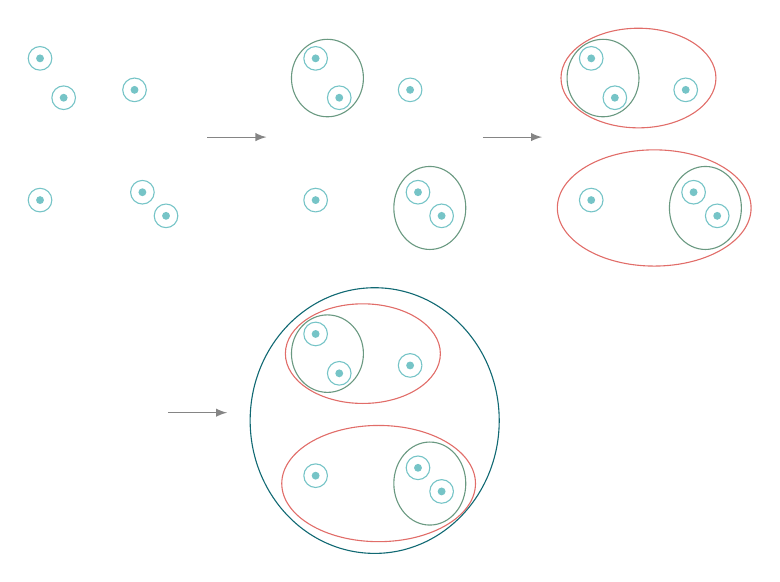
\begin{tikzpicture} [
    object/.style={circle,fill=customBlue,inner sep=0pt,minimum size=1mm, thin},
    singleCluster/.style={circle,draw=customBlue,inner sep=0pt,minimum size=3mm, thin},
    doubleCluster/.style={ellipse, draw=customGreen, thin},
    threeCluster/.style={ellipse, draw=customRed, thin},
    fourCluster/.style={ellipse, draw=customDarkBlue, thin},
    arrow/.style={thin, -latex, color=customGrey}
]
    % 1
    \node[singleCluster] (aCluster) at (0, 0) {};
    \node[object] (a) at (0, 0) {};
    
    \node[singleCluster] (bCluster) at (0.3, -0.5) {};
    \node[object] (b) at (0.3, -0.5) {};
    
    \node[singleCluster] (cCluster) at (1.2, -0.4) {};
    \node[object] (c) at (1.2, -0.4)  {};
    
    \node[singleCluster] (dCluster) at (1.3, -1.7) {};
    \node[object] (d) at (1.3, -1.7)  {};
    
    \node[singleCluster] (eCluster) at (1.6, -2) {};
    \node[object] (e) at (1.6, -2)  {};
    
    \node[singleCluster] (fCluster) at (0, -1.8) {};
    \node[object] (f) at (0, -1.8)  {};
    
    \node[draw=none] (arrow1S) at (2, -1) {};
    \node[draw=none] (arrow1E) at (3, -1) {};
    \draw [arrow] (arrow1S) -- (arrow1E);
    
    % 2
    \node[singleCluster] (aCluster) at (3.5, 0) {};
    \node[object] (a) at (3.5, 0) {};
    
    \node[singleCluster] (bCluster) at (3.8, -0.5) {};
    \node[object] (b) at (3.8, -0.5) {};
    
    \draw[doubleCluster] (3.65, -0.25) ellipse (13pt and 14pt);
    
    \node[singleCluster] (cCluster) at (4.7, -0.4) {};
    \node[object] (c) at (4.7, -0.4)  {};
    
    \node[singleCluster] (dCluster) at (4.8, -1.7) {};
    \node[object] (d) at (4.8, -1.7)  {};
    
    \node[singleCluster] (eCluster) at (5.1, -2) {};
    \node[object] (e) at (5.1, -2)  {};
    
    \draw[doubleCluster] (4.95, -1.9) ellipse (13pt and 15pt);
    
    \node[singleCluster] (fCluster) at (3.5, -1.8) {};
    \node[object] (f) at (3.5, -1.8)  {};
    
    \node[draw=none] (arrow1S) at (5.5, -1) {};
    \node[draw=none] (arrow1E) at (6.5, -1) {};
    \draw [arrow] (arrow1S) -- (arrow1E);
    
    % 3
    \node[singleCluster] (aCluster) at (7, 0) {};
    \node[object] (a) at (7, 0) {};
    
    \node[singleCluster] (bCluster) at (7.3, -0.5) {};
    \node[object] (b) at (7.3, -0.5) {};
    
    \draw[doubleCluster] (7.15, -0.25) ellipse (13pt and 14pt);
    
    \node[singleCluster] (cCluster) at (8.2, -0.4) {};
    \node[object] (c) at (8.2, -0.4)  {};
    
    \draw[threeCluster] (7.6, -0.25) ellipse (28pt and 18pt);
    
    \node[singleCluster] (dCluster) at (8.3, -1.7) {};
    \node[object] (d) at (8.3, -1.7)  {};
    
    \node[singleCluster] (eCluster) at (8.6, -2) {};
    \node[object] (e) at (8.6, -2)  {};
    
    \draw[doubleCluster] (8.45, -1.9) ellipse (13pt and 15pt);
    
    \node[singleCluster] (fCluster) at (7, -1.8) {};
    \node[object] (f) at (7, -1.8)  {};
    
    \draw[threeCluster] (7.8, -1.9) ellipse (35pt and 21pt);
    
    \node[draw=none] (arrow1S) at (5.5, -1) {};
    \node[draw=none] (arrow1E) at (6.5, -1) {};
    
     % 4
    
    \node[draw=none] (arrow1S) at (1.5, -4.5) {};
    \node[draw=none] (arrow1E) at (2.5, -4.5) {};
    \draw [arrow] (arrow1S) -- (arrow1E);
    
     % 5
    \node[singleCluster] (aCluster) at (3.5, -3.5) {};
    \node[object] (a) at (3.5, -3.5) {};
    
    \node[singleCluster] (bCluster) at (3.8, -4) {};
    \node[object] (b) at (3.8, -4) {};
    
    \draw[doubleCluster] (3.65, -3.75) ellipse (13pt and 14pt); \draw[threeCluster] (4.1, -3.75) ellipse (28pt and 18pt);
    
    \node[singleCluster] (cCluster) at (4.7, -3.9) {};
    \node[object] (c) at (4.7, -3.9)  {};
    
    \node[singleCluster] (dCluster) at (4.8, -5.2) {};
    \node[object] (d) at (4.8, -5.2)  {};
    
    \node[singleCluster] (eCluster) at (5.1, -5.5) {};
    \node[object] (e) at (5.1, -5.5)  {};
    
    \draw[doubleCluster] (4.95, -5.4) ellipse (13pt and 15pt);
    \draw[threeCluster] (4.3, -5.4) ellipse (35pt and 21pt);
    
    \node[singleCluster] (fCluster) at (3.5, -5.3) {};
    \node[object] (f) at (3.5, -5.3)  {};
    
    \draw[fourCluster] (4.25, -4.6) ellipse (45pt and 48pt);
    
    
\end{tikzpicture}
	\caption{A visualization of agglomerative hierarchical clustering. At the beginning, each object is a cluster. In each step, the two closest clusters are merged. The process is finished when the maximum distance between the clusters reaches the threshold $\theta$. This figure illustrates the case without a stopping criterion, where the process terminates when all objects are in one cluster.}
	\label{figure:hierarchicalClustering}
\end{figure}

%https://netman.aiops.org/~peidan/ANM2019/6.LogAnomalyDetection/LectureCoverage/2016ICSE_Log%20Clustering%20based%20Problem%20Identification%20for%20Online%20Service%20Systems%20.pdf page 5

\subsubsection*{Production Phase}
In the production phase, logs are collected from the actual production environment (or more generally, the monitored environment). The process is then the same as in the construction phase: the logs are vectorized into log sequences and the log sequences are clustered. For each cluster, a representative is extracted. Then, the algorithm checks if all the representatives fall under one of the clusters seen earlier in the knowledge base. After that, engineers are required to manually examine the log sequences that have not been seen before for anomalies. After resolution, the knowledge base is updated with new clusters.
 
\section{Log Parsing}

The time series data we are working with is a sequence of \textit{logs} produced by a development or production system. 
\textit{Log} is a textual trace of variable length runtime information designed to be easily readable for humans.

Let's consider a set of log entries produced by a particular system. Each log entry is recorded by the service that performs the action described in the log. In general, a log typically contains a \textit{timestamp} (which records \textit{when} a particular event occurred) and a \textit{message} (free-form text describing the event). A log may also contain additional metadata, such as \textit{log level} (log severity describing how important a log message is, e.g., INFO, DEBUG, ERROR, WARN) or \textit{program name} (name of the node that caused the event). An example of properties in a log entry generated by Motorola SmartConnect is described in Appendix \ref{appendix:log-properties}.\\

In our thesis, we consider only the \textit{message} and \textit{timestamp} parts of the log. Since log messages are usually written into the source code by different developers, we defensively assume that logs contain only these two properties. \textit{Timestamp} is added by default by the majority of the most commonly used logging frameworks \cite{log4j:example} \cite{serilog:example} \cite{python_log:example}, so we will assume that \textit{timestamp} is present along with the necessary \textit{message}.

According to Legeza et al. \cite{structured_logging}, structured logging is an approach where each log entry is represented in a format that can be easily processed by a computer, such as XML, JSON, or other well-defined structures. When this is not the case, we call logs that do not follow a strict format \textit{unstructured}.

Most commonly, \cite{log4j:example} \cite{serilog:example} \cite{python_log:example}, \textit{timestamp} comes as the first field of the log line, so can be easily parsed even if the log does not meet the definition of \textit{structured} log.

However, even with \textit{structured} logs, there is a part we call \textit{message} that contains the contents of the log and answers questions like "what", "why", and "what's going to happen next" \cite{structured_logging}.\\

It can be seen that each log message consists of a \textit{constant} part and a \textit{variable} part. Both can possibly be empty and the \textit{variable} part may consist of zero or more \textit{variables}.
As the names imply, the constant part remains the same throughout the execution of the code, while the variable parts may change from one run to another.\\
The \textit{constant} part can be understood as the part that a developer explicitly writes in plain text and the variables are generated during the execution of a system based on the state of the placeholder variables in the code.\\

Let's define an \textit{event type} as a class of logs, where each of the logs belonging to that class has a \textit{message} that follows the same \textit{template}. This means that all of the logs in the same class have identical constant part and their variable part consists of an identical number of variables of the same data types in the same positions.

Two different messages may contain different string values when they track the same event under different circumstances. Circumstances are described by values that form the \textit{variable} part of a log message. Variables are inserted dynamically into the plain message text, e.g. by string interpolation\footnote{\url{https://docs.microsoft.com/en-us/dotnet/csharp/language-reference/tokens/interpolated}}.

To have a tool to generalize a log message template in technical terms, we refer to a log template as a regular expression. The expression is encoded as a string with the constant part and regular expressions describing the variables and possibly their data types.

The purpose of log parsing is to obtain a structured input for further log analysis by extracting these event types from the natural language messages into categories.
In other words, the goal is to associate an event type with each log that the system produces.\\

Now let's look at an example of what the log entry we just defined looks like.
When a programmer writes code, he calls a logging framework at places where something noteworthy happens. The lines that call such a framework are shown in Listing~\ref{lst:logging_code}.\\

\begin{lstlisting}[language=elixir, caption={Example of how logging is done in source code}, captionpos=b, label={lst:logging_code}]
Log.info("Cached default value,tenant: 
            #{inspect(tenant_id)}, param key: #{key}")
\end{lstlisting}
\\
This line of code may, as we pointed out earlier, result in distinct log messages, as shown in Listing~\ref{lst:log_messages}.\\

\begin{lstlisting}[label={lst:log_messages}, caption={Possible outputs of the code in Listing~\ref{lst:logging_code}}, captionpos=b]
Cached default value, tenant: 12556, param key: 12
Cached default value, tenant: 45, param key: 4
Cached default value, tenant: 789, param key: 54
Cached default value, tenant: 12556, param key: 78
\end{lstlisting}

Importantly, all log messages in Listing~\ref{lst:log_messages} describe the same event type, where a default value was written to the cache and the variable part describes details of the changed context, which was different. Therefore, they are of the same event type and follow the same template. \\

Now it is easy to derive a log template. For example, a template for the messages we saw in Listing~\ref{lst:log_messages} can be described by the template shown in Listing~\ref{lst:log_message_template}\\

\begin{lstlisting}[label={lst:log_message_template}, caption={Template for log messages in Listing~\ref{lst:log_messages}, regular expressions are shown in blue.}, captionpos=b]
Cached default value, tenant: <@\textcolor{blue}{[0-9]+}@>, param key: <@\textcolor{blue}{[0-9]+}@> 
\end{lstlisting}

Therefore, we say that two logs have the same event type if their messages match the same log message template. Now that we have an idea of what the goal of log parsing is, let's take a closer look at the process and technique of \textit{log parsing}. We think of log parsing as a superset of the \textit{log-template mining} process.\\

\subsection{Log-Template Mining}\label{log_template_mining}
% Now let's look into how we categorize logs from our system into event types.

   % \subsection{Log-Template Mining}
    % MANUAL 
    % AUTOMATED - OFFLINE
    %           - ONLINE
\textit{Log-template mining} is a process of extracting an information about the event from unstructured log messages by separating its constant and its variable parts. High accuracy of log parsing is of great importance for effective log mining \cite{logParsingEvaluation2016}. For this reason, we will give a brief overview and evaluation of different log parsing approaches that have been proposed and used in the past. \\
    
Originally, log parsing was based on regular expressions written manually by developers themselves. As we can assume, manual parsing is not an ideal solution for several reasons. Indeed, designing regular expressions by hand is a very error-prone and time-consuming process, as the size of the code may be too large for a single developer. Moreover, the ever-increasing complexity of modern software systems makes it recognizably more difficult to update and maintain these regular expressions. According to Xu et al. \cite{xu2009}, the number of new logs introduced into Google's newly developed system amounts to about a hundred per month. \\
\\
As an alternative to writing regular expressions, several automated methods have been proposed that typically operate in one of two modes. Either in \textit{online} (\cite{drain2017}) or \textit{offline} (\cite{vaarandi2003}, \cite{logsig2011}, \cite{Makanju2009ALA}) mode. Most of the current log parsers work offline, which means that they need to have a full collection of logs available before the actual log processing takes place. This implies that the entire log dataset must be loaded into memory. One such example is a study by Xu et al. \cite{xu2008}, in which they use the source code and a search function in a text editor to search for each occurrence of the logging function. From each log in the file, they extract a regular expression and compare them to find the best match. The disadvantage of this approach is that it is not always possible to have access to the source code, as is the case when using third-party libraries, etc. On the other hand, online log parsing methods process logs immediately when they arrive in a stream. \\
According to the log parsing technique, parsers can be classified into four main groups, including \textit{Clustering}, \textit{Frequent Pattern Mining}, \textit{Heuristic}, and \textit{Fixed Depth Tree} based methods. In the following, we will present more details and an example of a representative of each of these methods, with the overall overview available in Table~\ref{tab:logParsers}.\\

\subsection{Log Parsing Techniques} \label{log_parsing_techniques}
    
\subsubsection*{Clustering} 
 A popular solution to this problem is to use data clustering algorithms. Data clustering algorithms are used in data mining or machine learning, where the set of objects is divided into groups called clusters. Objects in each cluster are similar to each other and as dissimilar as possible to objects from other clusters \cite{vaarandi2003}. An example of this approach is the LogSig \cite{logsig2011} algorithm based on message signatures. It consists of three steps:

\begin{enumerate}
    \item \textit{Term pair generation}. Each log message is converted into a set of pairs of terms. In other words, a pair is formed from every two words in a log message, while maintaining the order of the words. An example of such term pair generation shown in LogSig \cite{logsig2011} is a log message:
    
    \begin{verbatim}
    2010-05-02 11:34:06 Command: mkdir ".indexes"
    \end{verbatim}
    
    Then its corresponding generated set of term pairs is: \\
    \begin{verbatim}
    {2010-05-02, 11:34:06}
    {2010-05-02, Command:}
    {2010-05-02, mkdir}
    {2010-05-02, ".indexes"}
    {11:34:06, Command:}
    {11:34:06, mkdir}
    {11:34:06, ".indexes"}
    {Command:, mkdir}
    {Command:, ".indexes"}
    {mkdir, ".indexes"}
    \end{verbatim}

    \item \textit{Log messages partition}. The goal of the second step of LogSig is to use the word pairs to find a partitioning of the log messages into clusters, maximizing the objective function. The algorithm iterates over the messages, moving messages between clusters to increase the potential value of the objective function. The number of clusters is predefined. 
    
    \item \textit{Message Signature Construction}. The final step of the algorithm constructs the message signature based on identified common pairs for each cluster.
\end{enumerate}
    
\subsubsection*{Frequent Pattern Mining} 
Vaarandi \cite{vaarandi2003} presented a clustering algorithm for finding frequent patterns in logs with his tool SLCT (Simple Log File Clustering Tool). A \textit{frequent pattern} is defined as a set of elements that occur frequently in a data set \cite{zhlhxzl2018}. As we described earlier, we can also think of event templates as a set of constants that occur frequently in log messages. SLCT reformulates the problem of finding event templates as a problem of mining frequent itemsets. The algorithm consists of three steps, with two passes over the data. The algorithm requires a threshold of support, which is set by the user beforehand. 

    \begin{enumerate} 
        \item During the first step (data summarization), the algorithm first performs a pass to build a summary vector from words and their frequencies. After the summary vector is created, a vocabulary is constructed. To optimize the size of the vocabulary, only frequent words (dense 1-regions) are stored. A word is considered frequent if it occurs at least $N$ times in the dataset, where $N$ is the user-specified threshold for support. This step is a modification of the Apriori algorithm for finding frequent itemsets \cite{Agrawal94fastalgorithms}. 
        
        \item In the second step, another pass is made over the data to assemble all cluster candidates into a candidate table. The entire dataset is processed to form a cluster candidate from the line if a combination of the dense 1-regions occurs on the line. If the cluster candidate exists, it is inserted into the table with incremented support value. Otherwise, it is inserted into the table with support value $1$. 
        
        \item In a final step, the cluster candidates are inspected, and all candidates whose support values are equal to or greater than the support threshold are reported as clusters.
    \end{enumerate}

    
\subsubsection*{Heuristics}
IPLoM, proposed by Makanju et al. \cite{Makanju2009ALA}, is an example of a heuristics-based log parsing method. IPLoM stands for \textit{Iterative Partitioning Log Mining}, where their algorithm partitions the log messages into their respective clusters through a 3-step hierarchical partitioning process. In the final 4th stage, IPLoM generates discovered clusters and a line format describing each cluster. We will describe each step in more detail.\\

\begin{enumerate}
    \item \textit{Partition by event size}. The first step of IPLoM applies an event size heuristics based on the assumption that log messages of the same event type have the same event size (number of tokens). The result is a partitioning of log messages into groups of equal length, e.g. \textit{"Connection from 255.255.255.255"} and \textit{"Connection from 0.0.0.0"} both contain $3$ tokens and would end up in the same cluster. The cases where events with different event sizes belong to the same cluster are handled in post-processing.
    
    \item \textit{Partition by token position}. The next step assumes that the tokens at the same position in the log message that have the least number of unique words are likely to contain constants. Then, the heuristics works to find the token position with the lowest number of unique values and further splits each cluster based on the unique values at that position. 
    
    \item \textit{Partition by searching for bijection}. The final partitioning step is based on searching for bijective (one-to-one) relationships between the set of unique tokens in two token positions. If a bijective relationship is found between two elements in the sets of tokens, log messages will be separated into new partitions at the corresponding token positions. The heuristics works as follows: The number of unique tokens at each token position and the most frequent number of unique tokens greater than $1$ are determined. The two token positions with the highest number of tokens are chosen. The idea is that the most frequent token count can indicate the number of event types. For example, in log messages:\\ 
    \texttt{Command has completed successfully} \\ 
    \texttt{Command has been aborted} \\ 
    \texttt{Command failed on starting}, \\ 
    first position of the token has one unique token \{Command\}, the second position has two unique tokens \{has, failed\}, the third position has three unique tokens \{completed, been, on\} and the final fourth position also has three unique tokens \{successfully, aborted, starting\}. Therefore, the tokens at positions three and four, e.g. "completed" and "successfully", are in a $1-1$ bijective relationship with "been" and "aborted", since all lines containing "completed" in position three contain "successfully" in position four and vice versa. There is also a $1-M$ relationship with the tokens "Command", "completed", "been", and "on" because all lines containing "Command" also contain "completed", or "been", or "on" at position three. Another type of relationship is an $M-1$, which works in reverse to the previous scenario. The last type of relationship is $M-M$. This occurs in our example when positions two and three are chosen by the heuristics. \\ Therefore, another heuristics is implemented to handle the case of $1-M$ and $M-1$ relationships. 
    
    \item \textit{Discover message type descriptions (line formats) from each partition}. In this step, the algorithm is terminated and descriptions of clusters or line formats should be discovered.
\end{enumerate}

    \subsubsection*{Fixed-depth tree}\label{fixed_depth_tree}
    Drain \cite{drain2017} uses a parse tree with a fixed-depth structure to represent log messages and then partition them into groups that describe event types efficiently. Drain parses raw log messages individually from streams and does not require an offline preprocessing step, so it works in an online manner.\\ The structure of a parse tree is shown in \ref{parseTreeDrain}. The node in the top layer is the \textit{root node} of the parse tree and the nodes in the bottom layer are called \textit{leaf node}. Nodes between the first and last layer are called \textit{internal nodes}. Each path in the parse tree ends with a leaf node that stores a list of log groups. The depth of the tree is fixed by a predefined parameter \textit{depth}. 
    
        \begin{figure}[htbp]
            \centerline{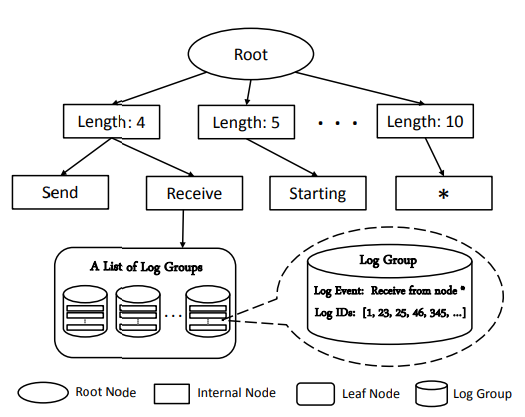
\includegraphics[scale=.5]{img/parse-tree-drain.PNG}}
            \caption{Structure of a simple parsing tree of depth $3$ in Drain \cite{drain2017}.}
            \label{parseTreeDrain}
        \end{figure}
        
    The algorithm consists of five steps: 
    
    \begin{enumerate}
        \item \textit{Preprocess by Domain Knowledge}. According to the empirical study on log parsing methods by He et al. \cite{logParsingEvaluation2016}, preprocessing improves parsing accuracy. Thus, when a new raw log message arrives, Drain will preprocess it with regular expressions provided by the user based on domain knowledge before constructing the actual parse tree. This may include frequently used variables, such as IP address, and any matched tokens will be removed. 
        
        \item \textit{Search by Log Message Length}. The next step is to build the parsing tree. The process is based on the assumption that log messages with the same log event can have the same log message length. Starting from the root node, each node in the first layer represents log groups whose log messages have different lengths. The message length is specified by the number of tokens. Cases where log messages with the same log event have different lengths can be handled by post-processing. For example, the path to the preprocessed log message \texttt{Packet has been sent} to a first layer node would be \textit{Length: 4}.
        
        \item \textit{Search by Preceding Tokens}. In the third step, the parsing tree is traversed to a leaf node in the second layer. In this step, it is assumed that the first tokens in a log message are likely to be constants. For example, in the log message \texttt{Packet has been sent}, the tree is traversed from the first layer node \textit{Length: 4} to the leaf node containing the internal node \textit{Packet}, since "Packet" is considered a constant. Therefore, the second layer contains nodes with unique first words. Depending on the \textit{depth} of the tree, there are more internal nodes which search by the tokens at the first, second, third... etc. position. However, sometimes a variable word may appear in the initial positions, such as \texttt{120 bytes received}. This is solved by considering only tokens that do not contain digits. If a token contains a digit, it matches a special internal node \textit{"*"}. 
        \item \textit{Search by Token Similarity}. After step 3, lists of log groups are contained in leaf nodes. Each log group has \textit{log event} and \textit{log IDs}. Log event is the template that describes the log messages of the group, and log IDs are the log IDs of the log messages in that group. Each log group contains log messages of the same length that start with the same word. In this step, Drain calculates the similarity between the log message and the log event of each log group. The similarity is calculated over each token position. The highest similarity score is compared to a predefined similarity threshold, which indicates whether the given log group is suitable.
        \item \textit{Update the Parse Tree}. In the last step, the log ID of the current log message is added to the most suitable log group from step $4$ and log event in the log group is updated (different tokens are replaced by wildcards *).
    \end{enumerate}

    \subsection{Summary} \label{parser_summary}
    In this section, we presented an overview of automated log parsing techniques and their representative tools. Table \ref{tab:logParsers} provides a summary of all log parsing tools we have reviewed in this paper. The tools are compared from different aspects that we considered important for our use case. \textbf{Mode} denotes the online or offline mode, while \textbf{Method} denotes the log parsing technique used by the tool. \textbf{Preprocessing} describes whether an additional manual preprocessing step is required. \textbf{Performance} categorizes tools into three levels based on their efficiency: high, medium, and low, as proposed in \cite{zhlhxzl2018}. Finally, it is of great importance for practical use that log parsing tools are freely available. Therefore, the last column is devoted to the \textbf{Open Source} characteristics of the existing tools.
    
    \begin{table}[t]
    \centering
    \resizebox{\textwidth}{!}{\begin{tabular}{|c|c|c|c|c|c|c|}
    \hline
    \textbf{Log Parsing Tool} & \textbf{Year} & \textbf{Mode} & \textbf{Method}         & \textbf{Preprocessing} & \textbf{Performance} &  \textbf{Open Source} \\ \hline
    SLCT             & 2003 & Offline & Frequent Pattern Mining & \xmark     & High     & \cmark         \\
    LogSig           & 2011 & Offline & Clustering              & \xmark      & Medium       & \xmark           \\
    IPLoM            & 2012 & Offline & Iterative Partitioning  & \xmark     & High        & \xmark           \\
    Drain            & 2017 & Online  & Fixed-depth tree        & \cmark    & High     & \cmark         \\ \hline
    \end{tabular}}
    \caption{Summary of automated log parsing tools}
    \label{tab:logParsers}
    \end{table} 
    
    After understanding and comparing the properties of different log parsing tools described in this section, as well as evaluating these tools in detail on different systems in the paper by Zhu et al. \cite{zhlhxzl2018}, we decided to use Drain. The benchmarking results showed that Drain is superior in terms of accuracy, robustness and efficiency. Moreover, its online nature is of great practical importance for our research, considering that the Motorola SmartConnect system is constantly subject to change. Also, we often work with smaller time intervals of data, so log lines generated in different time windows may result in a different event template set. Not having to provide the entire log dataset before parsing is an undeniable advantage.

\chapter{Methodology}
\label{methodology}

In order to fulfill the goal of this thesis, it is important to first investigate what steps are necessary to achieve the results. Once these steps are known, different methodological approaches need to be analyzed and compared.

In this chapter, we will first go through a simple illustrative example, with the aim of giving the reader a better overview of the domain and the idea behind getting log messages into more organized structures. This will be followed by a detailed description of the proposed approaches to develop a machine learning based anomaly detection tool.  

\section{Overview of the Proposed Approach}
The goal of our approach is to fulfill the objective of the thesis and answer the research questions listed in Chapter \ref{introduction}. Trivially, the last step to be performed is the application of anomaly detection methods. Since our dataset is mostly unlabeled, we need to use unsupervised anomaly detection methods using unlabeled data. However, the main focus of the methodological approach of our research is on the preprocessing steps leading to the final application of machine learning. Figure \ref{fig:worklowOverview} shows the pipeline of the main steps used in this study. Despite the simple structure of the workflow pipeline, in reality the process becomes much more complex and requires several back and forth iterations due to some inconsistencies in the datasets, new insights from observing the data, etc.

Because we are using a real-world dataset, we had to familiarize ourselves with the domain, select specific parts of the log data that are valid for our research, and then investigate which characteristic properties extracted from the log data reflect the underlying events. Since it is important that the data processing is done correctly, it is further divided into three phases.

In the first step, it is necessary to collect the log data from the monitored system. We explore several ways to collect data from the SmartConnect system and explain which ones we choose and why. We show how these logs are parsed and event types are extracted from the raw log messages. We continue with a discussion of feature engineering and how we apply windowing to the time series data. We then explain how we apply the selected machine learning algorithms to the preprocessed data. 

Finally, the following four steps of our solution are described in more detail later in this chapter.

\begin{enumerate}
    \item Data Collection 
    \item Log Parsing
    \item Feature Engineering
    \item Anomaly Detection
\end{enumerate}

\begin{figure}[h]
    \centering
    
\begin{tikzpicture} [
    edge/.style={-latex,shorten >=1pt, thin, color=customGrey},
    line/.style={-,shorten >=1pt, thin, color=customGrey},
    mainRectangle/.style={rectangle, draw=customBlue, align=center},
    dataCollectionCylinder/.style={cylinder, draw=customBlue, shape aspect = 0.3, align=center, shape border rotate=90}
]
    % DATA COLLECTION
    \node[mainRectangle, minimum width={40mm}, label={[label distance=2mm, align=center]{ \footnotesize 1. Data collection}}] (dataCollection) at (0, 0) {
        \begin{tikzpicture}[node distance=1cm,outer sep=0pt]
          \node[dataCollectionCylinder, minimum width={25mm}, minimum height={10mm}] (dataCylinder) {\scriptsize Log file};
        \end{tikzpicture}
    };
    
    % LOG PARSING
    \node[mainRectangle, minimum width={43mm},
    label={[label distance=2mm, align=center]{\footnotesize 2. Log parsing}}] (logParsing) at (6, 0) {
        \begin{tikzpicture}[align=center]
            \node[mainRectangle, densely dashed, minimum width={30mm}, label={[label distance=0mm, align=center]{\scriptsize Template mining}}] (templateMining) {
                \begin{tikzpicture}
                    \node[rectangle, draw=customDarkRed, align=center, solid] (rawLog) at (6, -2) {\textcolor{customDarkRed}{\tiny RAW LOG}};
                    \node[rectangle, draw=customDarkRed, align=center, solid] (eventTemplate) at (6, -4) {\textcolor{customDarkRed}{\tiny LOG EVENT}};
                    \draw[edge, solid] (rawLog) -- (eventTemplate);
                \end{tikzpicture}
            };
        \end{tikzpicture}
    };
    \draw[edge] (dataCollection) -- (logParsing);
    
    % FEATURE ENGINEERING
    \node[mainRectangle, minimum width={50mm},
    label={[label distance=2mm, align=center]{\footnotesize 3. Feature engineering}}] (featureEngineering) at (6,-6) {
        \begin{tikzpicture}[node distance=1cm,outer sep=0pt]
        % WINDOWING
            \node[mainRectangle, align=center, densely dashed, minimum width={30mm}, label={[label distance=0mm, align=center]{\scriptsize Windowing}}] (windowing) {
                \begin{tikzpicture}
                    % LOG EVENTS
                    \node[rectangle, draw=customDarkRed, fill=white, align=center, solid] (logEventWindow3) at (6.2, -3.8) {\textcolor{customDarkRed}{\tiny LOG EVENT}}; 
                    \node[rectangle, draw=customDarkRed, fill=white, align=center, solid] (logEventWindow2) at (6.1, -3.9) {\textcolor{customDarkRed}{\tiny LOG EVENT}}; 
                    \node[rectangle, draw=customDarkRed, fill=white, align=center, solid] (logEventWindow1) at (6, -4) {\textcolor{customDarkRed}{\tiny LOG EVENT}};
                    
                    % LOG SEQUENCE
                    \node[rectangle, draw=customDarkRed, align=center, solid] (logSequence) at (6, -6) {\textcolor{customDarkRed}{\tiny LOG SEQUENCE}};
                    
                    \draw[edge, solid] (logEventWindow1) -- (logSequence);
                \end{tikzpicture}
            };
            
            % FEATURE VECTOR EXTRACTION
            \node[mainRectangle, align=center, densely dashed, minimum width={30mm}, label={[label distance=0mm, align=center]{\scriptsize Feature vector extraction}}] (featureVectorExtraction) at (0,-3) {
                
                
\begin{tikzpicture}
                    \node[rectangle, draw=customDarkRed, align=center, solid, minimum width={15mm}] (eventCountVector) at (0, 0) {\textcolor{customDarkRed}{\tiny EVENT COUNT}\\\textcolor{customDarkRed}{\tiny VECTOR}};
                    
                    \node[rectangle, draw=customDarkRed, align=center, solid, minimum width={15mm}] at (2, 0) (tfIdfVector) {\textcolor{customDarkRed}{\tiny TF-IDF}\\\textcolor{customDarkRed}{\tiny VECTOR}};
                \end{tikzpicture} 
            };
            
            \draw[line, solid] (windowing) -- (0, -2);
            \draw[edge, solid] (0, -2) -| (-2.3, -2) |- (-1.95, -3);
            \draw[edge, solid] (0, -2) -| (2.3, -2) |- (1.85, -3);
        \end{tikzpicture}
    };
    
    \draw[edge] (node cs:name=logParsing, anchor=east) -| (9, 0) |- (node cs:name=featureEngineering, anchor=east);
    
    \node[mainRectangle, minimum width={40mm}, label={[label distance=2mm, align=center]{ \footnotesize 4. Anomaly Detection}}] (anomalyDetection) at (0, -6) {
        % FEATURE MATRIX
        \begin{tikzpicture}
            \node[rectangle, draw=customDarkRed, align=center, solid, minimum width={30mm}] (featureMatrix) at (0, -2) {\textcolor{customDarkRed}{\tiny FEATURE MATRIX}};
            
            \draw[edge, solid] (featureMatrix) -- (0, -3);
            \draw[edge, solid] (featureMatrix) -- (-1.4, -3);
            \draw[edge, solid] (featureMatrix) -- (1.4, -3);
        
         % ML METHODS
        \node[mainRectangle, align=center, densely dashed, minimum width={30mm}, label={[label distance=0mm, align=center]{\scriptsize ML Methods}}] (mlMethods) at (0,-4) {
            \begin{tikzpicture}
                \node[rectangle, draw=customDarkBlue, align=center, solid, minimum width={10mm}] (pca) at (0, 0) {\textcolor{customDarkBlue}{\tiny PCA}};
                
                \node[rectangle, draw=customDarkBlue, align=center, solid, minimum width={13mm}] at (1.4, 0) (isolationForest) {\textcolor{customDarkBlue}{\tiny ISOLATION}\\\textcolor{customDarkBlue}{\tiny FOREST}};
                
                \node[rectangle, draw=customDarkBlue, align=center, solid, minimum width={13mm}] at (3.15, 0) (invariantMining) {\textcolor{customDarkBlue}{\tiny INVARIANT}\\\textcolor{customDarkBlue}{\tiny MINING}};
            
            \end{tikzpicture} 
        };
       \end{tikzpicture}
    };
    \draw[edge] (featureEngineering) -- (anomalyDetection);
    
    \node[rectangle, draw=customGreen, align=center, solid, minimum width={10mm}] (result) at (0, -8.4) {\textcolor{customGreen}{\small Anomalies}};
    \draw[edge] (anomalyDetection) -- (result);
    
\end{tikzpicture}


    \caption{The workflow of our anomaly detection solution consisting of four phases - data collection, log parsing, feature engineering and anomaly detection.}
    \label{fig:worklowOverview}
\end{figure}


\subsection{Toy Example}
To better understand the mathematical modeling and encoding that is required to apply machine learning algorithms to anomaly detection, and also to provide a proof of concept that an anomalous change in logs can indeed be detected, it is nice to have a simple toy scenario. We will simulate a chain of microservices sending traffic from one end to the other.

Let's set $m$ as a number of services denoted $s_i$, which are connected in a sequential manner: $s_0 \rightarrow s_1 \rightarrow s_2 \rightarrow ... \rightarrow s_{m-1}$. Packets are sent from $s_1$ to $s_m$.

Over the course of $n$ epochs, we send $n$ packets labeled $p_1, p_2, p_3, ..., p_n$ to $s_1$.

At each epoch, a service $s_i$ can perform one of the following simple events: 

\begin{itemize}
    \item $\mathbf{E_1}$: Successfully sent a packet (SEND)
    \item $\mathbf{E_2}$: No packet was sent (FAIL)
\end{itemize}

For each event, we assign a probability that the event will occur. For events, it holds that 

\begin{gather*}
    Pr[E_1] + Pr[E_2] = 1
\end{gather*}

and each service may have a different event probability distribution.

At each step, each service $s_i$ logs the choice of event for each packet present, denoted as $s_i: p_{j_{E_k}}$. In our simple scenario, the event $E_2:$ FAIL is an anomaly. 

We construct a machine learning model using supervised learning, logistic regression, and decision tree (as opposed to our actual experiments, where we use only unsupervised learning methods) with the goal of finding out which service failed to send a packet. We run the simulation for $n$ epochs. The prediction $Y$ of our model is either the service that failed or no service in case of non-anomalous execution. The training set consists of vectors, where each dimension represents a service and the value in each dimension is the event executed by that service in the given epoch. 

First, we created a simulation, whose illustration can be found in Figure \ref{figure:simulation}. We gave the simulation the following properties: 

\begin{itemize}
    \item Number of services $m = 5$: $s_0 \rightarrow ... \rightarrow s_{4}$
    \item Number of epochs $n = 5000$
    \item Events $E_1$ and $E_2$
    \item Services $s_0, s_1, s_3, s_4$ have a $1\%$ probability of event FAIL and service $s_2$ has a $5\%$ probability of a failure event $E_2$:
    \begin{align*}
        \forall i \in \{0, 1, 3, 4\}: Pr_i[E_1] &= p_i = 0.99 \\
        i = 2: Pr_i[E_1] &= p_i = 0.95
    \end{align*}
\end{itemize}

\begin{figure}\centering
     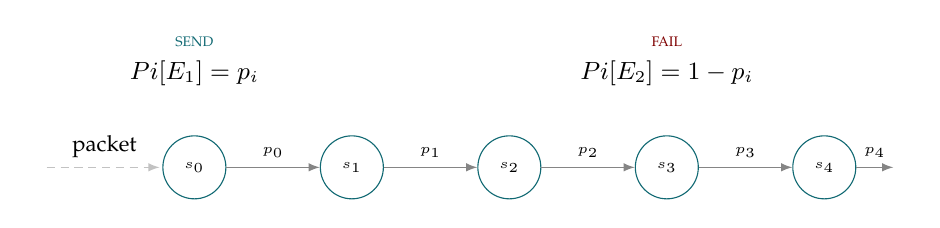
\begin{tikzpicture}[
    serviceNode/.style={circle,draw=customDarkBlue,fill=white,thick,inner sep=0pt,minimum size=8mm, thin},
    output/.style={circle,draw=black,fill=customGreen,thick,inner sep=0pt,minimum size=8mm},
    hidden/.style={circle,draw=black,fill=customRed,thick,inner sep=0pt,minimum size=8mm},
    function/.style={rectangle,draw=black,fill=customGrey,thick,inner sep=0pt,minimum size=8mm},
    post/.style={thin, -latex, color=customGrey},
    inEdge/.style={-latex,shorten >=1pt, thin,color=customGrey!50}
    ]
		% output invisible node
		\node[draw=none] (pOut) at (9, 3) {};
		
		\node[serviceNode] (s4) at (8, 3) {\tiny $s_4$}
		edge [post] node[auto] {\textcolor{black}{\tiny $p_4$}} (pOut);
		
		\node[serviceNode, label={[label distance=0.5cm,align=center,font=\fontsize{12}{12}\selectfont]\textcolor{customDarkRed}{\tiny FAIL}\\\small $Pi[E_2]=1 - p_i$}] (s3) at (6, 3) {\tiny $s_3$}
		edge [post] node[auto] {\textcolor{black}{\tiny $p_3$}} (s4);
		
		\node[serviceNode] (s2) at (4, 3) {\tiny $s_2$}
		edge [post] node[auto] {\textcolor{black}{\tiny $p_2$}} (s3);
		
		\node[serviceNode] (s1) at (2, 3) {\tiny $s_1$}
		edge [post] node[auto] {\textcolor{black}{\tiny $p_1$}} (s2);
		
		\node[serviceNode,label={[label distance=0.5cm,align=center,font=\fontsize{12}{12}\selectfont]\textcolor{customDarkBlue}{\tiny SEND}\\\small $Pi[E_1]=p_i$}] (s0) at (0, 3){\tiny $s_0$}
		edge [post] node[auto] {\textcolor{black}{\tiny $p_0$}} (s1);
		
		% input invisible node
		\node[draw=none] (p0) at (-2, 3) {}
		edge [inEdge, densely dashed] node[auto] {\textcolor{black}{\footnotesize packet}}  (s0);
\end{tikzpicture}
	\caption{An example of a simulation configuration with $5$ services, where each service has its own probability distribution of events $Pr_i$}.
	\label{figure:simulation}
\end{figure}

The simulation generates a log file with log messages printed out by the services. Below we see some sample log message entries in the simulated log file. The packets are sent sequentially between the services in ascending order. If service $i$ cannot send the packet to the next service, it logs a message \texttt{No packet was sent} and the packet does not reach another service $j$ such that $j$ >$i$. These services also do not record a log message. 

\begin{verbatim}
========== Starting new simulation ==========
Epoch: 0 Service 0: Successfully sent a packet
Epoch: 0 Service 1: Successfully sent a packet
Epoch: 0 Service 2: Successfully sent a packet
Epoch: 0 Service 3: Successfully sent a packet
Epoch: 0 Service 4: Successfully sent a packet
Epoch: 1 Service 0: Successfully sent a packet
Epoch: 1 Service 1: Successfully sent a packet
Epoch: 1 Service 2: No packet was sent
Epoch: 2 Service 0: Successfully sent a packet
Epoch: 2 Service 1: Successfully sent a packet
Epoch: 2 Service 2: Successfully sent a packet
Epoch: 2 Service 3: Successfully sent a packet
Epoch: 2 Service 4: Successfully sent a packet
Epoch: 3 Service 0: Successfully sent a packet
Epoch: 3 Service 1: Successfully sent a packet
Epoch: 3 Service 2: Successfully sent a packet
Epoch: 3 Service 3: Successfully sent a packet
Epoch: 3 Service 4: Successfully sent a packet
Epoch: 4 Service 0: Successfully sent a packet
Epoch: 4 Service 1: Successfully sent a packet
Epoch: 4 Service 2: Successfully sent a packet
Epoch: 4 Service 3: Successfully sent a packet
Epoch: 4 Service 4: Successfully sent a packet
Epoch: 5 Service 0: Successfully sent a packet
Epoch: 5 Service 1: Successfully sent a packet
Epoch: 5 Service 2: Successfully sent a packet
Epoch: 5 Service 3: Successfully sent a packet
Epoch: 5 Service 4: Successfully sent a packet
Epoch: 6 Service 0: Successfully sent a packet
Epoch: 6 Service 1: Successfully sent a packet
Epoch: 6 Service 2: No packet was sent
 \end{verbatim}
 
We can convert the set of log messages into a vector embedding, as seen in Table \ref{tab:simulation}. Each row represents an epoch and each cell contains an output of the simulation of a corresponding service, where $1$ corresponds to event $E_1$ and $0$ corresponds to event $E_2$. Figure \ref{fig:simulationPlot} shows the number of services that successfully received and sent a packet for each epoch. As expected from the probability distribution of events, it can be seen that the majority of epochs for all $5$ services completed successfully. The service numbered $2$ was assigned a higher probability of failure, corresponding to the number $2$ of successfully completed services on the y-axis. 

\begin{table}[!h]
\centering
\begin{tabular}{@{}p{1.5cm}p{1.5cm}p{1.5cm}p{1.5cm}p{1.5cm}p{1.5cm}@{}}
\toprule
Epoch      & $\mathbf{s_0}$ & $\mathbf{s_1}$ & $\mathbf{s_2}$ & $\mathbf{s_3}$ & $\mathbf{s_4}$ \\ \toprule
\textbf{0} & 1             & 1             & 1             & 1             & 1             \\
\textbf{1} & 1             & 1             & 0             & 0             & 0             \\
\textbf{2} & 1             & 1             & 1             & 1             & 1             \\
\textbf{3} & 1             & 1             & 1             & 1             & 1             \\
\textbf{4}          & 1             & 1             & 1             & 1             & 1             \\
\textbf{5}          & 1             & 1             & 1             & 1             & 1             \\
\textbf{6}          & 1             & 1             & 1             & 1             & 1             \\ \bottomrule
\end{tabular}
\caption{An example of numerical embedding obtained from the first $7$ epochs of the simulation of the toy example.}\label{tab:simulation}
\end{table}

\begin{figure}[!h]
        \centerline{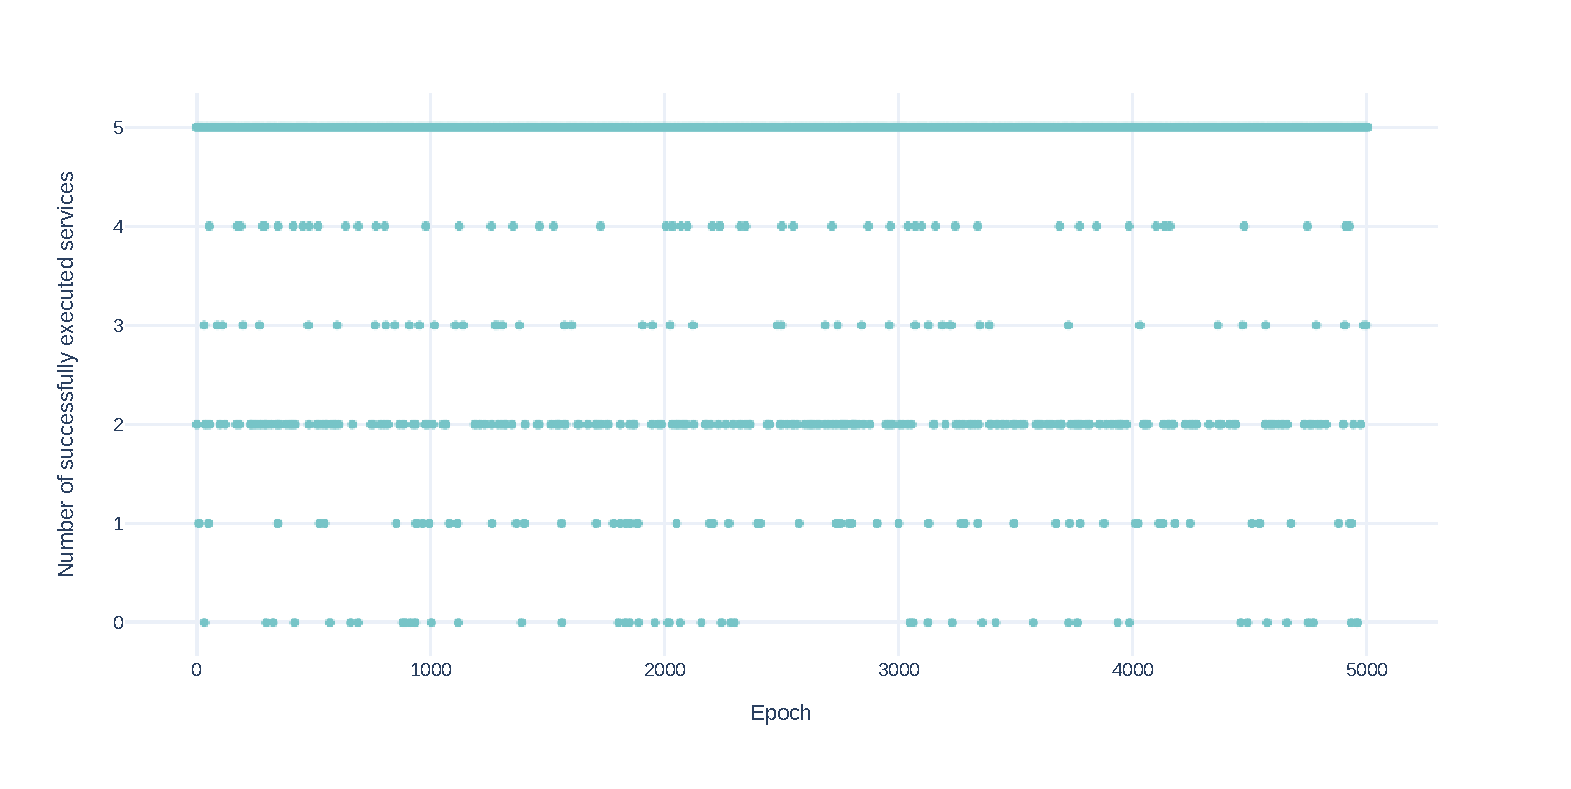
\includegraphics[scale=.5]{img/dummy_data_plot.pdf}}
        \caption{The result of running our simulation for $5000$ epochs.}
        \label{fig:simulationPlot}
\end{figure}

The obtained simulated dataset can be easily modified to generate labels. If a line contains only ones, the assigned label is \texttt{no\_service}. If a line contains a zero, its label is the index of the first service that failed to send a packet. This embedding is then used as input to build a logistic regression and random forest model. The toy example is intended to provide a better understanding of how an unstructured text input can be converted into a format suitable for machine learning algorithms.

\section{Data Collection}
\label{data_collection}
By data collection, we mean the process of collecting log data from the observed system in such a way that the logs can be further parsed, processed, and fed to the machine learning model.

The system we studied follows the microservices architecture pattern as described in Section~\ref{smart-connect:architecture} on the architecture of SmartConnect.\\

\subsection{Logging}

Traditionally, an application performs logging by sending messages to
(pseudo) files \texttt{stderr} (standard error) and \texttt{stdout} (standard output). It can be combined with appending these logs also to a dedicated file with \texttt{.log} extension. Both methods are typically used by services running as containerized applications in Pods\footnote{\url{https://kubernetes.io/docs/concepts/cluster-administration/logging/}}.

In microservices architecture, this method of logging may not be sufficient because an MSA system usually consists of many applications and the logs are scattered in many places. In addition, the individual services are often replaced and the contents of the log files are subsequently removed.

In addition, for systems that produce a large amount of logs, persisting the logs to files and storing them in the service Pod's file system can cause the node's storage space to be overused. For this reason, services such as logrotate\footnote{\url{https://linux.die.net/man/8/logrotate}} are used. Logrotate collects logs, sends them to another location where they can be persisted without affecting the performance of the MSA system, and removes them from the Pod's node. On the other hand, this means that when a Pod is checked, only the most recent (if any) logs can be found in the Pod's \texttt{log} file.

SmartConnect MSA takes a similar approach to logrotate.

Filebeat\footnote{\url{https://www.elastic.co/guide/en/beats/filebeat/7.10/filebeat-overview.html}} from ELK (Elasticsearch, Logstash, Kibana)\footnote{\url{https://www.elastic.co/what-is/elk-stack}} is used to pass the data collected by the system's Pods to the Elasticsearch engine (introduced in Section~\ref{smart-connect:elastic-search}). 
The engine provides an authority for storing logs of the system and is considered as the single source of truth since the log data is persisted there.

\subsection{Implementation}

In summary, the following options are available for log collection in the SmartConnect system:
\begin{enumerate}
\item Saving the output of the command \texttt{kubectl logs \$\{POD\}} for each relevant Pod 
\item Collecting the data stored in \texttt{\$\{POD\}:/var/log/*.log} for each Pod \item Requesting logs from the Elasticsearch server from SmartConnect
\end{enumerate}


To gauge the possibilities, the first two items represent the same idea, just executed in a different way - the \texttt{logs} command simply prints the output of the desired \texttt{.log} file to \texttt{stdout}. 
It is very easy to get the logs of a single Pod, but to gather all the desired information about the whole system, all microservices need to be crawled individually. Moreover, as mentioned earlier, the main drawback of these approaches is that only logs that have not yet been fetched by filebeat are accessible.

Therefore, in order to collect log data from several hours of system operation, services would need to be queried relatively frequently. These methods also introduce complexity into the post-processing of the data once collected, as we cannot guarantee the uniqueness of the entries in these approaches.

On the other hand, the third option is more difficult to automate, but promises a more structured way to obtain the logs. Moreover, given the features of Elasticsearch, it should also provide a faster solution for data collection.

In Motorola, developers review logs stored in their Elasticsearch engine via the Kibana web user interface. The UI makes it easy to visualize and filter log data, but on the down side, its export options are not well suited for a structured way of downloading the data. Regardless of these limitations, a size limit needs to be set for the exports. The limit should not be much larger than the default 10 MB, as it can potentially have a negative impact on the performance\footnote{\url{https://www.elastic.co/guide/en/kibana/current/reporting-settings-kb.html}}. Based on our requirements, 10 MB of log data would not cover more than a few minutes of logs.

Another option, using ELK stack, would be to make use of the REST APIs of Elasticsearch\footnote{\url{https://www.elastic.co/guide/en/elasticsearch/reference/current/rest-apis.html}}. However, for security reasons, some companies choose not to expose this API to the Internet - Motorola is one of them.
So the only way to access the application programming interface is to make the calls from within the cluster.

We deployed a service called \texttt{elk-query-service} within the cluster that handles search queries to the Elasticsearch. Our service provides minimalistic functionality that can be accessed within the company.
\texttt{\justify elk-query-service} can be invoked with two date arguments indicating the start and end of the time window. Logs between the start and end dates are downloaded to the \texttt{elk-query-service} Pod and can be transferred to the node, where they can be further used in a machine learning anomaly detection pipeline, as proposed in Section~\ref{future:pipeline} for future work. The high-level architecture of our data collection solution is schematically shown in Figure~\ref{fig:data_collection_elastic}.

\begin{figure}[!tbp] \centering {
   \begin{tikzpicture} [
    edge/.style={-latex,shorten >=1pt, thin, color=customGrey},
    line/.style={-,shorten >=1pt, thin, color=customGrey},
    mainRectangle/.style={rectangle, draw=customBlue, align=left},
]

\node[inner sep=0pt] (mlHost) at (-2,0) {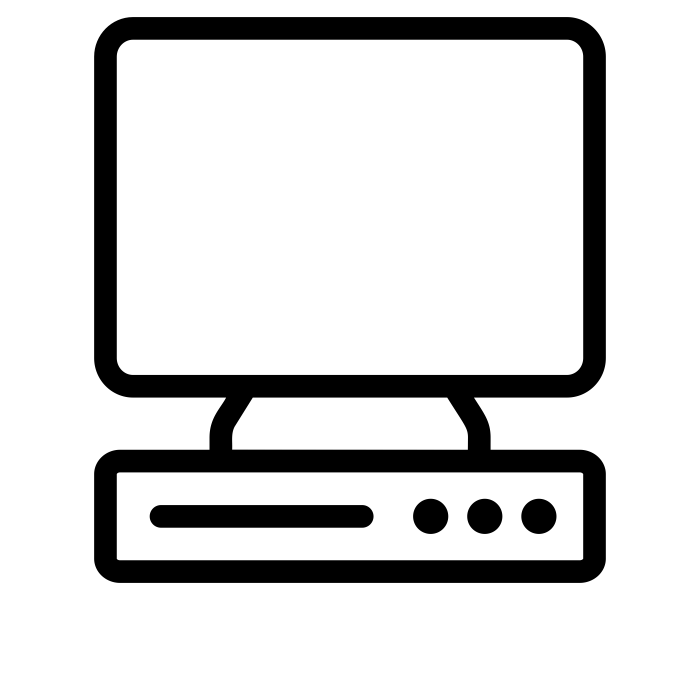
\includegraphics[width=.12\textwidth]{img/computer-icon.png}};
\node[align=center,anchor=north] (lab) at (mlHost.south) {\footnotesize Machine Learning\\\footnotesize Host};
    
\node[mainRectangle, minimum width={20mm}, label={[label distance=2mm]below: \footnotesize MSI Kubernetes Cluster}] (kubernetesCluster) at (4, 0) {
    \begin{tikzpicture}[node distance=1cm,outer sep=0pt, align=left]
        \node[inner sep=0pt, label={[label distance=2mm]below:\footnotesize elk-query-service}] (pod1) at (-2,0)
        {
\includegraphics[width=.08\textwidth]{img/pod.png}};   
        
        \node[inner sep=0pt, label={[label distance=2mm]below:\footnotesize elastic-search}] (pod2) at (2,0)
    {
\includegraphics[width=.08\textwidth]{img/pod.png}};
    
        \node[draw=none] (a) at (-2.5, 0) {};
        \node[draw=none] (b) at (2.5, 0) {};
        \draw [edge] (a) -- node[anchor=south] {\tiny \textcolor{customDarkRed}{Search Query}} (b);
        \node[draw=none] (c) at (-2.5, -0.3) {};
        \node[draw=none] (d) at (2.5, -0.3) {};
        \draw [edge] (d) -- node[anchor=south] [label=below:\tiny \textcolor{customDarkRed}{Response}]{} (c);
        
        \node[mainRectangle, minimum width={10mm}, label={[label distance=2mm]below: \footnotesize Observed System}] (system) at (0, -3.5) {
            \begin{tikzpicture}[node distance=1cm,outer sep=0pt, align=left]
                \node[inner sep=0pt] (pod3) at (2,0)
                {
\includegraphics[width=.06\textwidth]{img/pod.png}};
                \node[inner sep=0pt] (pod4) at (2.8,0)
                {
\includegraphics[width=.06\textwidth]{img/pod.png}};
                \node[inner sep=0pt] (pod5) at (3.6,0)
                {
\includegraphics[width=.06\textwidth]{img/pod.png}};
                \node[draw=none] (dots) at (4.2, 0) {...};
                \node[inner sep=0pt] (pod3) at (4.8,0)
                {
\includegraphics[width=.06\textwidth]{img/pod.png}};
                \node[inner sep=0pt] (pod4) at (5.6,0)
                {
\includegraphics[width=.06\textwidth]{img/pod.png}};
                \node[inner sep=0pt] (pod5) at (6.4,0)
                {
\includegraphics[width=.06\textwidth]{img/pod.png}};
            \end{tikzpicture} 
        };
        
        \node[draw=none] (es) at (2.2, -1.2) {};
        \node[draw=none] (p1) at (-2.5, -3.3) {};
        \draw [edge] (p1) -- node[anchor=south] {} (es);
        
        \node[draw=none] (p2) at (-1.7, -3.3) {};
        \draw [edge] (p2) -- node[anchor=south] {} (es);
        
        \node[draw=none] (p3) at (-0.9, -3.3) {};
        \draw [edge] (p3) -- node[anchor=south] {} (es);
        
        \node[draw=none] (p4) at (0.4, -3.3) {};
        \draw [edge] (p4) -- node[anchor=south] {} (es);
        
        \node[draw=none] (p5) at (1.3, -3.3) {};
        \draw [edge] (p5) -- node[anchor=south] {} (es);
        
        \node[draw=none] (p6) at (2.15, -3.3) {};
        \draw [edge] (p6) -- node[anchor=south] {} (es);
     
    \end{tikzpicture} 
};
    
    \node[draw=none] (eqs) at (1.6, 2) {};
    \node[draw=none] (mlHostStart1) at (-1.3, 0.8) {};
    \node[draw=none] (mlHostStart2) at (-1.3, 0.5) {};
    \draw [edge] (mlHostStart1) -- node[anchor=south, rotate=22] {\tiny \textcolor{customDarkRed}{Start Date, End Date}} (eqs);
    
    \node[draw=none] (eqs2) at (1.6, 1.7) {};
    \draw [edge] (eqs2) -- node[anchor=north, rotate=22] {\tiny \textcolor{customDarkRed}{Logs}} (mlHostStart2);

\end{tikzpicture}
   \caption{The implemented solution for collecting log data. Node with access rights to the Kubernetes cluster calls an orchestration script with two arguments - start date and end date. \texttt{elk-query-service} downloads the desired logs that match the date specification. The script stores the response on the machine learning node, which can proceed to the next step - training and evaluating ML models.}
	\label{fig:data_collection_elastic}
	}
\end{figure}

\newpage

\section{Log Parsing}
This section describes our technique for parsing the raw and unstructured logs obtained from the analyzed system.

As stated in Section~\ref{log_parsing_techniques}, there are many different basic approaches to what techniques should be used when extracting message templates from logs. 
Therefore, we have developed an additional abstraction layer on top of the actual parser that makes our solution less dependent on which specific template mining algorithm is used.

The experiments therefore work with an object \texttt{LogCategorizer} that exposes the functionality to clients. To name a few of the \texttt{LogCategorizer} methods, it provides the following, among others:

\begin{itemize}
    \item \texttt{process\textunderscore log\textunderscore message(self, log\textunderscore message: str)\\ -> LogCategory}
    \item \texttt{process\textunderscore log\textunderscore messages(self, log\textunderscore messages: List[str])\\ -> List[LogCategory]}
    \item \texttt{process\textunderscore file(self, input\textunderscore file\textunderscore name: str)}
\end{itemize}

The actual reading and creation of templates by these methods is done by an instance of \texttt{LogParser}. \texttt{LogParser} is an abstraction - an interface used by \texttt{LogCategorizer}. Any implementation of the parser must satisfy this contract defined by the interface. The interface defines only the bare minimum of functionality required by a meaningful log template miner, and that is a pair of methods:
\begin{itemize}
    \item \texttt{get\textunderscore all\textunderscore templates(self) -> List[str]}
    \item \texttt{process\textunderscore log\textunderscore message(self, log\textunderscore message: str) -> str}
\end{itemize}
Therefore, an implementation of a log parser should be able to return all templates it has identified up to the call to the \texttt{get\textunderscore all\textunderscore templates} method. The other method returns a template based on the raw log message entered.\\

Our implementation follows the adapter design pattern \cite{gamma1995design_pattern_adapter}, since the goal is to convert interfaces of specific log parsing libraries that may differ drastically in terms of the API they expose.

This allows us to decouple the implementation of the algorithm that identifies templates from logs from our overall goal and opens the way for easy comparison with different template mining strategies.\\

 \begin{figure}[!h] \centering {
   \resizebox{\textwidth}{!}{
\begin{tikzpicture}

\tikzumlset{draw=customBlue, fill class=white, }

edge/.style={color=black}

\umlclass[x=-9, y=0, width=5ex, name=logCategorizer, text=customDarkRed]{LogCategorizer}{}{
\textcolor{black}{\footnotesize+ try\_insert\_new\_template(template: str)}\\
\footnotesize{+ get\_all\_templates(): [(int, str)]} \\
\footnotesize{+ process\_log\_message(log\_message: str): LogCategory}\\
\footnotesize{+ process\_log\_messages(log\_messages: [str]): [LogCategory]}\\
\footnotesize{+ process\_file(file\_name: str): [LogCategory]}}

\umlclass[x=-9, y=-4, width=5ex, name=logCategory, text=customDarkRed]{LogCategory}{
\textcolor{black}{\footnotesize{+ category\_id: int}}\\
\footnotesize{+ template: str}}{}

\umlclass[x=0, y=0, name=logParser, text=customDarkRed, type=interface]{LogParser}{}{
\textcolor{black}{\footnotesize{+ get\_all\_templates(): [str]}}\\
\footnotesize{+ process\_log\_message(log\_message: str): str}}

\umlclass[x=0, y=-4, name=drain3Parser, text=customDarkRed]{Drain3Parser}{
\textcolor{black}{\footnotesize{- template\_miner: TemplateMiner}}}
{
\textcolor{black}{\footnotesize{+ get\_all\_templates(): [str]}}\\
\footnotesize{+ process\_log\_message(log\_message: str): str}
}

\umlclass[x=0, y=-8, name=templateMiner, text=customDarkRed]{TemplateMiner}
{
\textcolor{black}{\footnotesize{+ clusters}}\\
\footnotesize{+ persistence}}
{
\textcolor{black}{\footnotesize{+ add\_log\_message(log\_message: str)}}
}

\umluniassoc [color=customGrey] {LogCategorizer}{LogCategory}
\umluniassoc [color=customGrey] {LogCategorizer}{LogParser}
\umluniassoc [color=customGrey] {Drain3Parser}{TemplateMiner}
\umldep [color=customGrey] {Drain3Parser}{LogParser}

\end{tikzpicture}
}
   \caption{Architecture for parsing classes. Application of the adapter design pattern: \texttt{LogParser} as adapter, \texttt{Drain3Parser} takes role of concrete adaptee, \texttt{TemplateMiner} is adaptee - class defined in other framework with incompatible interface and needs to be converted.}
	\label{fig:uml_parsers}
	}
\end{figure}

In Section~\ref{parser_summary} we mention that our decision was to proceed with the framework Drain \cite{drain2017}, which performs online fixed-depth tree template mining. The current implementation of the algorithm we use is \texttt{Drain3} by IBM\footnote{\url{https://github.com/ IBM /Drain3}}. The algorithm follows a template of 5 steps as described in more detail in Section~\ref{fixed_depth_tree}:
\begin{enumerate}
    \item Preprocess by Domain Knowledge
    \item Search by Log Message Length
    \item Search by Preceding Tokens
    \item Search by Token Similarity
    \item Update the Parse Tree
\end{enumerate}

Let's pay more attention to the first step. It provides us, the users, with the option to input encoded assumptions and knowledge about the logs that are produced by the system.
It is quite intuitive to assume that this domain knowledge, if properly inserted, should improve the performance and precision of mining algorithms. An empirical study \cite{he2016} confirms this conjecture.
However, we argue that this algorithm tuning technique may not be the right choice in all use cases. With our solution, we attempt to analyze a system that is highly fluid and therefore likely to change over time. This, coupled with the fact that many developers from multiple teams and companies (taking into account also external software on which the software system depends), it is not feasible to obtain a single source of truth regarding domain knowledge related to logging. Conversely, we aim for a solution that can learn and adapt to changes as independently as possible.\\

This goal of adaptability is also reflected in the fact that we ultimately decided to use an online parser.
To recall a definition of an online template miner from Section~\ref{log_template_mining}, an online template miner is such a parser that does not need to see the entire dataset to start analyzing message templates. It can perform categorization on the fly while simultaneously updating its internal state, which stores acquired knowledge about the domain.\\
Drain provides the ability to persist this internal state between multiple runs, giving us the best of both worlds - the parser learns the patterns occurring in the logs over time to improve, while being able to respond to new data in a flexible way.

We did not change steps 2. - 4. as the default parameters \cite{ibmdrain3} produced results that extracted correct templates from the observed logs.

For the last step, updating the parse tree, the Drain3 implementation provides the option to persist the state of the parse tree in the JSON file format. This allows us to reuse the domain knowledge acquired by the template miner across restarts of our solution.
This is an extremely useful feature, since we can assume that all logs come from the same system, we can reuse the parse tree already built in previous runs and enrich it.
Drain3 provides several ways to save the snapshot of the parse tree, we use the one that saves the state to a file.

\section{Feature Engineering}
\label{section:featureEngineering}
Now that we have obtained unique event types from the unstructured log messages, we need to select valuable variables, group them, and encode them into a numeric form that can be further used by machine learning algorithms. This process is called \textit{feature engineering} or \textit{feature extraction}. Feature extraction is the process of generating new features through transformations of the original feature set. In our thesis, we also refer to the generated features as \textit{embeddings}.

The feature engineering step is crucial. The embeddings should be able to summarize valuable information and complex relationships in the dataset, which directly affects the performance of the learning model and the speed of training, and avoids overfitting. The log event types generated in the previous step are used as input to the feature engineering step. The output is a numerical matrix. 

\subsection{Windowing}
% https://core.ac.uk/download/pdf/196555557.pdf page 22

In time series anomaly detection, a common concept applied in feature extraction is \textit{windowing}. 
Logs are grouped into smaller blocks called \textit{windows}, where each window represents a sequence of logs. In some previous approaches \cite{xu2009}, windowing was applied by grouping events by the same session identifier, so that each window represents a job execution with a unique identifier. This solution is not applicable in our case because we do not have a session or process identifier in our raw dataset.

Log data is also non-uniformly distributed time series data, since there is naturally a time of occurrence of each log. Therefore, another intuitive and commonly used approach to windowing is to generate a set of subsequences of time series. For example, suppose we have log lines ordered by timestamp and the length of the time window is $q$. Then, log line number $1$ to log line number $q$ is enclosed in the same time window $1$ and encoded as the first row of the resulting feature matrix. The goal of the next step of anomaly detection is to say for each subsequence whether it contains an anomaly or not. In our work, we use a timestamp based windowing, which is also described in the next part of the text.

A set of time series subsequences can be generated using \textbf{sliding windows}. Consider a time series $\mathbf{x} = x_1, x_2, ..., x_n$ of length $n$. We want to extract subsequences $\mathbf{x_i}$ of length $m$. In other words, we want to apply sliding windows of length $m$ and move over the time series until we reach the end of the data set. At each move, we shift the window $r$ time steps to the right. As a result, we get $p$ windows, where $p$ is defined as
    \begin{gather*}
        p = \dfrac{n - m}{r} + 1
    \end{gather*}

and the generated windows are of the form 

\begin{gather*}
    \mathbf{x_1} = x_{11}, x_{12},..., x_{1m} \\
    \mathbf{x_2} = x_{21}, x_{22},..., x_{2m} \\
    \ldots\\
    \mathbf{x_p} = x_{p1}, x_{p2},..., x_{pm} 
\end{gather*}

The size of the step $r$ is a very important parameter. If one chooses $r$ very small, e.g. $r = 1$, such that the subsequences are obtained by sliding the window one step at a time, one has the advantage that no anomalous sequence can be missed in this approach. However, considering the large dataset that grows with time, computing such partial sequences is inefficient and time consuming. On the contrary, we can choose a high value of $r$. For example, if we set $r$ to the length of the sliding window $m$ ($r = m$), then there is no overlap between the windows. The advantage of fewer generated subsequences and less processing time comes with a greater risk of missing anomalous subsequences. 

Another parameter to consider is the size of the sliding window $m$. The ideal size really depends on the application domain and how many consecutive log entries on average can represent an anomaly. 

Thus, setting the size of the step parameter $r$ and the length of the sliding window $m$ is a tradeoff between accuracy and processing time. A useful rule is to choose the value of $r$ proportional to the length of the subsequences \cite{izakian2013}. Consequently, longer subsequences have a higher value of $r$, while shorter subsequences have a lower value of $r$. The number of log lines contained in each window may vary. 

In our work, instead of considering the number of log lines in each window, we consider the size of a subsequence in terms of a time span.

\begin{figure}[!tbp] \centering {
	\begin{subfigure}[b]{1\textwidth}
        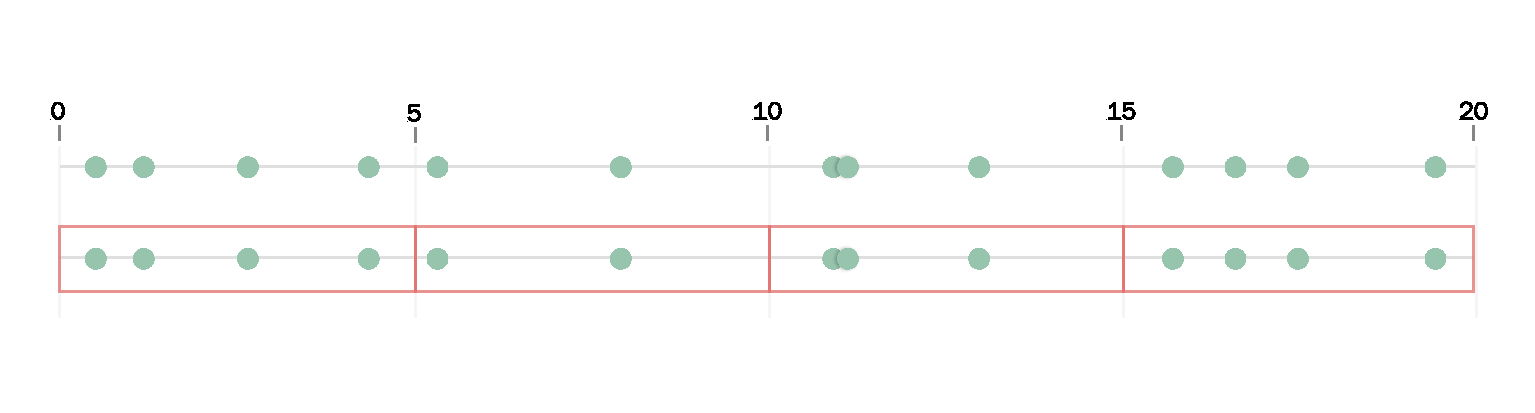
\includegraphics[width=\textwidth]{img/windowing.pdf}		    \caption{Sliding window with a fixed length of $m = 5$ and step size $r = m = 5$}
		\label{fig:f1}
	\end{subfigure} \\
	\hfill
		
    \begin{subfigure}[b]{1\textwidth}
   	    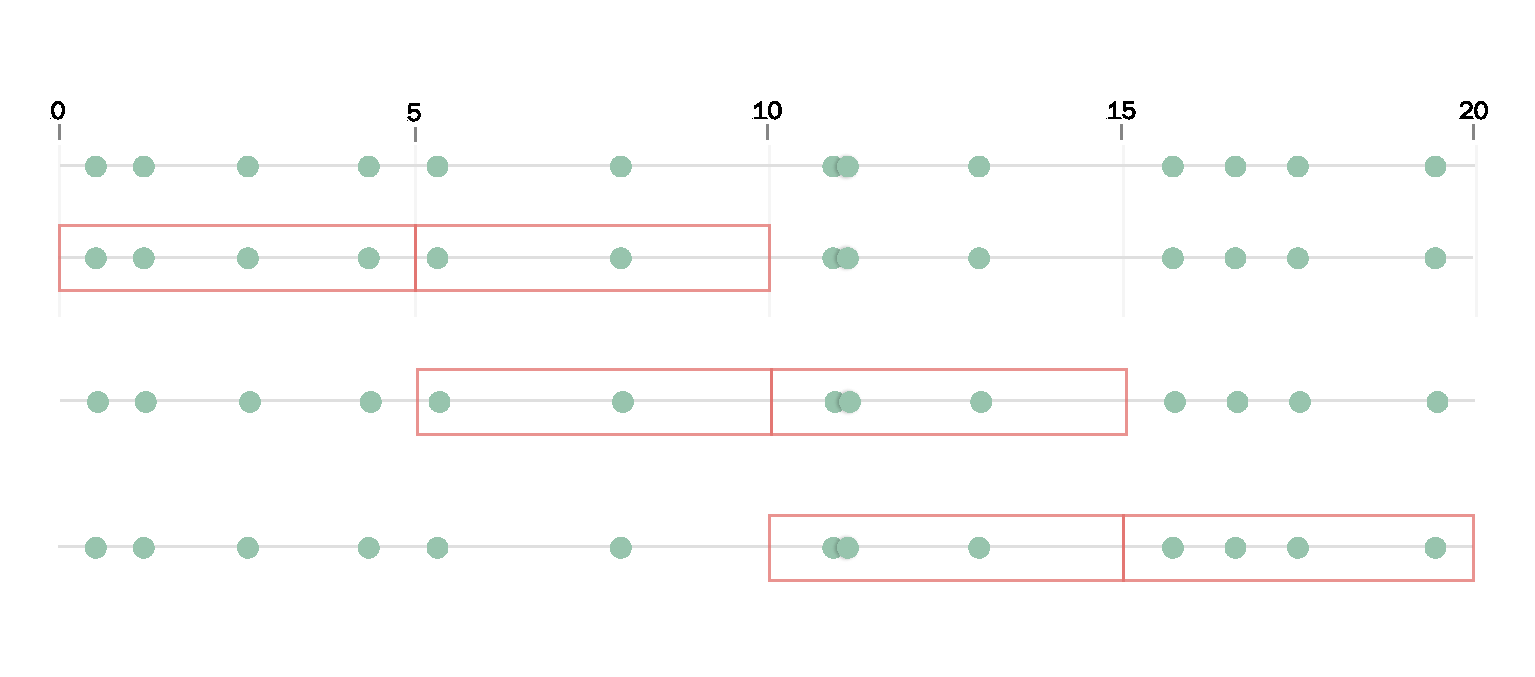
\includegraphics[width=\textwidth]{img/windowing-2.pdf}
		\caption{Sliding window with a fixed length of $m = 10$ and step size $r = 5$}
	\end{subfigure}
	
	\caption{Two types of windowing with different step size $r$. (a) shows sliding windows created without overlap. (b) illustrates sliding windows created by a step size of half the window size, resulting in overlap between subsequent windows.}
	\label{fig:windowing}
	}
\end{figure}

\subsection{Feature embedding}
\label{subsection:features}
After applying the sliding window to generate log sequences, the final step of feature extraction is to construct the feature matrix that can be passed as input to the ML algorithms. In our thesis, we experiment with two different types of embeddings, where both representations describe a set of logs in log sequences: \textit{event count matrix} and \textit{TF-IDF weighted matrix}. Figure \ref{fig:feature-extraction} shows an example of the process of generating a single log sequence into a feature matrix. We assume that logs in sequences are highly correlated. To help the reader understand the differences between the two proposed embeddings, we provide a summary in Table \ref{tab:embeddings-summary}.

\begin{figure}[!h] \centering {
   \begin{tikzpicture} [
    edge/.style={-latex,shorten >=1pt, thin, color=customGrey},
    line/.style={-,shorten >=1pt, thin, color=customGrey},
    mainRectangle/.style={rectangle, draw=customBlue, align=left}
]

    % RAW LOG MESSAGE SEQUENCE
    \node[mainRectangle, minimum width={110mm}, label={[label distance=2mm, align=center] { \footnotesize Raw log message sequence}}] (logSequence) at (0, 0) {
        \begin{tikzpicture}[node distance=1cm,outer sep=0pt, align=left]
            \node[draw=none] (log1) at (0, 0) {\tiny 1 \textcolor{customDarkBlue}{2020-10-04 19:15:00} Error in estabilishing TLS connection: ip: {52,240,151,125}, port: 17857\\
            \tiny 2 \textcolor{customDarkBlue}{2020-10-04 19:15:07} Start call: Service.start()\\
            \tiny 3 \textcolor{customDarkBlue}{2020-10-04 19:20:01} Received message: \#PID<0.2108.0> type: DELETED rv: 55000\\
            \tiny 4 \textcolor{customDarkBlue}{2020-10-04 19:15:07} New TLS connection attempt client\_ip: \{13,65,95,152\}, port: 26097\\
            \tiny 5 \textcolor{customDarkBlue}{2020-10-04 19:15:07} Received message: \#PID<0.2108.0> type: MODIFIED rv: 55000};
        \end{tikzpicture} 
    };
    
    % EVENT TEMPLATES
    \node[mainRectangle, minimum width={90mm}, label={[label distance=2mm] { \footnotesize Event templates}}] (eventTemplates) at (0, -5) {
        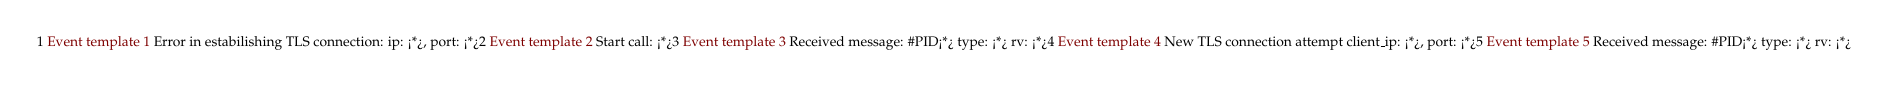
\begin{tikzpicture}[node distance=1cm,outer sep=0pt]
            \node[draw=none] (templates) at (-2, 0) {
            \tiny 1 \textcolor{customDarkRed}{Event template 1} Error in estabilishing TLS connection: ip: <*>, port: <*>\\
            \tiny 2 \textcolor{customDarkRed}{Event template 2} Start call: <*>\\
            \tiny 3 \textcolor{customDarkRed}{Event template 3} Received message: \#PID<*> type: <*> rv: <*>\\
            \tiny 4 \textcolor{customDarkRed}{Event template 4} New TLS connection attempt client\_ip: <*>, port: <*>\\
            \tiny 5 \textcolor{customDarkRed}{Event template 5} Received message: \#PID<*> type: <*> rv: <*>};
        \end{tikzpicture} 
    };
    
    \draw[edge] (logSequence) -- (0, -3.1) node [midway, fill=white] {\footnotesize \textcolor{customGreen}{log parsing}};
    
     % EVENT TEMPLATES
    \node[mainRectangle, label={[label distance=2mm] { \footnotesize Feature vectors}}] (featureVectors) at (0, -9.5) {
        \begin{tikzpicture}[node distance=1cm,outer sep=0pt]
             % ML METHODS
            \node[mainRectangle, align=center, densely dashed, minimum width={15mm}, label={[label distance=0mm, align=center]{\scriptsize Event count vector}}] (eventCountVector) at (-1, -9.5) {
                \begin{tikzpicture}[
                    cell/.style={draw, minimum width={4mm}, minimum height={4mm}, solid, thin}
                ]
                \matrix [nodes=draw] 
                {
                \node [cell] {\tiny 1}; & \node [cell] {\tiny 1};   & \node [cell] {\tiny 2}; & \node [cell] {\tiny 1}; & \node[cell]  {\tiny 0};  & \node[cell]  {\tiny 0}; & \node [cell] {\tiny 0}; & \node [cell] {\tiny 0};\\
            };
                \end{tikzpicture} 
            };
            
            \node[mainRectangle, align=center, densely dashed, minimum width={15mm}, label={[label distance=0mm, align=center]{\scriptsize TF-IDF vector}}] (tfIdfVector) at (4, -9.5) {
                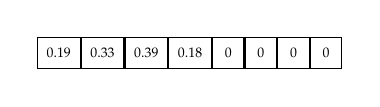
\begin{tikzpicture} [
                    cell/.style={draw, minimum width={4mm}, minimum height={4mm}, solid, thin}
                ]
                \matrix [nodes=draw]
                {
                \node [cell] {\tiny 0.19}; & \node [cell] {\tiny 0.33};   & \node [cell] {\tiny 0.39}; & \node [cell] {\tiny 0.18}; & \node[cell]  {\tiny 0};  & \node[cell]  {\tiny 0}; & \node [cell] {\tiny 0}; & \node [cell] {\tiny 0};\\
            };
                \end{tikzpicture} 
            };
        \end{tikzpicture} 
    };
    
    \draw[edge] (eventTemplates) -- (0, -8) node [midway, fill=white] {\footnotesize \textcolor{customGreen}{feature extraction}};
    

\end{tikzpicture}
   \caption{An example of encoding log sequence into two types of feature vectors: \textit{Event count vector} and \textit{TF-IDF vector}. We assume that there is $8$ event templates in the collection, thus the output vectors are also of length $8$.}
	\label{fig:feature-extraction}
	}
\end{figure}

\begin{table}
\centering
\resizebox{\textwidth}{!}{\begin{tabular}{@{}ccc@{}}
\toprule
\textbf{Matrix type} & \textbf{Row}               & \textbf{Column}                                          \\ \midrule
\textbf{\textcolor{customRed}{Event count}}    & log sequence & Frequency of event type in the log sequence              \\
\textbf{\textcolor{customRed}{TF-IDF}}         & log sequence & IDF weighted frequency of event type in the log sequence \\ \bottomrule
\end{tabular}}
\caption{A summary of feature matrix types using in our thesis }\label{tab:embeddings-summary}
\end{table}

\subsubsection*{Event Count Matrix}
A simple approach to obtain such a representation is to create an event count vector for each log sequence. In other words, for each log sequence, we count the number of event type identifiers and store it as a row vector of an event count matrix. The length of the vector corresponds to the number of unique event types detected in the log parsing section, and each component of the vector corresponds to an event type. The value at each position in the vector is the frequency of the event types. For event types that did not occur in the log sequence, the value is zero. Thus, one row of the event count matrix represents a single log sequence. The valuable information that contributes to the machine learning model behind the event count matrix is determining what a normal number of events is and what it means to deviate from the normal counts.

%http://essay.utwente.nl/83142/1/Ma_MA_FacultyOfEEMathematicsAndCS.pdf illustration

This way of constructing the event count matrix is known in the literature as a natural language processing (NLP) model for feature extraction called \textit{Bag-of-Words} (BoW) \cite{informationRetrieval2008}. BoW treats each log sequence as a \textit{document} and for each \textit{word} (in our case, a word is an event type) in a document, a \textit{weight} is assigned. The weight depends on the number of occurrences of the term in the document. The length of the vector is equal to the number of unique words in the database (analogous to all parsed event types). The weight score is then called \textit{Term Frequency} (TF) and denoted by $tf_{t,d}$, where subscript $t$ refers to the term (event type) and $d$ refers to the document (log sequence) and $f_{t,d}$ is a frequency of term $t$ in document $d$. The term frequency describes the importance of an event type in a log sequence.

\begin{gather}
    tf_{t,d} = \dfrac{f_{t,d}}{\sum_{t'}f_{t', d}}
\end{gather}

In other words, $tf_{t, d}$ is the probability of $t$ occurring in $d$.

\subsubsection*{TF-IDF}
Another weighting scheme widely used in Information Retrieval is called \textit{term frequency–inverse document frequency} (TF-IDF). 

If we use only the standard term frequency, we have to deal with an important issue. After defining the term frequency, all event types are considered equally important \cite{informationRetrieval2008}. However, we also want to know how important a term is not only in a document, but in the whole dataset. This is where another weighting score, \textit{inverse document frequency} (IDF) comes into play. Let's first define \textit{ document frequency} (DF). The document frequency $df_t$ is defined as the number of documents in the collection that contain the term $t$. Then, the inverse document frequency $df_t$ of the term $t$ is defined as: 


\begin{gather}
    idf_t = \log{\dfrac{N}{df_t}}
    \label{formula:idf}
\end{gather}

where $N$ is the total number of documents in the collection. It can be observed that if a term is rare in the collection, the $idf$ is high, and if the term is frequent, the $idf$ is low.

By definition, the TF-IDF weight of a term $t$ in document $d$ is a product of two quantities: the term frequency $tf_t$ and the inverse document frequency $idf_t$:

\begin{gather}
    tf\text{-}idf_{t, d} = tf_{t,d} \times idf_t
    \label{formula:tfidf}
\end{gather}

The intuition behind the components of TF-IDF weighting is that term frequency gives higher weight to terms that occur frequently in a single document. In contrast, the inverse document frequency gives a lower score to words that occur frequently throughout the collection, since we are more interested in those that occur infrequently. Thus, the weight $tf\text{-}idf_{t, d}$ of the term $t$ in document $d$ is 

\begin{enumerate}
    \item higher, if the term $t$ is occurs frequently in the small number of documents
    \item lower, if the term $t$ is rarely occurring in the high number of documents or if the term $t$ is rarely occurring in the document $d$
    \item lowest, if the term $t$ occurs in all documents of the collection
\end{enumerate}

As a result, the feature vector of the log sequence is a vector whose value for each dimension is defined by \ref{formula:tfidf}.

The final vectorization of the log sequence involves normalizing the IDF weight by scaling it between 0 and 1. There are several ways to normalize the IDF, but we chose the common approach of applying the \textit{logistic} (sigmoid) function to normalize IDF:

\begin{align*}
    tf\text{-}idf_{t, d} &= tf_{t,d} \times \sigma(idf_t) \\
    \sigma(x) &= \dfrac{1}{1 + e^{-x}}
\end{align*}

\subsubsection*{TF-IDF Example}
We show an example of computing TF-IDF in our case where we work with log sequences instead of documents and event type identifiers instead of terms. Suppose we have a collection of log sequences and we have $8$ event templates extracted from our dataset. Each log message found in the log sequence is identified by the corresponding event type identifier starting from $1$ to $8$, as shown in Table \ref{tab:tfidfexample1}.

\begin{table}
\centering
\begin{tabular}{@{}C{10cm}C{10cm}@{}}
\toprule
\textbf{Log sequence ID} & \textbf{Event Types} \\ \midrule
$l_1$                       & {$[1, 4, 1, 3, 7]$}               \\
$l_2$                         & {$[3, 3, 3, 8, 4]$}               \\
$l_3$                         & {$[2, 7]$}               \\
$l_4$                         & {$[3, 3, 6, 8, 4, 6]$}               \\ \bottomrule
\end{tabular}
\caption{An example of log sequences that include different sets of log messages. The log message is represented by the event type identifier.}\label{tab:tfidfexample1}
\end{table}

To compute the term frequency, we find the frequencies of the event types in each log sequence and then normalize the frequencies to sum the row vectors to $1$. Continuing with our sample set of log sequences, the TF score calculation is described in Table \ref{tab:tfidfexample2}.

\begin{table}[!h] 
\begin{subtable}[b]{1\textwidth}
\centering
  \begin{tabular}{@{}ccccccccc@{}}
        \toprule
        \backslashbox{Log sequence ID}{Event type ID} & \textbf{1} & \textbf{2} & \textbf{3} & \textbf{4} & \textbf{5} & \textbf{6} & \textbf{7} & \textbf{8} \\ \midrule
        $l_1$                     & 2          & 0          & 1          & 1          & 0          & 0          & 1          & 0          \\ \midrule
        $l_2$                     & 0          & 0          & 3          & 1          & 0          & 0          & 0          & 1          \\ \midrule
        $l_3$                     & 0          & 1          & 0          & 0          & 0          & 0          & 1          & 0          \\ \midrule
        $l_4$                     & 0          & 0          & 2          & 1          & 0          & 2          & 0          & 1          \\ \bottomrule
        \end{tabular}
        
        \caption{Computation of the frequency $f_{t,d}$ of term $t$ in document $d$.}
    \end{subtable} \\
	\hfill
	\\
    \begin{subtable}[b]{1\textwidth}
    \centering
      \resizebox{\textwidth}{!}{\begin{tabular}{@{}ccccccccc@{}}
        \toprule
        \backslashbox{Log sequence ID}{Event type ID} & \textbf{1} & \textbf{2} & \textbf{3} & \textbf{4} & \textbf{5} & \textbf{6} & \textbf{7} & \textbf{8} \\ \midrule
        $l_1$                     & 2/5          & 0          & 1/5          & 1/5          & 0          & 0          & 1/5          & 0          \\ \midrule
        $l_2$                     & 0          & 0          & 3/5          & 1/5          & 0          & 0          & 0          & 1/5          \\ \midrule
        $l_3$                    & 0          & 1/2          & 0          & 0          & 0          & 0          & 1/2          & 0          \\ \midrule
        $l_4$                     & 0          & 0          & 1/3          & 1/6          & 0          & 1/3          & 0          & 1/6          \\ \bottomrule
        \end{tabular}}
        \caption{Computation of the TF score $tf_{t,d} = \dfrac{f_{t,d}}{\sum_{t'}f_{t', d}}$.}
    \end{subtable}%
    \caption{Computation of the TF score.}
	\label{tab:tfidfexample2}
\end{table}

To compute the IDF, we first compute the document frequency $df_t$ of each term and use the formula \ref{formula:idf} to obtain the inverse document frequencies. For illustrative purposes, we omit the normalization.

\begin{table}[!h] 
\begin{subtable}[b]{1\textwidth}
\centering
  \begin{tabular}{@{}ccccccccc@{}}
        \toprule
        \backslashbox{Log sequence ID}{Event type ID} & \textbf{1} & \textbf{2} & \textbf{3} & \textbf{4} & \textbf{5} & \textbf{6} & \textbf{7} & \textbf{8} \\ \midrule
        \textbf{$l_1$}                     & 2          & 0          & 1          & 1          & 0          & 0          & 1          & 0          \\ \midrule
        \textbf{$l_2$}                     & 0          & 0          & 3          & 1          & 0          & 0          & 0          & 1          \\ \midrule
        \textbf{$l_3$}                     & 0          & 1          & 0          & 0          & 0          & 0          & 1          & 0          \\ \midrule
        \textbf{$l_4$}                     & 0          & 0          & 2          & 1          & 0          & 2          & 0          & 1 \\ \midrule
        $\mathbf{n_t}$                  & 1          & 1          & 3          & 3          & 0          & 1          & 2          & 2         
        \\ \bottomrule
        \end{tabular}
        
        \caption{Computation of the document frequency $df_{t}$ of term $t$.}
    \end{subtable} \\
	\hfill
	\\
    \begin{subtable}[b]{1\textwidth}
    \centering
      \resizebox{\textwidth}{!}{\begin{tabular}{@{}ccccccccc@{}}
        \toprule
        \backslashbox{Log sequence ID}{Event type ID} & \textbf{1} & \textbf{2} & \textbf{3} & \textbf{4} & \textbf{5} & \textbf{6} & \textbf{7} & \textbf{8} \\ \midrule
        \textbf{$l_1$}                     & 0.602          & 0,602          & 0.125          & 0.125          & 0          & 0.602          & 0.301          & 0.301         \\ \bottomrule
        \end{tabular}}
        \caption{Calculating the IDF score $idf_t = \log{\dfrac{N}{df_t}}$. In our example, $N=4$ since there are $4$ log sequences in the collection. For example, the IDF weight of event type $1$ is calculated as $idf_1 = \log{\dfrac{4}{1}} = 0,602$.}
    \end{subtable}%
    \caption{Computation of the IDF score.}
	\label{tab:tfidfexample3}
\end{table}

The final step is to calculate the product $TF \times IDF$ and the values are shown in Table \ref{tab:tfidfexample4}.

\begin{table}[!h]
    \centering
    \resizebox{\textwidth}{!}{\begin{tabular}{@{}ccccccccc@{}}
        \toprule
        \backslashbox{Log sequence ID}{Event type ID} & \textbf{1} & \textbf{2} & \textbf{3} & \textbf{4} & \textbf{5} & \textbf{6} & \textbf{7} & \textbf{8} \\ \midrule
        \textbf{$l_1$}                     & 0.2408          & 0          & 0.025          & 0.025          & 0          & 0          & 0.0602          & 0          \\ \midrule
        \textbf{$l_2$}                     & 0          & 0          & 0.075          & 0.025          & 0          & 0          & 0          & 0.0602          \\ \midrule
        \textbf{$l_3$}                     & 0          & 0.301          & 0          & 0          & 0          & 0          & 0.1501          & 0          \\ \midrule
        \textbf{$l_4$}                     & 0          & 0          & 0.042          & 0.021          & 0          & 0.201          & 0          & 0.05
        \\ \bottomrule
        \end{tabular}}
    \caption{TF and IDF scores from the example are multiplied to get TF-IDF}.
    \label{tab:tfidfexample4}
\end{table}

We assume that by using TF-IDF weighting, we obtain additional information about the event type distribution not only with respect to the log sequences, but also in the whole dataset, which could potentially increase the performance of the ML model. 

\section{Anomaly Detection}

Now that we have created the feature matrices, machine learning methods can be applied to detect outliers in the data. For our experiments, we use an open-source machine learning toolkit \textit{Loglizer}. 

\subsection{Loglizer}
\label{subscetion:loglizer}

Loglizer\footnote{https://github.com/logpai/loglizer} is an open-source machine learning based log analysis toolkit for automated anomaly detection written in Python \cite{he2016}. Loglizer was developed for automated anomaly detection as a part of LogPAI\footnote{\url{http://www.logpai.com}}, a collection of AI-based log analysis solutions. These log analysis tools have already been deployed by industrial teams at Microsoft and Huawei. It includes three supervised anomaly detection models (\textit{Logistic Regression, Decision Tree, Support Vector Machine}) and six unsupervised anomaly detection models (\textit{Local Outlier Factor, One-Class SVM, Isolation Forest, Principal Component Analysis, Invariants Mining, Clustering}). At the time of writing, two more unsupervised models were under development (\textit{DeepLog, AutoEncoder}). 

We chose to use a third-party toolkit for several reasons. First, since the algorithms we use in our experiments are already implemented, there is no need to completely reinvent the wheel and write the implementation ourselves. This way, we can avoid a time-consuming process and instead focus on the main purpose of our research - to investigate whether applying different anomaly detection techniques to a real-world dataset can lead to successful results and how to approach it.

Another advantage is that the Loglizer anomaly detectors work with log sequences. This means that each of the models is trained on a set of log sequences, and the output of the detector classifies whether a single log sequence is an anomaly or not. As described in Section\ref{section:featureEngineering}, we use windowing to generate the log sequences, making the Loglizer toolkit an excellent fit for our research context. Specifically, four methods were used in our research: Invariants Mining, Isolation Forest, and PCA . The underlying algorithms behind these tools are presented in Section \ref{section:anomalyDetectionLiteratureReview}.

The implemented anomaly detection methods are evaluated on a public dataset, HDFS. The logs in the HDFS dataset were collected from the Amazon EC2 platform and contain $11\,175\,629$ entries \cite{xu2009}. Loglizer provides benchmarking results for both supervised and unsupervised methods separately using this dataset, which can be found in Table \ref{table:loglizer}. The evaluation metrics are explained in Section \ref{section:evaluationMetrics}. Benchmarking gives a better idea of the expected performance of the anomaly detection methods we intend to use in our work.  

Last but not least, Loglizer makes it easier to reproduce, understand and customize the experiments since the code is open source.

\begin{table}[h]
\centering
\begin{tabular}{@{}cccc@{}}
\toprule
\multicolumn{4}{c}{\textbf{HDFS}} \\ 
\textbf{Model}    & \textbf{Precision} & \textbf{Recall} & \textbf{F1} \\  \toprule \midrule
\multicolumn{4}{c}{\textit{Supervised Methods}}                        \\ \midrule
LR                & 0.955              & 0.911           & 0.933       \\
Decision Tree     & 0.998              & 0.998           & 0.998       \\
SVM               & 0.959              & 0.970           & 0.965       \\ \midrule
\multicolumn{4}{c}{\textit{Unsupervised Methods}}                      \\ \midrule
LOF      & 0.967              & 0.561           & 0.710       \\
One-Class SVM     & 0.995              & 0.222           & 0.363       \\
Isolation Forest  & 0.830              & 0.776           & 0.802       \\
PCA               & 0.975              & 0.635           & 0.769       \\
Invariants Mining & 0.888              & 0.945           & 0.915       \\
Clustering        & 1.000              & 0.720           & 0.837       \\ \bottomrule
\end{tabular}
\caption{Benchmarking results of three supervised and six unsupervised anomaly detection methods on HDFS dataset \cite{he2016}}.
\label{table:loglizer}
\end{table}

\subsection{Experiment Workflow}
Running machine learning experiments is typically an iterative process, with each iteration requiring different configuration parameters, input training and testing datasets, and a lot of file processing. The same is true for our anomaly detection experiments. We obtained several raw datasets from the SmartConnect system. We selected four anomaly detection methods, with each method requiring a different dataset as well as its own parameter configuration. Each raw dataset must be parsed from its original JSON file into a unified structure, cleaned up, and erroneous log entries removed. Then, a log parser program is applied to obtain an event type identifier for each log message. Finally, we use two different feature matrix representations as input to anomaly detection methods. After we obtain trained models for each dataset, the evaluation follows. With so many dependent processes that need to be performed for each iteration of the experiment, where things can very easily become messy, it is desirable to have an automated workflow system. Although our work is not a software engineering thesis and thus the focus was not on a perfectly extensible workflow, we tried to find a solution that would save the time required to run experiments.

We created a Makefile-based pipeline containing a set of Python scripts to facilitate experiments. The goal was to have a reproducible, modular, and scalable solution to deal with the complexity of running experiments. In this section, we will briefly describe the architecture of this pipeline and the implementation of the experiment scripts.
 
 \subsubsection*{Makefile}
The execution of experiments is orchestrated by the GNU \textit{make} instructions described in the Makefile scripts. A Makefile consists of a set of rules that generate target files when one of their dependencies changes. We chose Makefile because it directly enforces a modular character to our workflow. Every rule must follow the shape:

\begin{verbatim}
    target ... : prerequisities ... 
        recipe
        ...
\end{verbatim}

Normally, targets and prerequisites are filenames and recipes are commands. A Makefile can be expressed by a directed acyclic dependency graph \cite{feldman1979make}. The dependency graph of our Makefile is shown in Figure \ref{fig:makefile}. 
 
 Each target contained in the Makefile operates on the \texttt{DATASET} variable assignment.  \texttt{DATASET} represents the name of the dataset that must exist in the \texttt{data/raw/} directory of the project folder before any of the targets are executed, so we call it a \textit{prerequisity} or a \textit{dependency}. The variable can be set from outside the Makefile as part of the command line. Changing the value of \texttt{DATASET} directly affects the names of the generated output files. By running \texttt{make} in the directory containing the Makefile and assigning \texttt{DATASET} variable, we can manage the workflow of the experiment:
 
 \begin{itemize}
     \item \texttt{make} \textit{data} \texttt{DATASET=<dataset name>}
     \begin{itemize}
         \item Parses JSON file with raw data into a panda's DataFrame
         \item Flattens columns of the DataFrame that contain nested JSON structures
         \item Executes log abstraction by processing log messages, extracting an event type for each log message and appending event type column to the DataFrame
         \item Stores DataFrame with preprocessed logs 
         \item Extracts event count and TF-IDF feature matrices
         \item Stores feature matrices
     \end{itemize}
     \item \texttt{make} \textit{train} \texttt{DATASET=<dataset name>}
     \begin{itemize}
         \item Executes training script and generates invariant mining, isolation forest, log clustering and PCA models using event count and TF-IDF feature matrices
         \item Stores models
     \end{itemize}
     \item \texttt{make} \textit{evaluate} \texttt{DATASET=<dataset name>}
     \begin{itemize}
         \item Executes evaluation script for invariant mining, isolation forest, log clustering and PCA models trained using event count and TF-IDF feature matrices by detecting anomalies on provided labeled dataset
         \item Generates precision, recall and F1 score into CSV files stored in \texttt{\justify results/metrics} directory
         \item Generates labels predicted by all the models into CSV files stored in~\texttt{results/predictions} directory
     \end{itemize}
     \item \texttt{make} \textit{all} 
     \begin{itemize}
         \item Runs all modules of the workflow
     \end{itemize}
     \item \texttt{make} \textit{clean} \texttt{DATASET=<dataset name>}
     \begin{itemize}
         \item Cleans up all generated files related to \texttt{DATASET} including the trained model, if it exists
     \end{itemize}
 \end{itemize}
 
 \begin{figure}[!h] \centering {
   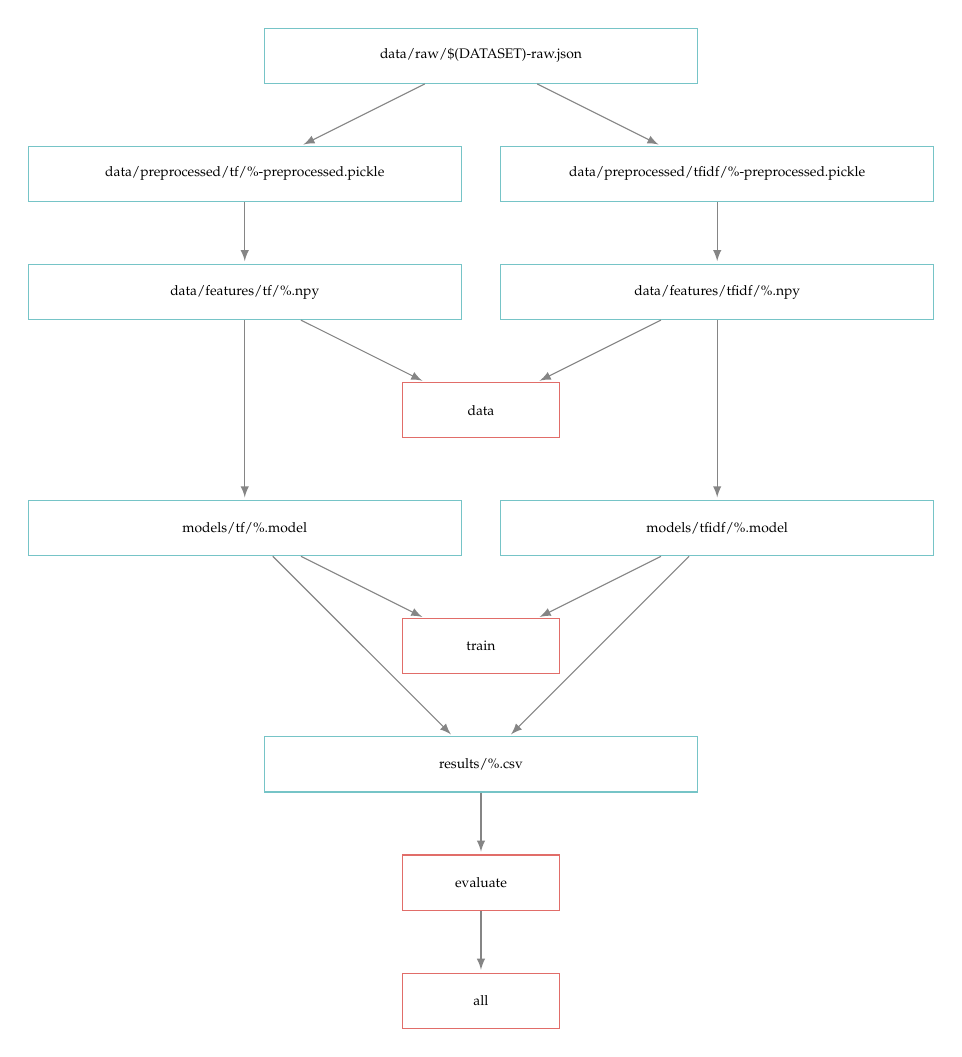
\begin{tikzpicture} [
    edge/.style={-latex,shorten >=1pt, thin, color=customGrey},
    line/.style={-,shorten >=1pt, thin, color=customGrey},
    fileTarget/.style={rectangle, draw=customBlue, align=left, minimum width=55mm, minimum height=7mm},
    phonyTarget/.style={rectangle, draw=customRed, align=left, minimum width=20mm, minimum height=7mm}
]

\node[fileTarget, align=center] (root) at (0, 0) {\tiny data/raw/\$(DATASET)-raw.json};

\node[fileTarget, align=center] (preprocessed_tf) at (-3, -1.5) {\tiny data/preprocessed/tf/\%-preprocessed.pickle};

\node[fileTarget, align=center] (preprocessed_tfidf) at (3, -1.5) {\tiny data/preprocessed/tfidf/\%-preprocessed.pickle};

\draw[edge] (root) -- (preprocessed_tf);
\draw[edge] (root) -- (preprocessed_tfidf);

\node[fileTarget, align=center] (features_tf) at (-3, -3) {\tiny data/features/tf/\%.npy};

\node[fileTarget, align=center] (features_tfidf) at (3, -3) {\tiny data/features/tfidf/\%.npy};

\draw[edge] (preprocessed_tf) -- (features_tf);
\draw[edge] (preprocessed_tfidf) -- (features_tfidf);

\node[phonyTarget, align=center] (data) at (0, -4.5) {\tiny data};

\draw[edge] (features_tf) -- (data);
\draw[edge] (features_tfidf) -- (data);

\node[fileTarget, align=center] (model_tf) at (-3, -6) {\tiny models/tf/\%.model};

\node[fileTarget, align=center] (model_tfidf) at (3, -6) {\tiny models/tfidf/\%.model};

\draw[edge] (features_tf) -- (model_tf);
\draw[edge] (features_tfidf) -- (model_tfidf);

\node[phonyTarget, align=center] (train) at (0, -7.5) {\tiny train};

\draw[edge] (model_tf) -- (train);
\draw[edge] (model_tfidf) -- (train);

\node[fileTarget, align=center] (results) at (0, -9) {\tiny results/\%.csv};

\draw[edge] (model_tf) -- (results);
\draw[edge] (model_tfidf) -- (results);

\node[phonyTarget, align=center] (evaluate) at (0, -10.5) {\tiny evaluate};

\draw[edge] (results) -- (evaluate);

\node[phonyTarget, align=center] (all) at (0, -12) {\tiny all};

\draw[edge] (evaluate) -- (all);

\end{tikzpicture}
   \caption{A dependency graph for a Makefile to perform experiments in our thesis. Blue rectangles represent \textit{file targets} and red rectangles represent \textit{phony targets}. Phony targets are targets that do not create or update a file, but instead represent a name for a sequence of commands to execute. Phony targets enable the modular execution of our experiments.}
	\label{fig:makefile}
	}
\end{figure}

Models and their configurations that are trained in the pipeline can be specified within the Makefile.

\subsubsection*{Scripts Implementation}
 A consistent file naming convention and file organization in directories and subdirectories is critical for automated experiments. For an example of the directory structure of our experiments designed for use with Makefile, see the Appendix \ref{appendix:dir_structure}.
 
 Each machine learning method has three Python scripts in the \texttt{src/models} directory: \textit{train}, \textit{evaluate}, and the \textit{model} itself. 
 
 Each \textit{model} script acts as a wrapper with a common interface that contains an algorithm-providing library (in our case, we use the LogLizer library, as described in Section \ref{subscetion:loglizer}) and allows calling the following methods:
 
\begin{itemize}
    \item \texttt{\_\_init\_\_}
    \item \texttt{fit}
    \item \texttt{predict}
    \item \texttt{evaluate}
    \item \texttt{save}
    \item \texttt{load}
\end{itemize}

The advantage of having a wrapper on top of the actual model is that it can easily be replaced by another library that provides the model implementation, or we can provide our own implementation.

As you can see from the list above, each model also contains \texttt{save} and \texttt{load} methods. They are included in the model as a means of serializing and deserializing the trained model. The reason for this is that training a model is usually a very time-consuming task. The ability to load an already trained model saves us the trouble of training the model every time it is needed. A serialized model can be conveniently restored later and used for evaluation or prediction. We use the library \texttt{pickle}\footnote{https://docs.python.org/3/library/pickle.html}, which converts any Python object into a byte stream. The process of serializing the data is then called "pickling" and the deserialization is called "unpickling".

\textit{Train} scripts allow optional and model-specific parameters to tune the models. These parameters can be modified in the Makefile. Then, the preprocessed data is simply loaded, the model is instantiated, and the model training process is executed. Finally, the trained model is stored in a pickle. 
 
\textit{Evaluate} scripts include loading the trained model and executing the \texttt{\justify evaluate} method to obtain metrics and predictions.

As shown in the directory structure in the Appendix \ref{appendix:dir_structure}, preprocessed features, trained models, and resulting metrics and predictions are stored in either the \texttt{tf} or \texttt{tfidf} folder, depending on which feature extraction method the particular file belongs to. \texttt{tf}, as an abbreviation for term frequency, is an equivalent to what we call \texttt{event count} in our work, as we explained in detail in Section \ref{subsection:features}. For brevity, we use \texttt{tf} in our file structure.

\subsection{Mapping from Prediction Back to Log Entry}
\label{methodology:mapping-predictions-back}
Once the output is computed, we get a prediction for each window of the input dataset. This is true regardless of the specific machine learning model used for the computation. 
This type of output, which consists of ones and zeros, is not very helpful if we want to understand why we got these results and whether they are correct. Ideally, we would want more detailed information about each window.
Typically, the windows that are identified as anomalous would be of interest, as they are expected to be less frequent and more important. However, there are use cases where we want to examine all windows, especially in the debugging phase. 

From a feature vector of a given window, only the ID and the frequency of the event type are given, the template and the order are lost.
After discussing with domain experts what would be valuable information about a time window, we concluded that it should be included with every window:
\begin{itemize}
    \item \textit{How frequent is each of the event types and what is the template for each event.}\\
    We create a histogram, ordered in descending order from the most frequent events to the least frequent. This gives a good overview of what the state of the system is in a given time window. 
    \item \textit{Raw trace of logs within the window.}\\
    The histogram is a good place to start, but in some cases the detail and preserved order matters. In some cases, we also need to know the variable parts of the log messages that are missing from the log templates to get a clear picture of what was going on in the system. Therefore, we also order the traces of the raw logs according to the time in which they occurred.
    \item \textit{What time range a window corresponds to.}\\
    It is easy to map from a window index to a human readable time. This way, an expert can tell if something special happened in the system. For example, regular tests may occur daily at certain times, which may explain some behavior.
\end{itemize}
 
% Flowchart: https://bost.ocks.org/mike/make/


\chapter{Dataset}
\label{chapter:dataset}

In this chapter we will provide information about the datasets we used in our research. We will describe how we obtained a labeled dataset for training and also mention the weaknesses associated with this dataset. We will take a look at the important properties of the logs. 
We will also discuss some known anomaly scenarios that can occur in the system logs, and we will go through the dataset in which they are captured. 
We use the anomalies to validate our models. A validation dataset that contains anomaly-free data will also be described. 

All datasets contain log traces collected from multiple microservices comprising the Motorola SmartConnect Cloud Infrastructure Engineering development environments.
To obtain the logs, we developed a pipeline (the details of the pipeline are described in Chapter~\ref{data_collection}) that connects to the system, collects logs, and preprocesses them into such a form that the data can be passed to selected machine learning algorithms or plotted.
More about the preprocessing step can be found in Chapter \ref{methodology}.

\section{Datasets}
\label{dataset}
The data we feed machine learning models with makes a big difference. Therefore, we need to look at what data we can collect at a high level from the system and what properties an individual log entry has.

The anomaly detection task can be reformulated as a classification problem with two classes: \textit{negative (anomaly)} class and \textit{positive (anomaly-free)} class. 

\textit{Negative} or \textit{normal} class is a category of a dataset that is free of anomalies and represents the expected (or normal) behaviour of a system that produces these logs. Negative data samples are labeled as $0$. The class \textit{Positive}, \textit{anomalous}, or \textit{abnormal} is the target class we are interested in. It is assigned to log sequences that contain anomalies as $1$. The goal is to train the classifier to distinguish between positive and negative samples.

Motorola Solution's policy for storing historical data is that we have logs available at any point in time from $30$ days ago to this point in time. The stored interval may at times become even smaller if the amount of persisted logs exceeds a limit.

In Motorola, the development environment is further divided into two subsections that we have access to. 
Let's call them \textit{experimental} and \textit{stable}. 

The \textit{stable} environment is synchronized with all the master branches of the source code. It is used to perform extensive testing of the system every night. 

On the other hand, the \textit{experimental} environment is used by the developers to deploy and explore side (or feature) branches during the day.

For confidentiality reasons, we do not have logs of the \textit{production} environment available. This is one of the major drawbacks, as it can be assumed that they contain different traffic. It can also be assumed that the distribution of anomalies in \textit{production} environment is different from both \textit{experimental} (more anomalies, some related to ad hoc deployment) and \textit{stable} (fewer anomalies, less traffic). In general, the development environment produces huge amounts of data, thousands of log messages per minute.

Next, we provide a detailed description of the characteristics of each dataset and how they were obtained. See Table \ref{table:datasets} for a summary of all datasets used in this work.

\subsection{Dataset Daily} 
This dataset reflects the \textit{experimental} region of the development environment. In such an environment, it is natural (or even desirable) for anomalies to occur.

We refer to the dataset of system logs produced by the region as the \textit{Daily} dataset, and may also refer to it as \textit{mixed}, since it will contain both positive and negative data samples. 
The system is active during a working day when developers are testing new features. The amount of logs varies greatly depending on the team's tasks. 
However, we are talking about tens of thousands of log messages per hour, even when the system is idle.

Unfortunately, such a dataset is not labeled, as experts would have to go through millions of lines of unstructured log messages to obtain the labels.

\subsection{Dataset Nightly}
At night, the system we are experimenting with goes through tests in the \textit{stable} region. This phase of health check of the system involves mimicking the normal behaviour of the telecommunications system. All the necessary infrastructure setup takes place and simulations of calls between groups of push-to-talk radios are performed. 
These tests are run again each night as part of the nightly test suite. 
Typically, the test pipeline lasts about 7 hours and produces about 2 million log messages.

If the nightly tests all pass, the data collected should either be completely free of anomalies, or contain only a very small percentage of them. 
Therefore, we assume that the data collected during the nightly testing phase, if passed successfully, will contain a large majority of negative data samples and represent normal anomaly-free behaviour of the system. This statement relies heavily on the assumption that the functionality of the system is well covered by the tests (the relationship of our approach to anomaly detection and test code coverage is discussed in detail in Section~\ref{code_coverage}). 

Therefore, for our use case, we can also interchangeably refer to the dataset \textit{Nightly} as \textit{negative} or \textit{normal} dataset.

Therefore, the logs collected at night by such a system should be suitable candidates for one-class classification algorithms as well as generate a labeled dataset for testing purposes, which we will explain later in this chapter.

However, the data generated by the system during nightly testing is slightly different from the live production environment. The main difference is that the scenarios generated by the test suite are serialized, meaning that there is at most one call at any given time. 

On the other hand, in the live production environment, there is no limit to the number of radio broadcasts at a time. Therefore, the logs of the production environment can contain much higher counts of some events.

Although this could be argued as a weakness of our nightly dataset, as described windowing operation of our preprocessing phase in Chapter~\ref{methodology}, we will always consider a sequence of logs and the number of event types in that log sequence in a fixed time window. Therefore, we believe that the final feature representation passed to the ML algorithm should be very similar, even though the data will look different with respect to individual log entries.

Since it is incredibly difficult to obtain labels in log data, we decided to use the Nightly data, despite its potential drawbacks and slightly artificial nature.

The Nightly data contains logs from the night of January 24, 2021.

\subsection{Dataset Nightly Test}
This dataset was collected in the same way as the Nightly and should meet all the properties, but it was recorded on a different day. Therefore, the timing is different and the tests are examining a different version of the SmartConnect system source code.

We use Nightly Test mainly to show that a similar distribution of arbitrary records collected during any nightly testing can be assumed.

Nightly Test contains logs from the night of January 22, 2021.

\subsection{Dataset Anomalies}

This dataset contains versions of the two anomaly scenarios described later in Section~\ref{anomaly_types}. 
The anomalies were achieved by killing Kubernetes Pods, which is responsible for the correct operation of a particular service type. 
At the same time, users were trying to establish, or were in a call.

This dataset captures a total of 23 instances of anomaly scenarios and was created by merging logs from two days - January 25 and 28, 2021.

\subsection{Dataset Glostrup Calling}

In contrast, the Glostrup Calling dataset consists of anomaly-free calls between Motorola Solutions two-way radios. 
The \textit{experimental} environment was set so that nothing else interferes with the calls. Therefore, the resulting logs can be considered as \textit{normal} data.

The trace records several calls that were carried out during 8 minutes on February 3, 2021.

\section{Dataset Test with Labels} 
\label{section:testset}
Unsupervised learning does not require data to be labeled to detect anomalies, as it assumes that the majority of data points are normal.  This is very beneficial in our situation where it is extremely difficult to obtain labeled data. However, the lack of labels poses a difficulty when it comes to the model evaluation phase.

Unlike supervised learning, where one can directly compare predictions with actual labels to assess the quality of the machine learning model, there is no way to do this in unsupervised learning.

In our work, the majority of the data is unlabeled data. To validate the proposed approaches, we had to develop the test dataset ourselves.

To get a better idea of what kind of data constitutes a manually created test dataset, we provide a pie chart of the test set composition in Figure \ref{fig:testset-composition}. It is important to note that the number $131$ represents the amount of extracted log sequence, so the number of underlying log message samples is much higher.

Determining the negative class representation is trivial. As we mentioned earlier in this chapter, we consider the Nightly data from the testing phase as normal data samples. To create the normal part of the dataset, we collect another set of data from the testing phase that was previously unseen in the training phase. 

On the other hand, positive samples must be manually labeled. To avoid label assignment errors, we introduce some known anomaly scenarios that are expected to occur in our real dataset. These scenarios can be reproduced, we can collect the data and label them as anomalies. 

This is not an ideal test dataset, but not all anomalies are known and can be sourced. It provides a reasonable tool to measure how well our models are performing. We will also test the models with only normal data to detect false positives. 

\begin{figure}[h]
    \centering
    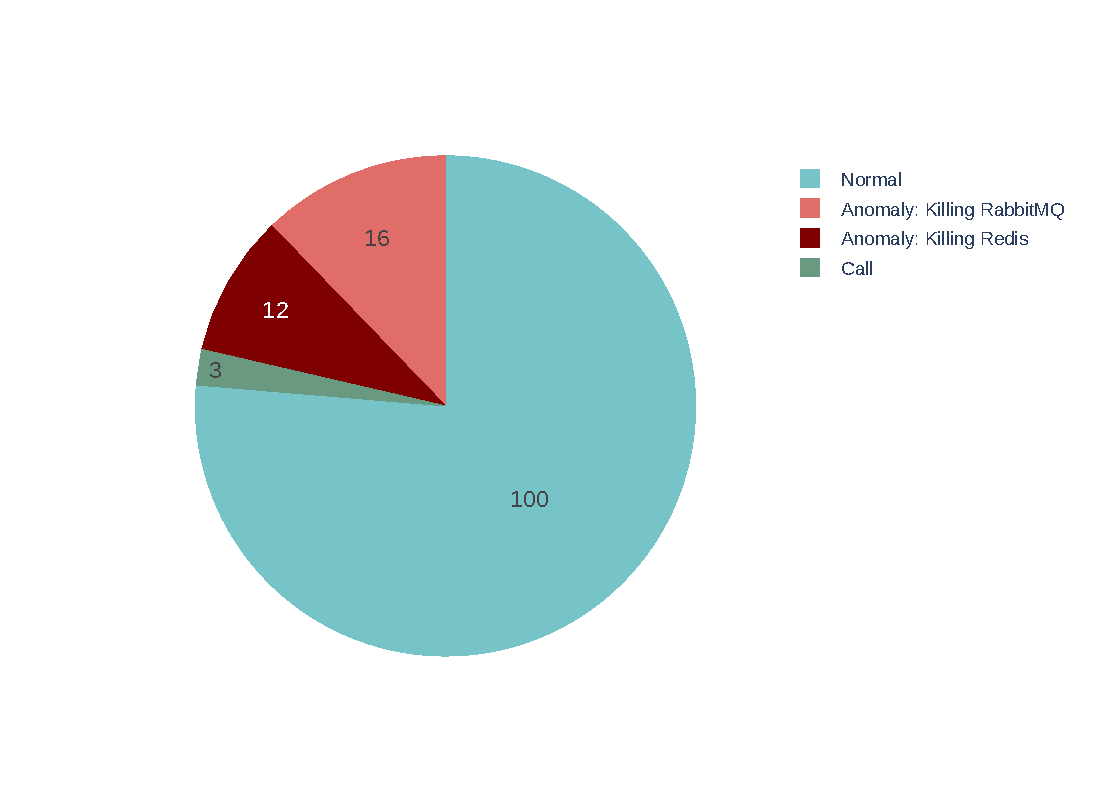
\includegraphics[width=0.8\textwidth]{img/testset-composition.pdf}
    \caption{Testing dataset composition. A manually collected and labeled dataset consists of 131 log sequences, where each log sequence was collected within a two-minute time window. The value in each section of the pie chart indicates the number of log sequences of each type of log message it contains. The "Normal" and "Call" sections of the pie chart both represent normal, anomaly-free behaviour, while " Killing RabbitMQ" and "Killing Redis" are anomalies.}
    \label{fig:testset-composition}
\end{figure}

\begin{table}[!h]
\centering
\resizebox{\textwidth}{!}{\begin{tabular}{@{}lcr@{}}
\toprule
\textbf{Dataset Name} & \textbf{Log Entries}       & \textbf{Size}  &\textbf{Time Span}  \\ \toprule
\textcolor{customDarkBlue}{\textbf{Daily}}           & $539\,372$    & $2.84$ GB     & \footnotesize{ 26/1/2021 6:00  -  26/1/2021 21:00 }     \\ \midrule
\textcolor{customDarkBlue}{\textbf{Nightly}}         & $1\,362\,004$ & $4.24$ GB     &  \footnotesize{24/1/2021 21:00  -  25/1/2021 3:50}      \\ \midrule
\textcolor{customDarkBlue}{\textbf{Nightly Test}}    & $1\,373\,919$ & $4.47$ GB     &  \footnotesize{22/1/2021 21:00  -  23/1/2021 3:43}      \\ \midrule
\textcolor{customDarkBlue}{\textbf{Anomalies}}       & $805\,614$    & $3.6$ GB      & \footnotesize{ 25/1/2021 15:40  -  25/1/2021 17:00,  28/1/2021 15:25  -  28/1/2021 16:00}    \\ \midrule
\textcolor{customDarkBlue}{\textbf{Glostrup Calling}}    & $1904$    & $15.82$ MB    &  \footnotesize{3/2/2021 9:40  -  3/2/2021 9:47} \\
\bottomrule
\end{tabular}}
\caption{Summary of all the log datasets we worked with in our research on anomaly detection.}
\label{table:datasets}
\end{table}

\section{Log Properties}
The services record 33 properties per single log entry. Of the 33 log properties, we chose to consider only \texttt{msg} and \texttt{timestamp}, as the others (such as the name of the Kubernetes pod, the process ID of the service generating the log, etc.) are too specific. For the full list of the individual log properties see Appendix~\ref{appendix:log-properties}).
Including fewer predictor variables should generally avoid overfitting, make the final model more transparent, and make debugging easier.
Therefore, to obtain as general a solution as possible, we restrict ourselves to these two predictors.

\subsection{Format of Log Properties}
Messages are strings and we assume that they follow the logic we described in Section~\ref{log_template_mining} on log template mining. In other words, we assume that they are generated by code in such a way that they can be thought of as a product of constant and variable parts. Consequently, log messages can be further categorized using event types.

Timestamps have the format of \texttt{YYYY-MM- DD'T'HH:mm: SS.sss'Z'}. The format string indicates that the year (YYYY) is a four-digit number padded with zeros, the month (\texttt{MM}), the day (\texttt{ DD }), the hour (\texttt{HH}), the minutes (\texttt{mm}) and the seconds (\texttt{ SS }) are two-digit zero padded numbers and the milliseconds (\texttt{ssss}) are a three-digit number filled with zeros. The time part is separated from the date by a single \texttt{T} character and the entire timestamp ends with a letter \texttt{Z}.

\section{Types of Anomalies}
\label{anomaly_types}
In this section, we present a set of known anomalies that we will trace in order to test our solution.
We will benchmark our approaches and models to these known anomalies, which can be easily simulated and reproduced. 
However, the goal is to also detect anomalies that we are not aware of.
In other words, we also want to identify anomalous scenarios that appear for the first time in the production environment and do not appear in our training and testing dataset.

\subsection{Cache Outage}
In this anomaly, a cache storage that orchestrates the call logic is taken down and the radios that are in a call at that moment bonk because they cannot communicate with each other.
In response, the storage service automatically restores itself, usually in no more than 2 seconds. After that, broadcast should continue.

As mentioned in Section~\ref{architecture:caching} about caching in Motorola SmartConnect, Redis is used for caching, so we can also call this anomaly \textit{ Killing Redis } or similar.

\subsection{Message Broker Out of Service}
Similarly, an important entity in the SmartConnect microservices system is the message broker that enables inter-service communication. In this scenario, all brokers are terminated, therefore the microservices network is disrupted and messages cannot be forwarded until the brokers are restored.

Section~\ref{architecture:messaging} discusses again how messages are forwarded in SmartConnect's microservices architecture. RabbitMQ is the specific message broker that is used, so we can refer to this anomaly in the text as \textit{Killing RabbitMQ}.

% https://pure.tue.nl/ws/portalfiles/portal/142685995/sci_2019_Lomagin_Egor.pdf
\chapter{Experiments}
\chapter{Results}

\chapter{Conclusions and Future Work}
\label{conclusion}
In our work, we have attempted to apply anomaly detection to a real-world dataset obtained in collaboration with Motorola Solution's Smart Connect. We have formulated a methodology for analyzing unstructured system log data. 

Our methodology workflow is initiated by \textit{data collection}. The implemented solution to collect log data produced by SmartConnect's microservices queries Elasticsearch within the cluster. We collected data instances representing the normal behavior of the system, as well as some known anomalies that we simulated on site.

Since logs typically contain variable parts that result in different log messages for the same log event type, a \textit{log parsing} technique is used to extract unique log event types. For this purpose, an online parser of the Drain3 library is used. 

We have proposed two different approaches for \textit{feature extraction}, namely the event count vector and the weighted TF-IDF vector. Both representations are generated from two minute windows. In each time window, the occurrence of unique event types is counted and in the case of TF-IDF, the counts are weighted. It has been shown that both representations perform similarly well.

Finally, we examined and compared four different \textit{anomaly detection} models, along with an analysis of their architecture and hyperparameter selection. Model evaluation was a problematic part of our research, due to the lack of known anomaly scenarios to test and thus a lack of data labels as well. We performed an evaluation of the selected algorithms on a task of unsupervised one-class anomaly detection on log data on a small, manually generated test dataset with two known anomalies. In a second step of the evaluation, we asked experts to assess the predicted labels for unknown anomalies. We concluded that simple algorithms, such as Log Clustering and PCA, performed very well on the test dataset.

During our research, we made the following main contributions:

\begin{itemize}
    \item Demonstrated the applicability of our methodology to real-world case analysis
    \item Implemented core anomaly detection components, that can be used for future anomaly detection pipeline in production dataset in Smart Connect
\end{itemize}

\section{Conclusion}

\addcontentsline{toc}{chapter}{Conclusion}
In our research, we reviewed and tried four unsupervised anomaly detection methods to prove that outlier detection using machine learning techniques can be applied to log data in the domain of MSI's SmartConnect product.

Based on the conducted results of the experiments on the feature extraction methods proposed in our work on Motorola Solutions data, we can answer the research questions outlined in Chapter \ref{introduction}. In the remainder of the chapter, we will provide a short answer to each of the research questions.

We focused on detecting anomalies that were known to us before conducting the experiments. We attempted to prove that our algorithms could detect them and while not triggering error when normal events occured. However, the desired application of our solution would be to be able to detect anomalies by monitoring the system in real time. In the section below, we will elaborate the rough workflow of how the alarms would be raised in the future anomaly detection pipeline. For this use-case, it would be worthwhile to experiment with smaller windows and possibly overlapping windows, as opposed to the strict fixed-size embedding we are doing at the moment. The reason for looking at smaller windows is that a finer granularity of problems could be detected this way. If an anomaly occurs, the system breaks down, and users suffer, it is no longer as useful to detect an anomaly because the system has been severely impacted. However, if the window is small enough to capture an event that leads to an anomaly, something can be done about the initial problem at some point to prevent the entire anomaly (consisting of $n, n > 1$ windows) from occurring.

\textbf{RQ1}: \textit{\RQFirst}\\

Before the actual process of active anomaly detection, we performed an initial exploration of the dataset. After we plotted the two types of observed anomalies, killing Redis and killing RabbitMQ, on top of the Nightly dataset of normal instances (Figure \ref{fig:tsne-anomalies}), the plot showed three distinct clusters. Each cluster contained similar data points (log sequences) grouped into clusters, and the cluster of normal instances was separated from the cluster of anomalous instances, based on the behaviour of the underlying data points. In addition, visual interpretation also allowed us to distinguish between two different types of anomalies.

Being able to see anomalies with the naked eye gives us the "why" of a particular decision made by the anomaly detection algorithm. Interpretability and explainability in machine learning is extremely important. It helps us to understand what the reasons are for the results, and it also helps us trust the final models.

Therefore, we argue that visual analysis is direct evidence that the dataset of logs produced by Motorola Solutions SmartConnect contains enough information for anomaly detection and the answer to the first research question is \textbf{yes}. \\

\textbf{RQ2}: \textit{\RQSecond}\\

As part of our research, we designed a preprocessing stage that transfers unstructured log messages into a structured format, or \textit{embedding}. We proposed two different types of feature embeddings: an event count vector and TF-IDF weighted vector.

To answer this question, we conducted machine learning experiments and discovered that our best performing models can successfully detect all types of known anomalies, with an F1 score of $100 \%$ on the test dataset.

Both types of feature embeddings performed similarly well, however we choose to prefer the event count embedding due to its simplicity in terms of generation and interpretation. It seems that a simple representation in the context of the frequency of different event counts is detailed enough to detect outliers within the normal data. 

These results confirm that this type of feature extraction, which is commonly used in anomaly detection, successfully reflects the characteristics of SmartConnect log messages for further outlier analysis.\\

\textbf{RQ3}: \textit{\RQThird}\\

To answer the third research question, we conducted a thorough investigation of anomaly detection methods, approaches, and similar research papers, in which they have been successfully used. The architecture of the anomaly detection process consists of many more steps than just the selection and execution of an ML algorithm. 

We proposed a workflow of our research that consists of four important steps: Data collection, Log parsing, Feature Engineering and Anomaly Detection.

As a result of our research, we have compiled a short list of four representative state-of-the-art algorithms for unsupervised anomaly detection, including Isolation Forest, PCA, Invariants Mining and Log Clustering. Based on the research results, we investigated several log parsing algorithms, that are also a critical component of successful anomaly detection. We chose to use an online log parser called Drain3.\\

\textbf{RQ4}: \textit{\RQFourth}\\

With the accumulated knowledge to convert data into a structured format and verify our assumption using data visualization techniques, we were ready to perform the final part of the research - conducting experiments. To find the ideal parameters for anomaly detection algorithms, we performed a simple grid search over the hyperparameter space. We did not care to explore the hyperparameters in detail, as achieving optimal parameters and results was not the main goal of this work. 

Anomaly detection algorithms are judged on their ability to correctly identify anomalies. To measure this ability, we used four types of evaluation metrics: Precision, Recall, F1 Score and Accuracy. On the test set, the log clustering and PCA algorithms are able to detect $100 \%$ of killing Redis and killing RabbitMQ anomalies and $100 \%$ of normal data instances. A special type of normal samples are calls between two radios, which appeared as outliers on some plots, are also correctly detected as anomaly-free. 

The killing Redis and RabbitMQ anomalies are realtively easy to detect due to the logs generated and the high volumes generated on these occasions. However, reproducing anomalies in the SmartConnect system is not a trivial task. The data from these two cases of anomalies were obtained on site physically making the calls while stopping the connection to the Redis and RabbitMQ services, when the experimental environment was not interrupted by other experiments performed by developers. 
We also argue that being able to recognize these two anomalies and distinguish them from each other is helpful information that it is possible to detect an occurrence of anomalies in this dataset. 

To support this claim, we leveraged the knowledge of domain experts - developers in the SmartConnect team to evaluate the discovered results on dataset with unknown number and type of anomalies. In this way, we obtained an unbiased view of the performance of the trained models. Due to the high number of logs in time windows that the experts were asked to examine, they could not confidently confirm the predicted labels of all time windows. However, they managed to find another anomaly cluster, that was correctly identified as an anomaly by PCA. The anomaly represented by this cluster was unknown before the experiment.

\section{Weaknesses and Limitations}
Although we have been able to achieve some great results and discoveries during our methodological process, there are a number of possible improvements that could be made.
In this section we will address some of the weaknesses and limitations that we encountered during our research.

\subsection{Evaluation}
First and foremost, the most difficult part in anomaly detection is actually verifying the results because our labeled dataset and the set of known anomalies have a very limited size. 
For this reason, we were unable to draw conclusions about performance on a real-world dataset. However, due to the complexity of the log data, this was not possible, as labeling the data is extremely time consuming. We asked experts to manually validate of the predictions on an experimental dataset. They approved of the reported anomalies and did not report any false negatives. 

However, relying on a human being as the one to validate the actual results and performance makes the whole process more error-prone and even more time consuming.

\subsection{Dataset}
The major limitation of our research is that we were not able to verify our results using datasets from the live production environment. Instead, we used log data generated in a test and experimental environment.
This is due to the fact that log data generated in the production environment is highly confidential as it may contain information that can be easily exploited if not handled properly. 

To overcome this, a strategy for anonymous handling and storage of data in our program needs to be developed, which is beyond the scope of this paper.

\subsection{Optimal Window Size}
Another issue that has not been fully addressed in this paper is further experimentation with the relationship between performance and window size. 
In our study, we only worked with embedding in time windows with a fixed time of two minutes and the windows were non overlapping.
It can be argued, that since the downtime caused by anomalies, which we primarily studied, is less than two minutes, our solutions should perform reasonably well.
However, it remains to be explored how this embedding choice would cope with particularly longer lasting anomalies.

\subsection{Variant Length of Feature Vector}
In the feature engineering step, we embed features into an event count matrix, where we mark how many times an event occurred in a given time window. However, when embedding previously unseen records, it will eventually happen that a previously unseen event occurs and thus the length of the feature vector increases. In the current solution, when this happens, we have to go back and re-train our models to match the new vector size. 

To make our solution more robust, an additional column should be introduced in the feature vector. The frequency of this event type would be incremented whenever an event occurs that was not represented in the training data. 
After that, in the model re-training step (which is suggested as a possible extension in Section~\ref{future:pipeline}) the new event types integrated and the event count would be properly increased.

\section{Future Work}
In the time frame of six months, we we able to prove that applying machine learning based monitoring tools to detect anomalies in Motorola SmartConnect is well possible.
However, many interesting questions arose along the way that we could not address within the scope of this project.
Also, our solution should not be considered a finished product that can be packaged and shipped. Definitely, more software engineering work needs to be done before we can claim that. For now, our solution is mainly for experimental purposes.
Here we describe the questions whose answers need to to be explored in future research.

\subsection{Anomaly Detection Pipeline}
\label{future:pipeline}
As described earlier in Section~\ref{dataset}, so far our anomaly detection tool only observes the experimental environment intended for developers to try out new features. 

This is only a proof-of-concept for our solution. To take full advantage of an automated anomaly detection product, it needs be deployed in the production environment. However, in a large company like Motorola Solution, this takes more than just a few months, which we had available for this work.

Let us illustrate what processes are required to improve our solution so that it can be useful in production.

First, we need to develop a proper pipeline for continuous training of the model(s). We have the foundation in place, but, what remains to be done is to automate the process that checks if the nightly tests passed correctly, and if so, the log samples from that night are downloaded, labeled, and added to the training dataset. The model needs to be re-trained and updated in production. At this stage, the question of how much training is too much also needs to be addressed.

At the same time, our research has not addressed what the specific ways would be to trigger an alarm  each time an anomaly is found. Then, a mechanism must be triggered to deal with the detected problem, whether it is a program that attempts to heal the problem or the notification of a person responsible for observing the state of the system.

\subsection{Code Coverage}
\label{code_coverage}
After becoming familiar with the Motorola SmartConnect system, we decided to use one-class learning (classification) methods to detect anomalies.
Domain knowledge proved critical as it allowed us to take advantage of the fact that we could collect data from nightly tests. 
We then selected machine learning algorithms that we fed only negative data.

We based our solution on some assumptions about the logs we collect from passing tests:
\begin{enumerate}

    \item If a test passes, it contains no anomalies.
    %\item The code under the test is actually related to the one that is being monitored.
    \item The tests cover the code “sufficiently” and largely examine the data paths that can be executed within the system. 

\end{enumerate}

The first assumption basically says that even if the tests mimic scenarios where a failure is simulated and the system can recover from that failure, we do not want to consider that an anomaly. 
In this case, no alarm is raised because the system does not require human intervention and is prepared to handle the problem.

The last point brings us to an interesting feature of our solution, which opens a whole new perspective that can be explored in future research.

By the nature of the embedding chosen and the machine learning methods studied, the models run into trouble in case when there is an anomaly free scenario that was not sufficiently present in the training dataset (or better, could not be inferred from the dataset). If this non-anomalous scenario then shows up in the system monitored by our anomaly detection tool, false positives will result.\\
In our case, however, we can rephrase the statement into the claim that if the model frequently reports anomalies that are not in fact anomalies (false positives), this can be turned into valuable information about the tests themselves. 
More specifically, it means that the tests are not examining some properties of the system and are prone to introducing errors into the product. 
This observation, along with our anomaly detection solution, can be used as the basis for a tool that could be plugged into a system monitoring process.


%%% Bibliography
  
%%% Bibliography (literature used as a source)
%%%
%%% We employ bibTeX to construct the bibliography. It processes
%%% citations in the text (e.g., the \cite{...} macro) and looks up
%%% relevant entries in the bibliography.bib file.
%%%
%%% The \bibliographystyle command selects, which style will be used
%%% for references from the text. The argument in curly brackets is
%%% the name of the corresponding style file (*.bst). Both styles
%%% mentioned in this template are included in LaTeX distributions.

%\bibliographystyle{plainnat}    %% Author (year)
\bibliographystyle{unsrt}     %% [number]

\renewcommand{\bibname}{Bibliography}

%%% Generate the bibliography. Beware that if you cited no works,
%%% the empty list will be omitted completely.

\bibliography{bibliography}

%%% If case you prefer to write the bibliography manually (without bibTeX),
%%% you can use the following. Please follow the ISO 690 standard and
%%% citation conventions of your field of research.

% \begin{thebibliography}{99}
%
% \bibitem{lamport94}
%   {\sc Lamport,} Leslie.
%   \emph{\LaTeX: A Document Preparation System}.
%   2nd edition.
%   Massachusetts: Addison Wesley, 1994.
%   ISBN 0-201-52983-1.
%
% \end{thebibliography}


%%% Figures used in the thesis (consider if this is needed)
\listoffigures

\begin{appendices}
\chapter{Dataset}

\section{Log Properties List}
\label{appendix:log-properties}
\begin{enumerate}
\item @timestamp

\item \textunderscore id
	
\item \textunderscore index
	
\item \textunderscore score

\item \textunderscore type
	
\item agent.ephemeral\textunderscore id
	
\item agent.hostname
	
\item agent.id
	
\item agent.type
	
\item agent.version
	
\item cloud.instance.id
	
\item cloud.instance.name
	
\item cloud.machine.type
	
\item cloud.provider
	
\item cloud.region
	
\item ecs.version
	
\item host.name
	
\item input.type
	
\item kubernetes.container.image
	
\item kubernetes.container.name
	
\item kubernetes.labels.app
	
\item kubernetes.labels.ignore-drain
	
\item kubernetes.labels.pdb
	
\item kubernetes.labels.pod-template-hash
	
\item kubernetes.namespace
	
\item kubernetes.node.name
	
\item kubernetes.pod.name
	
\item kubernetes.pod.uid
	
\item kubernetes.replicaset.name
	
\item log.file.path

\item log.offset
	
\item message
	
\item stream

\end{enumerate}
\chapter{Experiments}

\section{Experimental Setup}

\subsection{Hyperparameter Tuning}
\label{appendix:hyperparameterTuning}
\subsubsection{Log Clustering}
\begin{table}[h]
\centering
\resizebox{\textwidth}{!}{\begin{tabular}{@{}cccccc@{}}
\toprule
Max distance & Anomaly threshold & \textbf{Precision} & \textbf{Recall} & \textbf{F1} & \textbf{Accuracy} \\ \midrule
0.3          & 0.3               & 100.00\%                  & 100.00\%               & 100.00\%           & 100.00\%                 \\
0.3          & 0.5               & 100.00\%                  & 100.00\%               & 100.00\%           & 100.00\%                 \\
0.5          & 0.3               & 100.00\%                  & 100.00\%               & 100.00\%           & 100.00\%                 \\
0.5          & 0.5               & 100.00\%                  & 100.00\%               & 100.00\%           & 100.00\%                 \\ \bottomrule
\end{tabular}}
    \caption{Precision, Recall, F1-score and Accuracy of the test dataset on Log Clustering model with different hyperparameter values.}
    \label{tab:pca_tuning}
\end{table}

\subsubsection{Invariants Mining}

\begin{table}[h]
\centering
\begin{tabular}{@{}cccccc@{}}
\toprule
Percentage & Epsilon & \textbf{Precision} & \textbf{Recall} & \textbf{F1} & \textbf{Accuracy} \\ \midrule
0.98       & 5       & 22.22\%               & 100.00\%               & 36.36\%      & 25.19\%            
\end{tabular}
    \caption{Precision, Recall, F1-score and Accuracy of the test dataset on Invariants Mining model and its hyperparameter values.}
    \label{tab:pca_tuning}
\end{table}

\subsubsection{PCA}

\begin{table}[h]
\centering
\resizebox{\textwidth}{!}{\begin{tabular}{@{}ccccccc@{}}
\toprule
Number of components & Threshold & Alpha  & \textbf{Precision} & \textbf{Recall} & \textbf{F1} & \textbf{Accuracy} \\ \midrule
0.85                 & auto      & 0.0001 & 100.00\%           & 75.00\%         & 85.71\%     & 94.66\%           \\
0.85                 & auto      & 0.001  & 100.00\%           & 85.71\%         & 92.30\%     & 96.95\%           \\
0.85                 & auto      & 0.005  & 100.00\%           & 92.86\%         & 96.30\%     & 98.47\%           \\
0.85                 & auto      & 0.01   & 100.00\%           & 92.86\%         & 96.30\%     & 98.47\%           \\
0.90                 & auto      & 0.0001 & 100.00\%           & 75.00\%         & 85.71\%     & 94.66\%           \\
0.90                 & auto      & 0.001  & 100.00\%           & 85.71\%         & 92.31\%     & 96.94\%           \\
0.90                 & auto      & 0.005  & 100.00\%           & 92.86\%         & 96.30\%     & 98.47\%           \\
0.90                 & auto      & 0.01   & 100.00\%           & 92.86\%         & 96.30\%     & 98.47\%           \\
0.95                 & auto      & 0.0001 & 100.00\%           & 92.86\%         & 96.30\%     & 98.47\%           \\
0.95                 & auto      & 0.001  & 100.00\%           & 96.43\%         & 98.18\%     & 99.23\%           \\
\textcolor{customDarkRed}{\textbf{0.95}}                 & \textcolor{customDarkRed}{\textbf{auto}}      &  \textcolor{customDarkRed}{\textbf{0.005}} & \textcolor{customDarkRed}{\textbf{100.00\%}}           & \textcolor{customDarkRed}{\textbf{100.00\%}}        & \textcolor{customDarkRed}{\textbf{100.00\%}}    & \textcolor{customDarkRed}{\textbf{100.00\%}   }      \\
\textcolor{customDarkRed}{\textbf{0.95}}                 & \textcolor{customDarkRed}{\textbf{auto}}      & \textcolor{customDarkRed}{\textbf{0.01}}   & \textcolor{customDarkRed}{\textbf{100.00\%}}          & \textcolor{customDarkRed}{\textbf{100.00\%}}        & \textcolor{customDarkRed}{\textbf{100.00\%}}    & \textcolor{customDarkRed}{\textbf{100.00\%}}          \\ \bottomrule
\end{tabular}}
    \caption{Precision, Recall, F1-score and Accuracy of the test dataset on PCA model with different hyperparameter values.}
    \label{tab:pca_tuning}
\end{table}

\subsubsection{Isolation Forest}
\begin{table}[h]
\centering
\resizebox{\textwidth}{!}{\begin{tabular}{cccccccc}
\hline
Number of estimators & Max samples & Contamination & Max features & \textbf{Precision} & \textbf{Recall} & \textbf{F1} & \textbf{Accuracy} \\ \hline
50                   & 150         & 0             & 3693         & 100.00\%           & 10.71\%         & 19.35\%     & 80.92\%           \\
50                   & 150         & 0.02          & 3693         & 66.67\%            & 7.14\%          & 12.90\%     & 79.34\%           \\
50                   & 150         & 0.03          & 3693         & 50.00\%            & 14.29\%         & 22.22\%     & 78.63\%           \\
50                   & 150         & 0.1           & 3693         & 71.42\%            & 3.57\%          & 4.76\%      & 69.47\%           \\
50                   & 180         & 0             & 3693         & 0.00\%             & 0.00\%          & 0.00\%      & 78.63\%           \\
50                   & 180         & 0.02          & 3693         & 0.00\%             & 0.00\%          & 0.00\%      & 76.33\%           \\
50                   & 180         & 0.03          & 3693         & 33.33\%            & 7.14\%          & 11.76\%     & 77.10\%           \\
\textcolor{customDarkRed}{\textbf{50}}                   & \textcolor{customDarkRed}{\textbf{180}}        & \textcolor{customDarkRed}{\textbf{0.1}}           & \textcolor{customDarkRed}{\textbf{3693}}        & \textcolor{customDarkRed}{\textbf{80.00\%}}            & \textcolor{customDarkRed}{\textbf{57.14\%}}         & \textcolor{customDarkRed}{\textbf{66.67\%}}    & \textcolor{customDarkRed}{\textbf{87.79\%}}          \\
50                   & 201         & 0             & 3693         & 78.63\%            & 0.00\%          & 0.00\%      & 0.00\%            \\
50                   & 201         & 0.02          & 3693         & 66.67\%            & 14.23\%         & 23.53\%     & 80.15\%           \\
50                   & 201         & 0.03          & 3693         & 0.00\%             & 0.00\%          & 0.00\%      & 75.57\%           \\
50                   & 201         & 0.1           & 3693         & 0.00\%             & 0.00\%          & 0.00\%      & 67.94\%           \\
100                  & 150         & 0             & 3693         & 0.00\%             & 0.00\%          & 0.00\%      & 78.63\%           \\
100                  & 150         & 0.02          & 3693         & 57.14\%            & 14.23\%         & 22.86\%     & 79.39\%           \\
100                  & 150         & 0.03          & 3693         & 40.00\%            & 7.14\%          & 12.12\%     & 77.86\%           \\
\textcolor{customDarkRed}{\textbf{100}}                  & \textcolor{customDarkRed}{\textbf{150}}         & \textcolor{customDarkRed}{\textbf{0.1}  }        & \textcolor{customDarkRed}{\textbf{3693}}         & \textcolor{customDarkRed}{\textbf{65.51\%}}            & \textcolor{customDarkRed}{\textbf{67.86\%}}         & \textcolor{customDarkRed}{\textbf{66.67\%}}    & \textcolor{customDarkRed}{\textbf{85.50\%}}           \\
100                  & 180         & 0             & 3693         & 0.00\%             & 0.00\%          & 0.00\%      & 78.63\%           \\
100                  & 180         & 0.02          & 3693         & 0.00\%             & 0.00\%          & 0.00\%      & 77.86\%           \\
100                  & 180         & 0.03          & 3693         & 0.00\%             & 0.00\%          & 0.00\%      & 76.34\%           \\
100                  & 180         & 0.1           & 3693         & 0.00\%             & 0.00\%          & 0.00\%      & 71.76\%           \\
100                  & 201         & 0             & 3693         & 100.00\%           & 3.57\%          & 6.90\%      & 79.39\%           \\
100                  & 201         & 0.02          & 3693         & 90.00\%            & 32.14\%         & 47.37\%     & 84.73\%           \\
100                  & 201         & 0.03          & 3693         & 50.00\%            & 7.14\%          & 12.50\%     & 78.63\%           \\
100                  & 201         & 0.1           & 3693         & 66.67\%            & 50.00\%         & 57.14\%     & 83.97\%           \\
150                  & 150         & 0             & 3693         & 0.00\%             & 0.00\%          & 0.00\%      & 78.63\%           \\
150                  & 150         & 0.02          & 3693         & 50.00\%            & 7.14\%          & 12.50\%     & 78.63\%           \\
150                  & 150         & 0.03          & 3693         & 33.33\%            & 7.14\%          & 11.76\%     & 77.10\%           \\
150                  & 150         & 0.1           & 3693         & 33.33\%            & 21.42\%         & 26.10\%     & 74.04\%           \\
150                  & 180         & 0             & 3693         & 0.00\%             & 0.00\%          & 0.00\%      & 78.63\%           \\
150                  & 180         & 0.02          & 3693         & 66.67\%            & 7.14\%          & 12.90\%     & 79.38\%           \\
150                  & 180         & 0.03          & 3693         & 50.00\%            & 14.29\%         & 22.22\%     & 78.63\%           \\
150                  & 180         & 0.1           & 3693         & 43.75\%            & 25\%            & 31.82\%     & 77.10\%           \\
150                  & 201         & 0             & 3693         & 0.00\%             & 0.00\%          & 0.00\%      & 78.63\%           \\
150                  & 201         & 0.02          & 3693         & 50.00\%            & 7.14\%          & 12.50\%     & 78.63\%           \\
150                  & 201         & 0.03          & 3693         & 0.00\%             & 0.00\%          & 0.00\%      & 76.34\%           \\
150                  & 201         & 0.1           & 3693         & 20.00\%            & 10.71\%         & 13.95\%     & 71.76\%           \\
201                  & 150         & 0             & 3693         & 0.00\%             & 0.00\%          & 0.00\%      & 78.63\%           \\
201                  & 150         & 0.02          & 3693         & 77.78\%            & 25.00\%         & 37.84\%     & 82.44\%           \\
201                  & 150         & 0.03          & 3693         & 71.43\%            & 17.43\%         & 28.57\%     & 80.92\%           \\
201                  & 150         & 0.1           & 3693         & 35.30\%            & 21.43\%         & 26.67\%     & 74.81\%           \\
201                  & 180         & 0             & 3693         & 0.00\%             & 0.00\%          & 0.00\%      & 78.63\%           \\
201                  & 180         & 0.02          & 3693         & 50.00\%            & 7.14\%          & 12.50\%     & 78.63\%           \\
201                  & 180         & 0.03          & 3693         & 40.00\%            & 7.14\%          & 12.12\%     & 77.86\%           \\
201                  & 180         & 0.1           & 3693         & 38.89\%            & 25.00\%         & 30.43\%     & 75.57\%           \\
201                  & 201         & 0             & 3693         & 0.00\%             & 0.00\%          & 0.00\%      & 78.63\%           \\
201                  & 201         & 0.02          & 3693         & 66.67\%            & 14.29\%         & 23.53\%     & 80.15\%           \\
201                  & 201         & 0.03          & 3693         & 42.86\%            & 10.71\%         & 17.14\%     & 77.86\%           \\
201                  & 201         & 0.1           & 3693         & 57.69\%            & 53.57\%         & 55.56\%     & 81.68\%          
\end{tabular}}
    \caption{Precision, Recall, F1-score and Accuracy of the test dataset on Isolation Forest model with different hyperparameter values.}
    \label{tab:pca_tuning}
\end{table}

\newpage
\subsection{Directory structure used with Makefile}
\label{appendix:dir_structure}
 
 \dirtree{%
.1 /. 
.2 data. 
.3 features. 
.4 tf. 
.4 tfidf. 
.3 labels. 
.3 preprocessed. 
.3 raw. 
.2 models. 
.3 tf. 
.3 tfidf. 
.2 results. 
.3 metrics. 
.4 tf. 
.4 tfidf. 
.3 predictions. 
.4 tf. 
.4 tfidf. 
.2 src. 
.3 data. 
.4 categorization.py. 
.4 feature\textunderscore extraction.py. 
.4 template\textunderscore mine.py. 
.3 models. 
.4 invariant\textunderscore mining.py. 
.4 isolation\textunderscore forest.py. 
.4 log\textunderscore clustering.py. 
.4 train.py. 
.4 evaluate.py. 
.4 pca.py. 
.2 Makefile. 
}

\subsection{Makefile for running experiments}
\label{appendix:makefile}

\lstset{language=[gnu] make}
\begin{lstlisting}
.PHONY: all clean data train evaluate

#################################################
# GLOBALS                                       #
#################################################

RAW_DATA_DIR=data/raw/
PREPROCESSED_DATA_DIR=data/preprocessed/
FEATURES_DATA_DIR=data/features/
LABELS_DATA_DIR=data/labels/

METRICS_DIR=results/metrics/
PREDICTIONS_DIR=results/predictions/

MODELS=isolation_forest log_clustering pca invariant_mining 

TF_DIR=tf/
TFIDF_DIR=tfidf/

MODELS_DIR=models/

#################################################
# COMMANDS                                      #
#################################################

clean:
	rm -f data/preprocessed/$(DATASET)-preprocessed.pickle
	rm -f data/preprocessed/$(DATASET)-preprocessed.csv
	rm -f data/features/tf/$(DATASET).npy
	rm -f data/features/tf/$(DATASET).csv
	rm -f data/features/tfidf/$(DATASET).npy
	rm -f data/features/tfidf/$(DATASET).csv
	rm -f models/tf/*.model
	rm -f models/tfidf/*.model

all: evaluate

data: data/features/%.npy

train: models/tf/%.model models/tfidf/%.model

evaluate: results/%.csv

data/preprocessed/%.pickle: $(RAW_DATA_DIR)$(DATASET)-raw.json
	python3 src/data/template_mine.py $< $(PREPROCESSED_DATA_DIR)$(DATASET)-preprocessed.pickle --csv $(PREPROCESSED_DATA_DIR)$(DATASET)-preprocessed.csv

data/features/%.npy: data/preprocessed/%-preprocessed.pickle
	python3 src/data/feature_extract.py $(PREPROCESSED_DATA_DIR)$(DATASET)-preprocessed.pickle 5S --csv --tf $(FEATURES_DATA_DIR)$(TF_DIR)$(DATASET).npy --tf_idf $(FEATURES_DATA_DIR)$(TFIDF_DIR)$(DATASET).npy

models/tf/%.model: data/features/tf/%.npy
	$(foreach model,$(MODELS),python3 src/models/train_$(model)_model.py $(FEATURES_DATA_DIR)$(TF_DIR)$(DATASET).npy models/tf/$(model).model;)

models/tfidf/%.model: data/features/tfidf/%.npy
	$(foreach model,$(MODELS),python3 src/models/train_$(model)_model.py $(FEATURES_DATA_DIR)$(TFIDF_DIR)$(DATASET).npy models/tfidf/$(model).model;)

results/%.csv: models/tf/%.model models/tfidf/%.model
	$(foreach model,$(MODELS),python3 src/models/evaluate_$(model)_model.py models/tf/$(model).model $(FEATURES_DATA_DIR)$(TF_DIR)$(DATASET)-test.npy $(LABELS_DATA_DIR)$(DATASET)-test-labels.npy $(METRICS_DIR)$(TF_DIR)$(DATASET)-$(model)-metrics.csv $(PREDICTIONS_DIR)$(TF_DIR)$(DATASET)-$(model)-predictions.csv;)
	$(foreach model,$(MODELS),python3 src/models/evaluate_$(model)_model.py models/tf/$(model).model $(FEATURES_DATA_DIR)$(TFIDF_DIR)$(DATASET)-test.npy $(LABELS_DATA_DIR)$(DATASET)-test-labels.npy $(METRICS_DIR)$(TF_DIR)$(DATASET)-$(model)-metrics.csv $(PREDICTIONS_DIR)$(TFIDF_DIR)$(DATASET)-$(model)-predictions.csv;)

\end{lstlisting}

\chapter{Results}

\section{Unsupervised Testing}

\begin{figure}%
    \centering
    \subfloat[\centering Isolation Forest]{{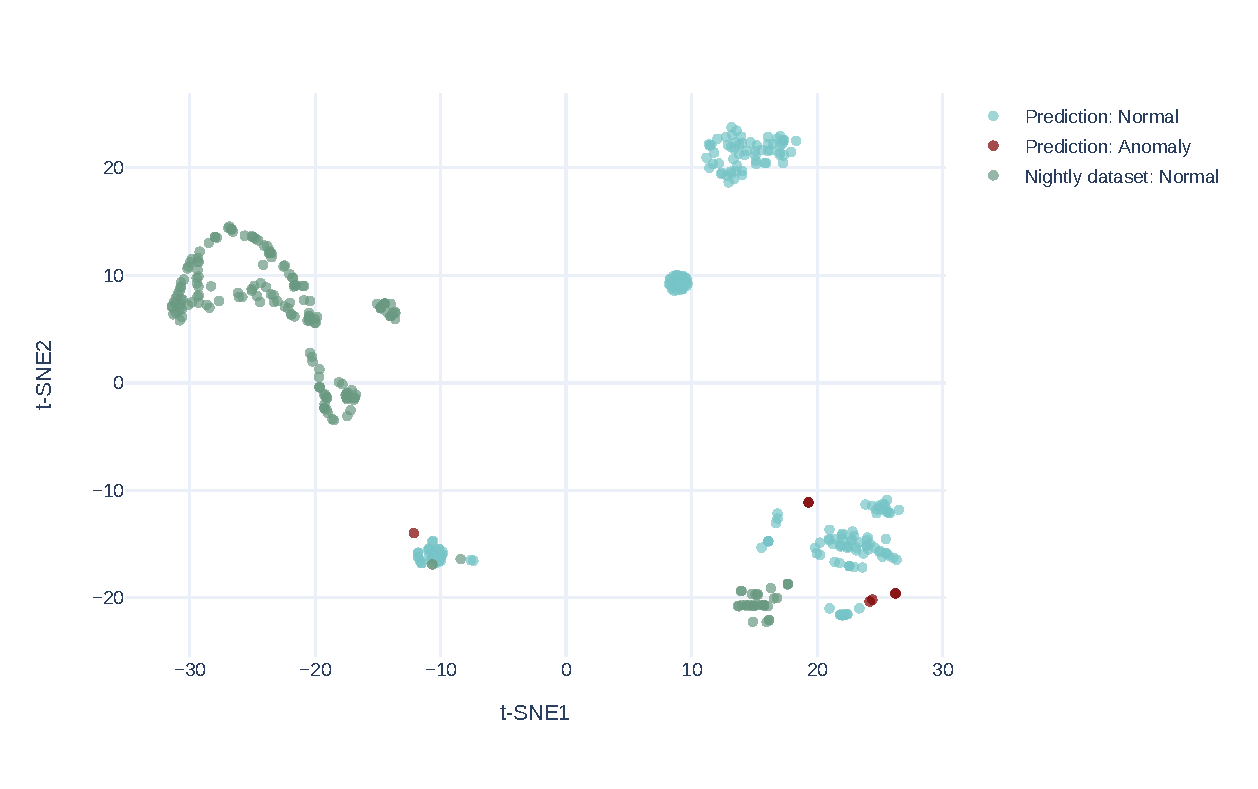
\includegraphics[width=0.9\textwidth]{img/tsne-predictions-unlabeled-isolation-forest.pdf} }}%
    \qquad
    \subfloat[\centering Invariants Mining]{{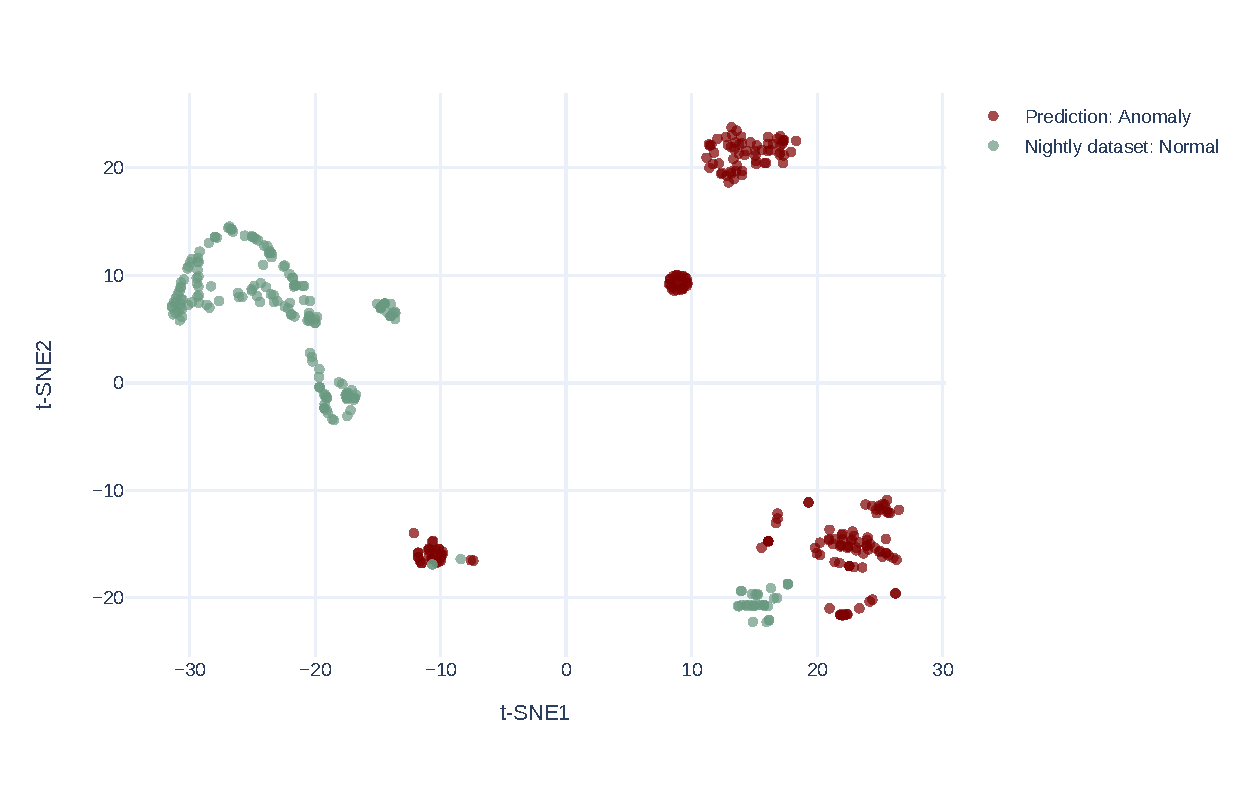
\includegraphics[width=0.9\textwidth]{img/tsne-predictions-unlabeled-invariants-mining.pdf} }}%
    \caption{Comparison of t-SNE applied on Isolation Forest (a) and Invariants Mining (b) predictions on the unlabeled Daily dataset. Green data points represent the normal datapoints as a point of reference, data points highlighted in blue and red represent predictions of normal or anomalous log sequence respectively.}%
    \label{fig:tsne-unlabeled-plots-appendix}%
\end{figure}

\begin{figure}%
    \centering
    \subfloat[\centering Isolation Forest]{{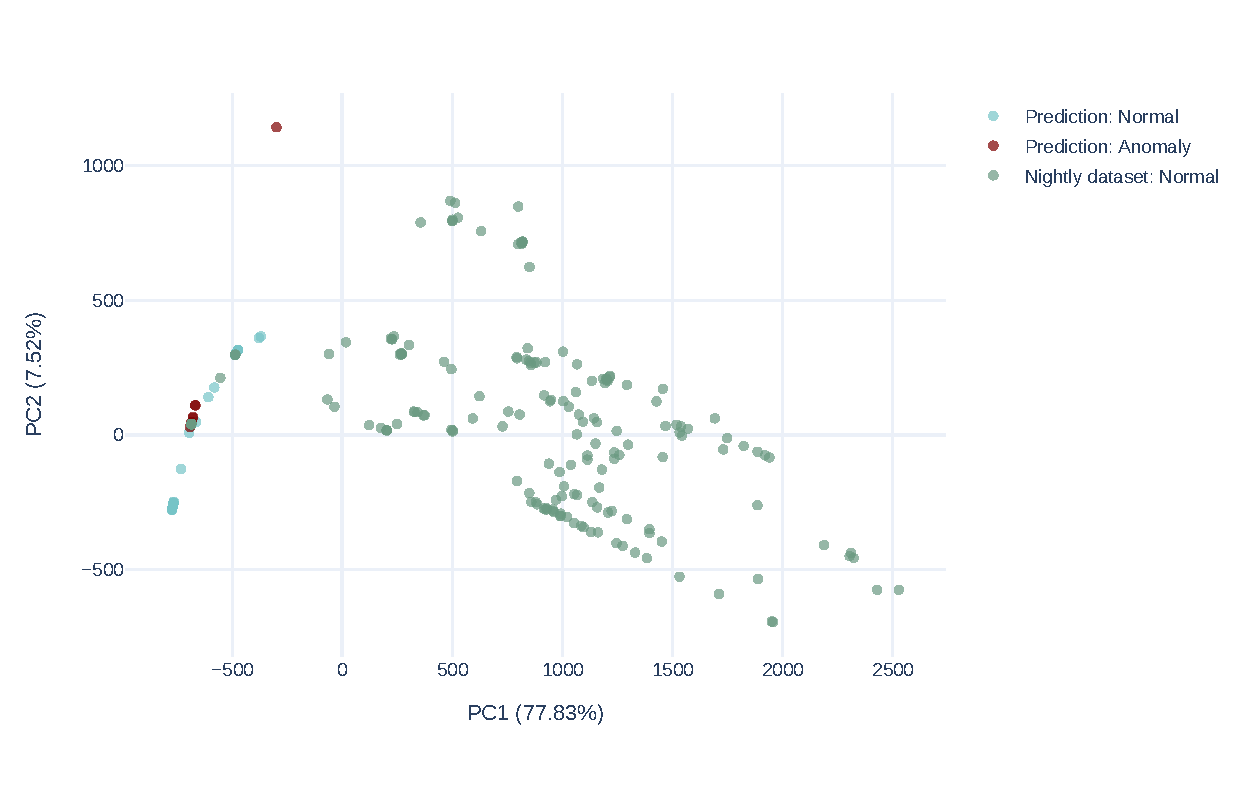
\includegraphics[width=7cm]{img/pca-predictions-unlabeled-isolation-forest.pdf} }}%
    \qquad
    \subfloat[\centering PCA]{{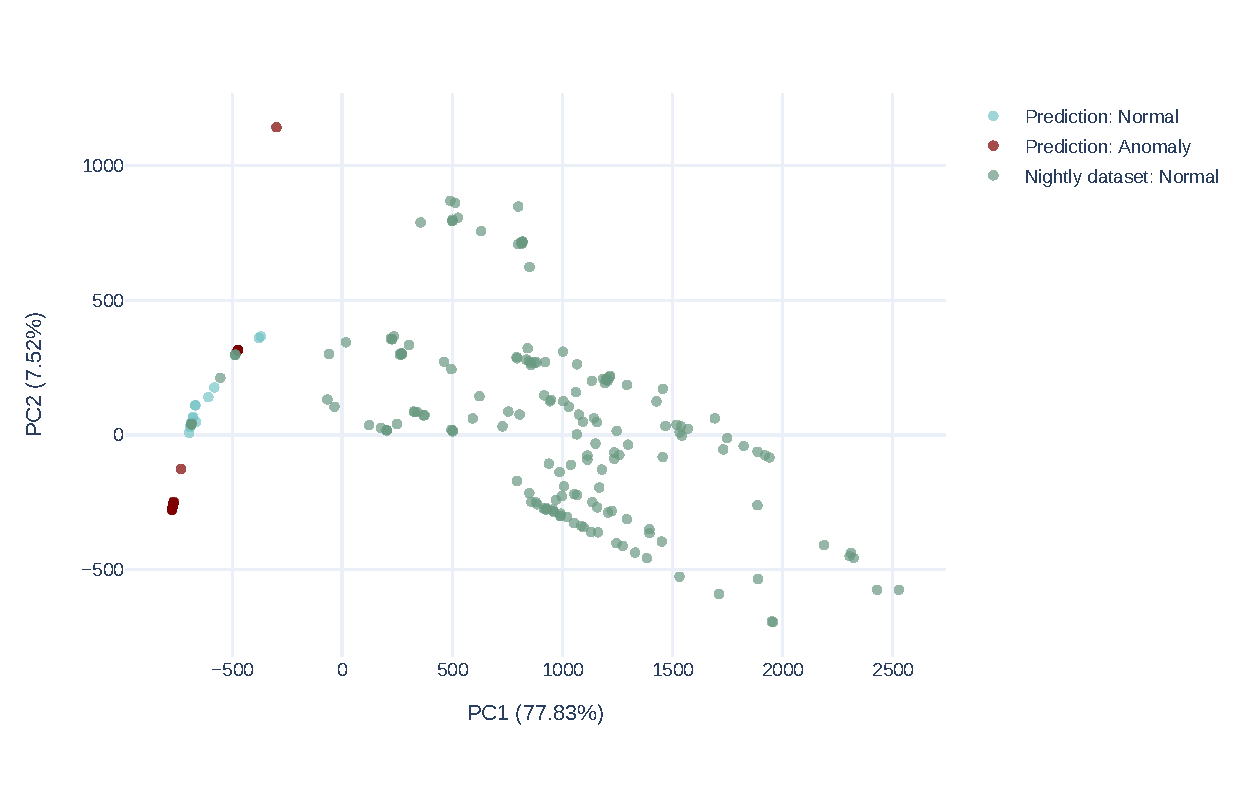
\includegraphics[width=7cm]{img/pca-predictions-unlabeled-pca.pdf} }}%
     \qquad
    \subfloat[\centering Invariants Mining]{{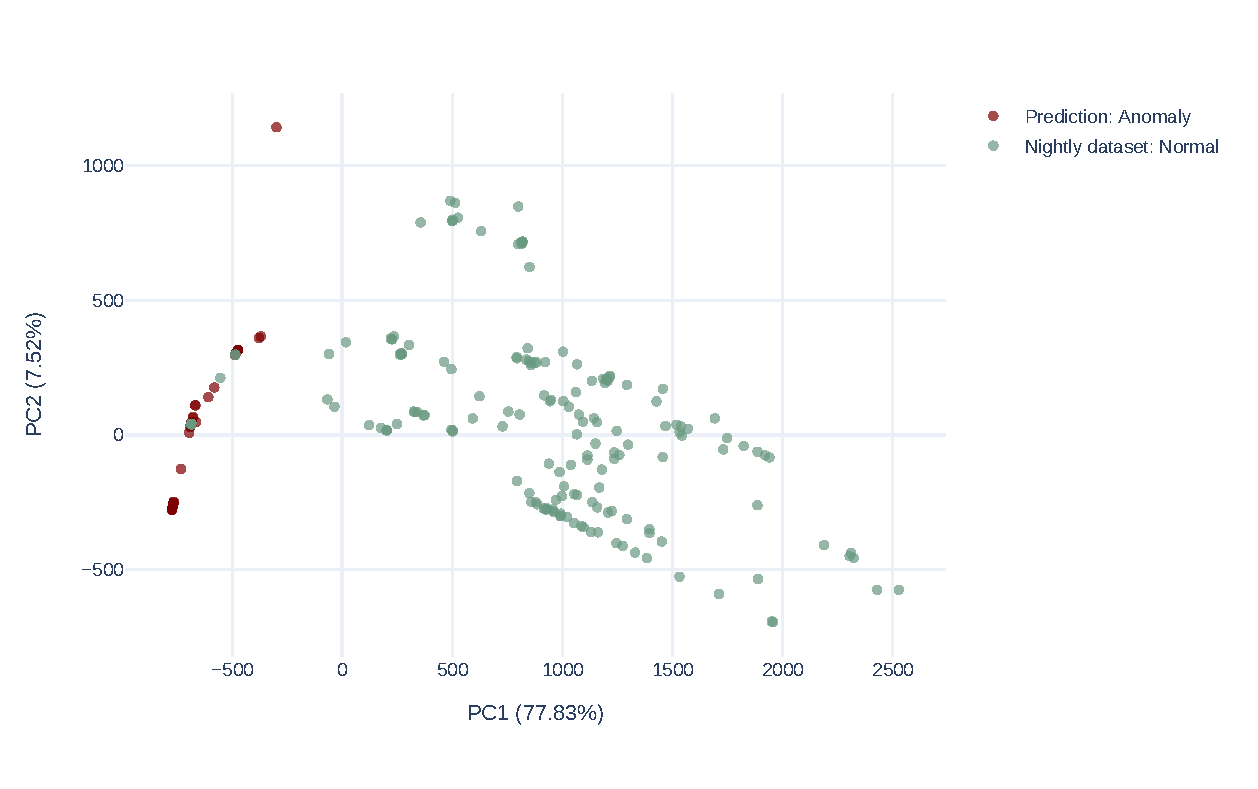
\includegraphics[width=7cm]{img/pca-predictions-unlabeled-invariants-mining.pdf} }}%
     \qquad
    \subfloat[\centering Log Clustering]{{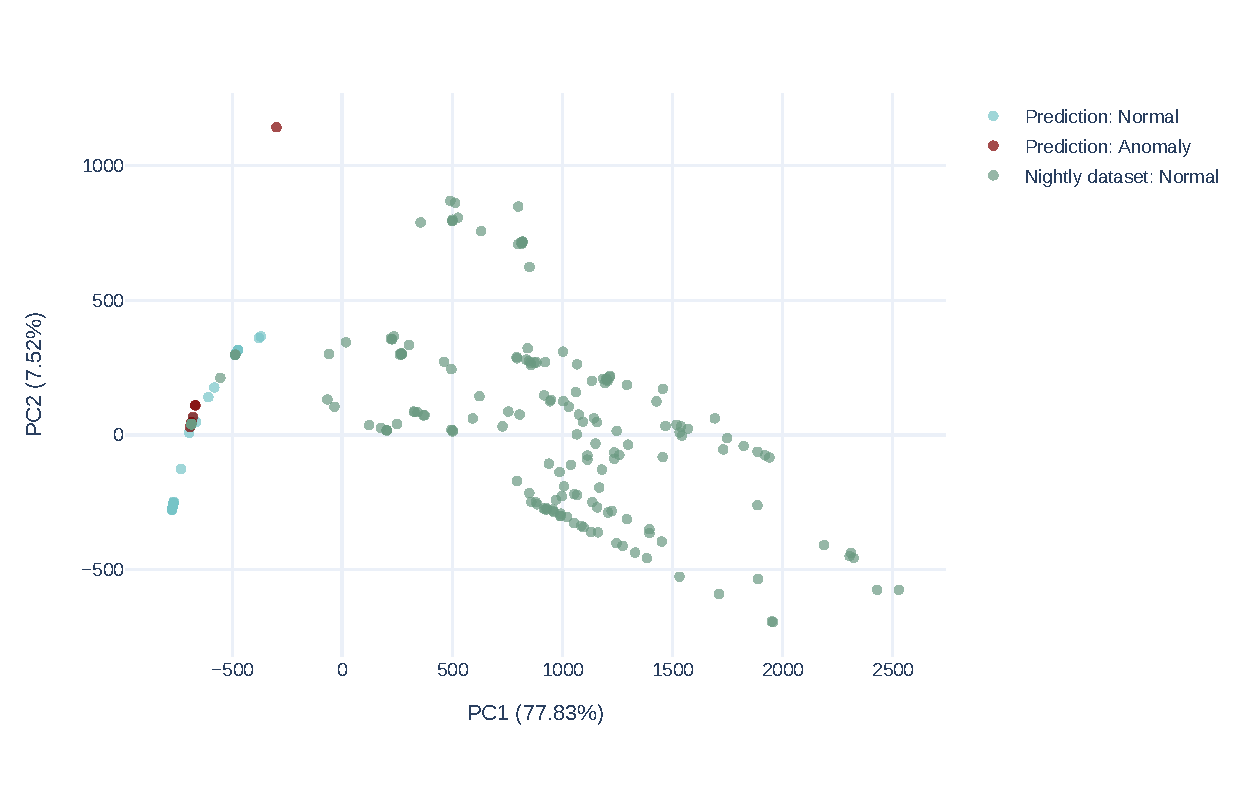
\includegraphics[width=7cm]{img/pca-predictions-unlabeled-clustering.pdf} }}%
    \caption{Comparison of PCA applied on Isolation Forest (a), PCA (b), Invariants Mining (c) and Log Clustering (d) predictions on the unlabeled Daily dataset. Green data points represent the normal datapoints as a point of reference, data points highlighted in blue and red represent predictions of normal or anomalous log sequence respectively.}%
    \label{fig:pca-unlabeled-plots-appendix}%
\end{figure}
\end{appendices}

\end{document}
%%  ==================================================================
%%  End document